\documentclass[twoside,notitlepage,11pt]{report}
%\usepackage{a4paper}
\usepackage{graphicx}
\usepackage{psfrag}
\usepackage{amsfonts}
\usepackage{amsmath}
\usepackage{amsbsy}
\usepackage{verbatimfile}
\usepackage{fancyhdr}
\usepackage{pstricks,pst-node}
% The next rawfonts package one is used in the ``datablad''.
\usepackage[only,egtrm]{rawfonts}
% Handle sorting in reference list
\usepackage{citesort}
% Create an index table
\usepackage{makeidx}

\newcommand{\smallverbatimfile}[1]{{\footnotesize\verbatimfile{#1}}}
\newcommand{\component}[5]{\begin{tabular}{|lp{0.7\textwidth}|}\hline {\bf Name:} & #1 \\ \hline {\bf Author:} & #2 \\ \hline {\bf Input parameters} & #3 \\ \hline {\bf Optional parameters} & #4 \\ \hline {\bf Notes} & #5 \\ \hline \end{tabular} \\ \noindent }

\def\reportnum{Ris{\o}--R--1538(EN)}

%\oddsidemargin 0cm
%\evensidemargin 0cm
\addtolength{\hoffset}{-1.4cm}
\topmargin 0cm
\textwidth 15cm
\textheight 22cm
\addtolength{\footskip}{1.6pt}
\addtolength{\headheight}{1.6pt}

\pagestyle{fancy}
\fancyhf{}
\fancyfoot[LE,RO]{\thepage}
\fancyfoot[LO,RE]{\reportnum}
\renewcommand{\headrulewidth}{0pt}
\renewcommand{\footrulewidth}{0pt}

\fancypagestyle{plain}{%
\fancyhf{}
\fancyfoot[LE,RO]{\thepage}
\fancyfoot[RE,LO]{\reportnum}
\renewcommand{\headrulewidth}{0pt}
\renewcommand{\footrulewidth}{0pt}}

\newcommand{\MCS}{{McStas}}
\newcommand{\version}{{1.10}}
\newcommand{\reldate}{{November, 2006}}
\newcommand{\Ombold}{\mbox{\boldmath $\Omega$}}

% enable index generation
\makeindex

%\title{Component manual\\ to the neutron ray-tracing package
% \MCS ,\\ version \version}
%\author{Kim Lefmann, Peter Kj\ae r Willendrup, and Kristian Nielsen, \\
% Materials Research Department, \\
% Ris\o\ National Laboratory, 4000 Roskilde, Denmark;\\
% Emmanuel Farhi and Klaus Lieutenant \\ ILL, Grenoble, France}
%\date{\reldate \\[2\baselineskip]
%\begin{center}
%  \includegraphics[width=4.5in]{figures/vanadium-surf-2.eps}
%\end{center}
%\includegraphics[width=0.45\myheight]{risoe-logo.eps}%
%}
\begin{document}

%\maketitle
% Emacs settings: -*-mode: latex; TeX-master: "manual.tex"; -*-

\begingroup                     % Make all definitions local.

%
% This was modified from risoe.sty, <2 Aug 95>
%
\catcode`\@=11
\def\@magscale#1{ scaled \magstep#1 }
\font\frtnbf = cmb10 \@magscale2
\font\twfvbf = cmbx10   \@magscale5 % extended bold
\def\maketitle{\par
 \begingroup
 \def\thefootnote{\fnsymbol{footnote}}
 \def\@makefnmark{\hbox to 0pt{$^{\@thefnmark}$\hss}}
 \if@twocolumn
 \twocolumn[\@maketitle]
 \else \newpage
 \global\@topnum\z@ \@maketitle \fi\thispagestyle{empty}\@thanks\newpage
 \endgroup
 \setcounter{footnote}{0}
 \let\maketitle\relax
 \let\@maketitle\relax
 \gdef\@thanks{}\gdef\@author{}\gdef\@title{}\let\thanks\relax}
\def\@maketitle{\newpage \baselineskip 30dd \mbox{}
 \marginpar{{\frtnbf \hfill \llap{\mbox{\reportnum \reportlan\qquad\qquad}}}}
 \par\noindent\mbox{\includegraphics[width=0.27\textwidth]{figures/risoe-logo.eps}} \par
 \vskip 1.5cm
 {\twfvbf \noindent \@title \par} \vskip 20dd \baselineskip 16dd
 {\frtnbf\noindent\@author \par} \par \vfill \baselineskip 12dd
 \frtnbf\noindent Ris{\o} National Laboratory, Roskilde, Denmark \par
 \vskip 4dd \noindent\ifcase\month\or
 January\or February\or March\or April\or May\or June\or
 July\or August\or September\or October\or November\or December\fi
 \space\number\year }

\let\reportlan=\relax
\def\month{5}                   % Released in May 2005
% Need to match front page line breaking.
\title{Component~Manual~for~\rlap{the}\\ % Avoid overfull message.
 Neutron~Ray-Tracing~Package\\
 \MCS,\\ Version \version\ }
\author{Peter Kj\ae r Willendrup, Kim Lefmann, Emmanuel Farhi, and Klaus Lieutenant}
\maketitle
\endgroup

%\begin{center}
%  \includegraphics[width=4.5in]{figures/sqw.eps}
%\end{center}
%
% NOTE: Find a way to include this nice graphics on front page
% Currently this does not work?!?

\thispagestyle{empty}
% Emacs settings: -*-mode: latex; TeX-master: "manual.tex"; -*-

\begin{abstract}
\input{abstract_comp}
\end{abstract}

\vskip\baselineskip\noindent
This report documents the components for McStas version \version,
released \reldate .
\vskip\baselineskip\noindent
The authors are:
\begin{quote}
\label{p:authors}
\vskip\baselineskip\noindent
Kim Lefmann \\
Materials Research Department, Ris{\o} National Laboratory, DTU, Roskilde, Denmark \\
email: \verb+kim.lefmann@risoe.dk+
\vskip\baselineskip\noindent
Peter Kj\ae r Willendrup \\
Materials Research Department, Ris{\o} National Laboratory, DTU, Roskilde, Denmark \\
email: \verb+peter.willendrup@risoe.dk+
\vskip\baselineskip\noindent
Kristian Nielsen \\
email: \verb+kristian.nielsen@mail.tele.dk+
\vskip\baselineskip\noindent
Emmanuel Farhi \\
Institut Laue-Langevin, Grenoble, France \\
email: \verb+farhi@ill.fr+
\vskip\baselineskip\noindent
Klaus Lieutenant \\
Institutt for Energiteknikk, Kjeller, Norway\\
email: \verb+Klaus.Lieutenant@ife.no+
\end{quote}
%Front page illustration:\\[\baselineskip]
%Simulated scattering from a vanadium sample
%taking into account the secondary extinction. See
%section~\ref{s:vanadium-result}.
\vfill
\noindent ISBN 978--87--550--3619--2
\par\noindent ISSN 0106--2840
\par\noindent\hbox{}\hfill
    Pitney Bowes Management Services Denmark A/S $\cdot$ Ris{\o} National Laboratory $\cdot$ \number\year
%    Information Service Department $\cdot$ Ris{\o} $\cdot$ \number\year
\par
\thispagestyle{empty}\clearpage


\tableofcontents
%\pagebreak
%\listoffigures
%\pagebreak
%\listoftables

% Emacs settings: -*-mode: latex; TeX-master: "manual.tex"; -*-

\addcontentsline{toc}{chapter}{\protect\numberline{}{Preface and acknowledgements}}
\chapter*{Preface and acknowledgements}
This document contains information on the neutron scattering components 
which are the building blocks for describing instruments 
in the Monte Carlo neutron
ray-tracing program \MCS\ version \version . This is an update to the initial
release in October 1998 of version 1.0 as presented in Ref.~\cite{nn_10_20}. 
The reader of this
document is not supposed to have specific knowledge of neutron scattering,
but some basic understanding of the underlying physics is helpful in
understanding the theoretical background for the component functionality. 
For details about simulation techniques, we refer to 
the McStas system manual \cite{mcstasmanual}.
We assume familiarity with the use of 
the C programming language.

We especially like to thank Kristian Nielsen for laying a solid foundation
for the \MCS\ system, which the authors of this manual are using daily.
It is also a pleasure to thank Prof.~Kurt N.~Clausen for his continuous
support to \MCS\ and for having initiated the project.
%Both he and our other collaborators, Henrik M.\ R\o nnow and Mark
%Hagen have made major contributions to the project.  Also the
%contributions from our test users, the students Asger Abrahamsen, Niels
%Bech Christensen, and Erik Lauridsen, are gratefully acknowledged; they
%gave us an excellent opportunity to pinpoint a vast amount of serious
%errors in the test version.  Useful comments to this document itself
%have been given by Bella Lake and Alan Tennant.  
We have also benefited
from discussions with many other people in the neutron scattering
community, too numerous to mention here.

%Philipp Bernhardt contributed the two chopper components in
%sections~\ref{s:chopper} and~\ref{s:first_chopper}. Emmanuel Farhi
%contributed the components in sections~\ref{s:sourceoptimizer},
%\ref{s:monitornd}, and~\ref{s:monitoroptimizer}. 
The users who contributed components to this manual are acknowledged
as authors of the individual components. We encourage other
users to contribute components with manual entries for inclusion in
future versions of \MCS.

In case of any errors, questions, suggestions, 
%or other need for support should arise,
do not hesitate to 
contact the authors at \verb+mcstas@risoe.dk+
or consult the \MCS\ WWW home page~\cite{mcstas_webpage}.

Important developments on the component side in \MCS\ version \version\ 
as compared to version 1.4 (the last version of the component manual) include

\begin{itemize}
\item I do not know what to say...
\end{itemize} 

The \MCS\ project has been supported by the European Union, initially
through the XENNI program and the RTD ``Cool Neutrons'' program.
Over the last 3 years, \MCS\ was supported strongly through the
``SCANS'' program.







% Emacs settings: -*-mode: latex; TeX-master: "manual.tex"; -*-

\chapter{About the component library}
\label{c:components}
The component library is
maintained by the \MCS\ system group. A number of basic components 
``belongs'' the \MCS\ system, and are supported and tested by the \MCS\
team.

Other components are contributed
by specific authors, who are listed at each component
they contribute.
\MCS\ users are encouraged to send their
contributions to us for inclusion in future releases.

In the description of the theory behind the component functionality 
we will use the usual symbols {\bf r} for the position 
$(x,y,z)$ of the particle (unit m), and {\bf v} for 
the particle velocity $(v_x, v_y, v_z)$ (unit m/s).
Another frequently used symbol is 
the wave vector ${\bf k} = m_{\rm N} {\bf v}/\hbar$ , where
$m_{\rm N}$ is the neutron mass. {\bf k} is usually given in
\AA$^{-1}$, while neutron energies are given in meV.
In general, vectors are denoted by boldface symbols.
Subscripts "i" and "f" denotes ``initial'' and ``final'', respectively,
and are used in connection with the neutron state before and after
an interaction with the component in question.
Note that all mentioning of component geometry refer to
the local coordinate system of the individual component.
The axis convention is so that the $z$ axis is along 
the neutron propagation axis, the $y$ axis is vertical up, 
and the $x$ completes the right-handed coordinate system.

Source code for all components may be found in the \verb+lib/mcstas/+
subdirectory of the McStas installation; 
the default is \verb+/usr/local/lib/mcstas/+ 
on Unix-like systems and \verb+C:\mcstas\lib+ on Windows systems, but it can be
changed using the \verb+MCSTAS+ environment variable. 
\index{Environment variable!MCSTAS}

As a complement to this Component Manual, we encourage users to use
the \verb+mcdoc+ front-end which enables to display both the 
catalog of the \MCS\ library, e.g using: \index{Tools!mcdoc}
\begin{quote}
  \verb|mcdoc --show|
\end{quote}
as well as the documentation of specific components, e.g with:
\begin{quote}
  \verb|mcdoc --text| {\it name} \\
  \verb|mcdoc --show| {\it file.comp}
\end{quote}
The first line will search for all components matching the {\it name}, 
and display their help section as text, 
whereas the second example will display the help corresponding to 
the {\it file.comp} component, using your 
BROWSER\index{Environment variable!BROWSER} setting, or as text if unset. 
The \verb+--help+ option will display the command help, as usual.

An overview of the component library is also given at the \MCS\ home page...

%% Emacs settings: -*-mode: latex; TeX-master: "manual.tex"; -*-

\section{Source components}
The main function of the source components is to determine a set of initial
parameters $({\bf r}, {\bf v})$, or equivalent (${\bf r}, v, \Ombold $),
for each neutron. This is done by Monte Carlo choices. 
In the current sources no polarization dependence is implemented, 
whence we let ${\bf s}=(0,0)$.

The sources to be presented in the following all make their Monte Carlo
choices on the basis of simple analytical expressions ({\em e.g.} the
energy distribution). 
More realistic sources would require that (at least) the Monte-Carlo choice
for the initial energy was made on basis of a measured,
tabulated energy spectrum.
This is planned to be implemented in a later version of \MCS .

\subsection{Source\_flat: A circular continuous source with a flat energy spectrum}
\label{sourceaim}
This component {\bf Source\_flat} is 
a simple continous source with a flat energy distribution.
The time-of-flight aspect is not relevant for this component,
so we put $t=0$ for all neutrons.

The initial neutron position is chosen randomly from within a
circle of radius $r_{\rm s}$ in the $z=0$ plane. 
This is a fair approximation
of a cylindrical cold source with the beam going out along
the cylinder axis, like the one at Ris\o .

The initial neutron velocity direction is focused within
a solid angle, defined by a rectangular target of width
$w$, height $h$, parallel to 
the $xy$ plane placed at $(0,0,z_{\rm f})$. 
A small angle approximation is used, assuming that 
$w,h \ll z_{\rm f}$.

The weight multiplier of the created neutron, $\pi_1$, is set to the
solid angle of the focusing opening divided by $4\pi$,
see discussion in \ref{s:focus}

The input parameters of {\bf Source\_flat} are the source radius, $r_{\rm s}$,
the distance to the target, $z_{\rm f}$, 
the dimensions of the target, $w$ and $h$, and
the centre and spread of the energy distribution, $E_0$ and $\Delta E$.


\subsection{Source\_flat\_lambda: A continous source with flat
  wavelength spectrum}

The component {\bf Source\_flat\_lambda} is similar to the Source\_flat
component, except that the spectrum is flat in wavelength, rather
than in energy.

The input parameters for Source\_flat\_lambda are \textit{radius} to set
the source radius in meters; \textit{dist}, \textit{xw}, and \textit{yh}
to set the focusing as for Source\_flat; and \textit{lambda\_0} and
\textit{d\_lambda} to set the range of wavelength emitted (the range
will be from $\textit{lambda\_0} - \textit{d\_lambda}$ to
$\textit{lambda\_0} + \textit{d\_lambda}$).


\subsection{Source\_flux\_lambda: A continuous source with absolute
  flux}
\label{Source_flux_lambda}

The component {\bf Source\_flux\_lambda} is a variation on the
Source\_flat\_lambda component. The only difference is the possibility
to specify the absolute flux of the source. The specified flux is used
to adjust the initial neutron weight so that the intensity in the
detectors is directly comparable to a measurement of one second on a
real source with the same flux. This also makes the simulated detector
intensities independent of the number of neutron histories simulated,
easing the comparison between different simulation runs (though of
course more neutron histories will give better statistics).

The flux~$\Phi$ is the number of neutrons emitted per second from a
one~cm$^2$ area on the source surface, with direction within a a one
steradian solid angle, and with wavelength within a one {\AA}ngstr{\o}m
interval. The total number of neutrons emitted towards a given diaframe
in one second is therefore
$$ N_{\rm total} = \Phi A \Omega \Delta\lambda $$
where $A$ is the source area, $\Omega$ is the solid angle of the
diaframe as seen from the source surface, and $\Delta\lambda$ is the
width of the wavelength interval in which neutrons are emitted (assuming
a uniform wavelength spectrum). If $N_{\rm sim}$ denotes the number of
neutron histories to simulate, the initial neutron weight $p_0$ must be set to
$$ p_0 = \frac{N_{\rm total}}{N_{\rm sim}} = 
    \frac{\Phi}{N_{\rm sim}} A \Omega \Delta\lambda $$

The input parameters for Source\_flux\_lambda are \textit{radius} to set
the source radius in meters; \textit{dist}, \textit{xw}, and \textit{yh}
to set the focusing as for Source\_flat; \textit{lambda\_0} and
\textit{d\_lambda} to set the range of wavelength emitted (the range
will be from $\textit{lambda\_0} - \textit{d\_lambda}$ to
$\textit{lambda\_0} + \textit{d\_lambda}$); and \textit{flux} to set the
source flux in units of ${\rm cm}^{-2} {\rm st}^{-1} \textit{\AA}$.


\subsection{Source\_div: A divergent source}

{\bf Source\_div} is a rectangular source which emits a
beam of a certain divergence around the main exit direction
(the direction of the $z$ axis).
The beam intensity and divergence are uniform over
the whole of the source, and the energy distribution
of the beam is uniform.

This component may be used as a simple model of the
beam profile at the end of a guide or at the sample
position.

The input parameters for Source\_div are the source dimensions
$w$ and $h$ (in m), the divergencies $\delta_h$ and $\delta_v$ (FWHM in degrees), 
and the mean energy $E_0$ and the energy spread $dE$ (both in meV).
The neutron energy range is $(E_0-dE; E_0+dE)$. 


\subsection{Moderator: A time-of-flight source}
The simple time-of-flight source component {\bf Moderator} resembles
the source component {\bf Source\_flat} described in \ref{sourceaim}.
Like {\bf Source\_flat}, {\bf Moderator} is circular and focuses
on a rectangular target. Further, the initial velocity is chosen
with a linear distribution within an interval, defined by the
minimum and maximum energies, $E_0$ and $E_1$,
respectively.

The initial time of the neutron is determined on basis of a 
simple heuristical model for the time dependence of the 
neutron intensity from a time-of-flight source.
For all neutron energies, the flux decay is assumed to be exponential,
\begin{equation}
\Psi(E,t) = \exp(-t/\tau(E)) ,
\end{equation}
where the decay constant is given by
\begin{equation}
\tau(E) = \left\{ 
\begin{array}{cc}
 \tau_0                               & ; E<E_c \\
 \tau_0 / [ 1 + (E-E_c)^2/\gamma^2 ]  & ; E \geq E_c
\end{array}
\right.
\end{equation}

The input parameters for {\bf Moderator} are the source radius, $r_{\rm s}$,
the minimum and maximum energies, $E_0$ and $E_1$ (in meV),
the distance to the target, $z_{\rm f}$, the dimensions of the target,
$w$ and $h$, and the decay parameters 
$\tau_0$ (in $\mu$s), $E_c$, and $\gamma$ (both in meV).


% Emacs settings: -*-mode: latex; TeX-master: "manual.tex"; -*-

\section{Source\_adapt: A neutron source with adaptive importance sampling}
\label{s:Source_adapt}
\label{s:source-adapt}
\index{s:source-adapt}
\index{Optimization}

The {\bf Source\_adapt} component is a neutron source that uses adaptive
importance sampling to improve the efficiency of the simulations. It
works by changing on-the-fly the probability distributions from which
the initial neutron state is sampled so that samples in regions that
contribute much to the accuracy of the overall result are preferred over
samples that contribute little. The method can achieve improvements of a
factor of ten or sometimes several hundred in simulations where only a
small part of the initial phase space contains useful neutrons.
On the other side, a warning is in place here regarding potential wrong results using optimization techniques (see section \ref{s:optim} of the \MCS\ user manual). It is highly recommanded in any case to benchmark 'optimized' simulations against non-optimized ones, checking that obtained results are the same, but hopefully with a much improved statistics.

The physical characteristics of the source are similar to those of
Source\_flat (see section~\ref{sourceaim}). The source is a thin
rectangle in the $X$-$Y$ plane with a flat energy spectrum in a
user-specified range. The flux per area per steradian per
{\AA}ngstr{\o}m per second is specified by the user; the total weight of
neutrons emitted from the source will then be the same irrespectively of
the number of neutron histories simulated, corresponding to one second
of measurements.

The initial neutron weight is given by (see
section~\ref{Source_flux_lambda} for details)
$$ p_0 = \frac{N_{\rm total}}{N_{\rm sim}} =
    \frac{\Phi}{N_{\rm sim}} A \Omega \Delta\lambda $$
Here $\Delta\lambda$ is the total wavelength range of the source; since
the spectrum is flat in energy (but not in wavelength), the flux
will actually be different for different energies. A later version of
this component will probably adapt (in a backward-compatible way) a more
sensible way to specify the flux. For now, an energy or wavelength
monitor (see sections~\ref{s:e_monitor} and~\ref{s:L_monitor}) placed
just after the source will show the actual energy-dependent flux.


\subsection{The adaption algorithm}

The adaptive importance sampling works by subdividing the initial
neutron phase space into a number of equal-sized bins. The division is
done on the three dimensions of energy, horizontal position, and
horizontal divergence, using $N_{\rm eng}$, $N_{\rm pos}$, and $N_{\rm
  div}$ number of bins in each dimension, respectively. The total number
of bins is therefore
$$
N_{\rm bin} = N_{\rm eng} N_{\rm pos} N_{\rm div}
$$
Each bin $i$ is assigned a sampling weight $w_i$; the probability of
emitting a neutron within bin $i$ is
$$
P(i) = \frac{w_i}{\sum_{j=1}^{N_{\rm bin}} w_j}
$$
In order to avoid false learning, the sampling weight of a bin is
kept larger than $w_{\rm min}$, defined as
$$
w_{\rm min} = \frac{\beta}{N_{\rm bin}}\sum_{j=1}^{N_{\rm bin}}w_j,\qquad
    0 \leq \beta \leq 1
$$
This way a (small) fraction $\beta$ of the neutrons are sampled
uniformly from all bins, while the fraction $(1 - \beta)$ are sampled in an adaptive way.

Compared to a uniform sampling of the phase space (where the probability
of each bin is $1/N_{\rm bin}$), the neutron weight
must be adjusted by the amount
$$
\pi_i = \frac{1/N_{\rm bin}}{P(i)} =
    \frac{\sum_{j=1}^{N_{\rm bin}} w_j}{N_{\rm bin} w_i}
$$

In order to set the criteria for adaption, the Adapt\_check component is
used (see section~\ref{s:adapt_check}). The source attemps to sample
only from bins from which neutrons are not absorbed prior to the
position in the instrument at which the Adapt\_check component is
placed. Among those bins, the algorithm attemps to minimize the variance
of the neutron weights at the Adapt\_check position. Thus bins that
would give high weights at the Adapt\_check position are sampled more
often (lowering the weights), while those with low weights are sampled
less often.

Let $\pi = p_1/p_0$ denote the ratio between the neutron weight $p_1$ at
the Adapt\_check position and the initial weight $p_0$ just after the
source. For each bin, the component keeps track of the sum $\psi$ of
$\pi$'s as well as of the total number of neutrons $n_i$ from that
bin. The average weight at the Adapt\_source position of bin $i$ is thus
$\psi_i/n_i$.

We now distribute a total sampling weight of $\beta$ uniformly
among all the bins, and a total weight of $(1 - \beta)$ among bins in
proportion to their average weight $\psi_i/n_i$ at the Adapt\_source
position:
$$
w_i = \frac{\beta}{N_{\rm bin}} +
    (1-\beta) \frac{\psi_i/n_i}{\sum_{j=1}^{N_{\rm bins}} \psi_j/n_j}
$$
After each neutron event originating from bin $i$, the sampling weight $w_i$
is updated.

This basic idea can be improved with a small modification. The problem
is that until the source has had the time to learn the right sampling
weights, neutrons may be emitted with high neutron weights (but low
probability). These low probability neutrons may account for a large fraction of
the total intensity in detectors, causing large variances in the
result. To avoid this, the component emits early neutrons with a lower
weight, and later neutrons with a higher weight to compensate. This way
the neutrons that are emitted with the best adaption contribute the most
to the result.

The factor with which the neutron weights are adjusted is given by a
logistic curve
\begin{equation}
  F(j) = C\frac{y_0}{y_0 + (1 - y_0) e^{-r_0 j}}
\end{equation}
where $j$ is the index of the particular neutron history, $1 \leq j
\leq N_{\rm hist}$. The constants $y_0$, $r_0$, and $C$ are given by
\begin{eqnarray}
  y_0 &=& \frac{2}{N_{\rm bin}} \\
  r_0 &=& \frac{1}{\alpha}\frac{1}{N_{\rm hist}}
     \log\left(\frac{1 - y_0}{y_0}\right) \\
  C &=& 1 + \log\left(y_0 + \frac{1 - y_0}{N_{\rm hist}}
     e^{-r_0 N_{\rm hist}}\right)
\end{eqnarray}
The number $\alpha$ is given by the user and specifies (as a fraction
between zero and one) the point at which the adaption is considered
good. The initial fraction $\alpha$ of neutron histories are emitted
with low weight; the rest are emitted with high weight:
$$ p_0(j) =
    \frac{\Phi}{N_{\rm sim}} A \Omega \Delta\lambda
    \frac{\sum_{j=1}^{N_{\rm bin}} w_j}{N_{\rm bin} w_i}
    F(j)
$$
The choice of the constants $y_0$, $r_0$, and $C$ ensure that
$$
\int_{t=0}^{N_{\rm hist}} F(j) = 1
$$
so that the total intensity over the whole simulation will be correct

Similarly, the adjustment of sampling weights is modified so that the
actual formula used is
$$
w_i(j) = \frac{\beta}{N_{\rm bin}} +
    (1-\beta) \frac{y_0}{y_0 + (1 - y_0) e^{-r_0 j}}
     \frac{\psi_i/n_i}{\sum_{j=1}^{N_{\rm bins}} \psi_j/n_j}
$$

\subsection{The implementation}

\component{Source\_adapt}{K. Nielsen}{$x_{min}$, $x_{max}$, $y_{min}$, $y_{max}$, $E0$, $dE$, dist, $xw$, $yh$, $Phi$}{$\alpha$, $\beta$ (plenty, default values are ok)}{not fully validated}

The heart of the algorithm is a discrete distribution $p$. The
distribution has $N$ \emph{bins}, $1\ldots N$. Each bin has a value
$v_i$; the probability of bin $i$ is then $v_i/(\sum_{j=1}^N v_j)$.

Two basic operations are possible on the distribution. An \emph{update}
adds a number $a$ to a bin, setting $v_i^{\rm new} = v_i^{\rm old} +
a$. A \emph{search} finds, for given input $b$, the minimum $i$ such
that
$$ b \leq \sum_{j=1}^{i} v_j. $$
The search operation is used to sample from the distribution p. If $r$
is a uniformly distributed random number on the interval
$[0;\sum_{j=1}^N v_j]$ then $i = {\rm search}(r)$ is a random number
distributed according to $p$. This is seen from the inequality
$$ \sum_{j=1}^{i-1} v_j < r \leq \sum_{j=1}^{i} v_j, $$
from which $r \in [\sum_{j=1}^{i-1} v_j; v_i + \sum_{j=1}^{i-1} v_j]$
which is an interval of length $v_i$. Hence the probability of $i$ is
$v_i/(\sum_{j=1}^N v_j)$.
The update operation is used to
adapt the distribution to the problem at hand during a simulation. Both
the update and the add operation can be performed very efficiently; how
this is achieved will be described elsewhere.

The input parameters for Source\_adapt are
\textit{xmin}, \textit{xmax}, \textit{ymin}, and
\textit{ymax} in meters to set the source dimensions;
\textit{dist}, \textit{xw}, and \textit{yh}
to set the focusing as for Source\_flat (section~\ref{sourceaim}); \textit{E0} and
\textit{dE} to set the range of energies emitted, in meV (the range
will be from $\textit{E0} - \textit{dE}$ to
$\textit{E0} + \textit{dE}$); flux to set the source flux $\Phi$ in ${\rm
  cm}^{-2} {\rm st}^{-1} \textit{\AA} {\rm s}^{-1}$;
$N_{\rm eng}$, $N_{\rm pos}$, and $N_{\rm
  div}$ to set the number of bins in each dimensions; \textit{alpha} and
\textit{beta} to set the parameters $\alpha$ and $\beta$ as described
above; and \textit{filename} to give the name of a file in which to
output the final sampling destribution.

A good general-purpose value for $\alpha$ and $\beta$ is $\alpha = \beta
= 0.25$. The number of bins to choose will depend on the
application. More bins will allow better adaption of the sampling, but
will require more neutron histories to be simulated before a good
adaption is obtained. The output of the sampling distribution is only
meant for debugging, and the units on the axis are not necessarily
meaningful. Setting the filename to \verb+NULL+ disables the output of
the sampling distribution.

As an alternative, you may use the Source\_Optimizer component (see section \ref{source-optimizer}).


\input{Source_Optimizer}

%% Emacs settings: -*-mode: latex; TeX-master: "manual.tex"; -*-

\section{Simple optical components:
Arms, slits, collimators, filters}
Below we list a number of simple optical components 
which require only a minimum of explanation.

\subsection{Arm: The generic component}
\label{explain:arm}
The component {\bf Arm} is empty; is resembles an optical bench
and has no effect on the neutron.
The function of this component is only to set up a local frame of
reference within the instrument definition. Other components of the
same arm/optical bench may then be
positioned relative to the arm component
using the \MCS\ meta-language.
The use of arm components in the instrument definitions
is not required but is recommended for clarity.

{\bf Arm} has no input parameters.
For more about the use of this component, see the 
sample instrument definitions listed in Appendix \ref{instcode}.


\subsection{Slit: The rectangular slit}
\label{slit}
The component {\bf Slit} is a very simple construction.
It sets up a rectangular opening at $z=0$, and propagates the neutrons 
onto the plane of this rectangle by the kernel call PROP\_Z0.

Neutrons within the slit opening are unaffected, 
while all other neutrons
(no matter how far from the opening their paths intersect the plane)
are discarded by the kernel call ABSORB.
By this simplification, some neutrons contributing to the background
in a real experiment will be neglected. 
These are the ones that scatter off the inner side
of the slit, penetrates the slit material, 
or that clear one of the outer edges of the slit.

The input parameters of {\bf Slit} are the four coordinates,
$(x_{\rm min}, x_{\rm max}, y_{\rm min}, y_{\rm max})$
defining the opening of the rectangle.

\subsection{Circular\_slit: The circular slit}
The component {\bf Circular\_slit} defines a circle in the $z=0$ plane,
centered in the origin. In analogy with {\bf Slit},
neutrons are propagated to this plane, and those which intersect
the plane outside the circle are ABSORB'ed.

The only input parameter of {\bf Circular\_slit} is
the radius, $r$, of the circle.

\subsection{Beamstop\_rectangular: The rectangular beam stop}
\label{s:Beamstop_rectangular}
The component {\bf Beamstop\_rectangular} models a thin, infinitely
absorbing rectangle in the $X$-$Y$ plane, centered on the origin. The
input parameters are \textit{xmin}, \textit{xmax}, \textit{ymin}, and
\textit{ymax} defining the edges of the slit in meters.


\subsection{Beamstop\_circular: The circular beam stop}
\label{s:Beamstop_circular}
The component {\bf Beamstop\_circular} models a thin, infinitely
absorbing circular disk in the $X$-$Y$ plane, centered on the origin. It
takes a single input parameter \textit{radius} to define the circle
radius in meters.


\subsection{Soller: The simple Soller blade collimator}
The component {\bf Soller} defines two rectangular openings
like the one in {\bf Slit}. Neutrons not clearing both these
openings are ABSORB'ed, see the discussion in \ref{slit}.
The collimating effect is taken care of by employing an ideal
triangular transmission through the collimator, as explained below.
For a more detailed Soller collimator simulation the Channeled\_guide
component can be employed, see section~\ref{s:channeled_guide}.

Let the collimation angle be $\delta = \tan^{-1}(d/L)$,
where $L$ is the length of the collimator
and $d$ is the distance between the blades,
and let $\phi$ be the divergence angle between the 
neutron path and a vertical plane along the collimator axis, 
see Fig.~\ref{f:collimator}. Neutrons with a large 
divergence angle $|\phi| \geq \delta$ will always
hit at least one collimator blade and will thus be absorbed.
For smaller divergence angles, $|\phi| < \delta$, the fate of the
neutron depends on its exact entry point.
Assuming that a typical collimator has many blades, the
absolute position of each blade perpendicular to the collimator axis
is somewhat uncertain (and also unimportant).
A simple statistical consideration now shows that the transmission
probability is $T = 1-\tan|\phi|/\tan\delta$.

\begin{figure}
  \begin{center}
    \psfrag{xmin}[c][c]{$x_{\rm min}$}
    \psfrag{xmax}[c][c]{$x_{\rm max}$}
    \psfrag{ymin}[c][c]{$y_{\rm min}$}
    \psfrag{ymax}[c][c]{$y_{\rm max}$}
    \psfrag{delta}[c][c]{$\delta$}
    \includegraphics[width=0.9\textwidth]{figures/collimator.eps}
  \end{center}
\caption{The geometry of a simple Soller blade collimators:
The real Soller collimator, seen from the top (left), 
and a sketch of the component {\bf Soller} (right).
The symbols are defined in the text.}
\label{f:collimator}
\end{figure}

We simulate the collimator by transmitting all neutrons with
$|\phi| < \delta$, but adjusting their weight with the amount
\begin{equation}
\pi_i = T = 1-\tan|\phi|/ \tan\delta ,
\end{equation}
while all others are discarded by the kernel call ABSORB.

The input parameters for {\bf Soller} are the coordinates
$(x_{\rm min}, x_{\rm max}, y_{\rm min}, y_{\rm max})$,
defining the identical entry and exit apertures, 
the length, $l$, between the slits, 
and the collimator divergence $\delta$.
If $\delta=0$, the collimating effect is disabled,
so that $\pi_i = 1$ whenever the neutron clears the two apertures.

\subsection{Filter: A transmission filter}
A neutron transmission filter act in much of the same way as two
identical slits, one after the other.
The only difference is that the transmission of the filter
varies with the neutron energy.

In the simple component {\bf Filter},
we have not tried to simulate the details of the transmission
process (which includes absorption, incoherent scattering,
and Bragg scattering in a polycrystalline sample, {\em e.g.} Be).
Instead, the transmission is parametrised to be
$\pi_i=T_0$ when $E \leq E_{\rm min}$, $\pi_i=T_1$ when $E \geq E_{\rm max}$,
and linearly interpolated between the two values
in the intermediate interval.
\begin{equation}
\pi_i = \left\{ \begin{array}{lc}
 T_0  & E \leq E_{\rm min} \\
 T_1 + (T_0-T_1) \frac{E_{\rm max}-E}{E_{\rm max}-E_{\rm min}}
 & E_{\rm min} < E < E_{\rm max} \\
 T_1  & E_\geq E_{\rm max} \\
\end{array} \right.
\end{equation}
If $T_1=0$, the neutrons with $E>E_{\rm max}$ are ABSORB'ed.

The input parameters are the four slit coordinates, 
$(x_{\rm min}, x_{\rm max}, y_{\rm min}, y_{\rm max})$,
the distance, $l$, between the slits, and the transmission parameters 
$T_0$, $T_1$, $E_{\rm min}$, and $E_{\rm max}$. 
The energies are given in meV.

%% Emacs settings: -*-mode: latex; TeX-master: "manual.tex"; -*-

\section{Advanced optical components: mirrors and guides}

This section describes advanced neutron optical
components such as supermirrors and guides.
The first subsection, however, contains 
only a description of the reflectivity of a supermirror.

\subsection{Mirror reflectivity}
\label{s:mirrorreflect}
To compute the reflectivity of the supermirrors, we use an empirical
formula derived from experimental data (see figure~\ref{f:reflectivity}). 
The reflectivity is given by the following formula
\begin{equation}
  R = \left\{
    \begin{array}{ll}
      R_0 & \textrm{if $Q \leq Q_{\rm c}$} \\
      \frac{1}{2}R_0(1 - \tanh[(Q - m Q_{\rm c})/W])(1-\alpha(Q-Q_{\rm c}))
         & \textrm{if $Q > Q_{\rm c}$}
    \end{array}
  \right.
\end{equation}

\begin{figure}
  \begin{center}
    \includegraphics[width=0.6\textwidth]{figures/supermirror.eps}
  \end{center}
\caption{A typical reflectivity curve for a supermirror,
Eq.~(\protect\ref{e:reflectivity}).}
\label{f:reflectivity}
\end{figure}
Here $Q$ is the length of the scattering vector (in \AA$^{-1}$)
defined by
\begin{equation} \label{e:reflectivity}
Q = |{\bf k}_{\bf i} - {\bf k}_{\bf f}| 
  = \frac{m_{\rm n}}{\hbar} |{\bf v}_{\bf i} - {\bf v}_{\bf f}|, 
\end{equation}
$m_{\rm n}$ being the neutron mass. 
The value $m$ is a parameter determined by the mirror materials,
the bilayer sequence, and the number of bilayers.
As can be seen, $R=R_0$ for $Q < Q_{\rm c}$, which is the
critical scattering wave vector for a single layer of the mirror
material. At higher values of $Q$, the reflectivity starts falling
linearly with a slope $\alpha$ until a cut-off at $Q = m Q_{\rm c}$. 
The width of the cut-off is denoted $W$. For the curve in
figure~\ref{f:reflectivity}, the values are
$$ m=4 \qquad R_0=1 \qquad Q_{\rm c} = 0.02\mbox{ \AA}^{-1} \qquad
   \alpha = 6.49\mbox{ \AA} \qquad W=1/300\mbox{ \AA}^{-1} $$
As a special case, if $m=0$ then the reflectivity is zero for all $Q$,
   \textit{ie.} the surface is completely absorbing.

In the components, the neutron weight is adjusted with the amount $\pi_i = R$. 
To avoid spending large amounts of computation time on very low-weight
neutrons, neutrons for which the reflectivity is lower than about
$10^{-10}$ are ABSORB'ed.

\subsection{Mirror: The single mirror}

The component {\bf Mirror} 
models a single rectangular neutron mirror plate. It can
be used to \textit{e.g.}~assemble a complete neutron guide by putting multiple
mirror components at appropriate locations and orientations in the
instrument definition, much like a real guide is build from individual
mirrors.

The mirror is assumed to lie in the first quadrant of the
$x$-$y$ plane, with one corner at $(0,0,0)$. 
If the neutron trajectory intersects the mirror plate, it is
reflected, otherwise it is left untouched. Since the mirror lies in the
$x$-$y$ plane, an incoming neutron with velocity 
${\bf v}_{\rm i} = (v_x,v_y,v_z)$
is reflected with velocity ${\bf v}_{\rm f} = (v_x,v_y,-v_z)$. 
The computation of the reflectivity is handled as detailed in
section~\ref{s:mirrorreflect}.

The input parameters of this component are
the rectangular mirror dimensions $(l, h)$
and the values of $R_0, m, Q_c, W$, and $\alpha$ for the mirror.


\subsection{Guide: The guide section}

The component {\bf Guide} 
models a guide tube consisting of four flat mirrors. The
guide is centered on the $z$ axis with rectangular entrance and exit
openings parallel to the $x$-$y$ plane. The entrance has the dimensions
$(w_1,h_1)$ and placed at $z=0$. The exit is of dimensions $(w_2,h_2)$
and is placed at $z=l$ where $l$ is the guide length. See
figure~\ref{f:guide}. Neutrons not clearing the guide entrance are
ABSORB'ed. For a more general guide simulation, see the Channeled\_guide
component in section~\ref{s:channeled_guide}.

\begin{figure}
  \begin{center}
    \includegraphics[width=0.9\textwidth]{figures/guide1.eps}
  \end{center}
\caption{The geometry used for the guide component.}
\label{f:guide}
\end{figure}

For computations on the guide geometry, we define the planes of the four
guide sides by giving their normal vectors (pointing into the guide)
and a point lying in the plane:
$$
\begin{array}{rclcrcl}
{\bf n}^v_1 &=& (l, 0, {(w_2 - w_1) / 2})
     & & {\bf O}^v_1 &=& (- w_1 / 2, 0, 0) \\
{\bf n}^v_2 &=& (-l, 0, {(w_2 - w_1) / 2})
     & & {\bf O}^v_2 &=& (w_1 / 2, 0, 0) \\
{\bf n}^h_1 &=& (0, l, {(h_2 - h_1) / 2})
     & & {\bf O}^h_1 &=& (0, - h_1 / 2, 0) \\
{\bf n}^h_2 &=& (0, -l, {(h_2 - h_1) / 2})
     & & {\bf O}^h_2 &=& (0, h_1 / 2, 0) \\
\end{array}
$$
In the following, we refer to an arbitrary guide side by its origin
{\bf O} and normal {\bf n}.

With these definitions, the time of intersection of the neutron with a
guide side can be computed by considering the projection onto the
normal:
\begin{equation} 
t_1 = {({\bf O} - {\bf r}_0) \cdot {\bf n} \over {\bf v} \cdot {\bf n}} 
\end{equation}
For a neutron that leaves the guide through the guide exit we have
\begin{equation}
t_2 = {l - z_0 \over v_z} 
\end{equation}
To compute the interaction of the neutron
with the guide, the neutron is initially propagated to the $z = 0$ plane of the
guide entrance. If it misses the entrance, it is ABSORB'ed. Otherwise,
we repeatedly compute the time of intersection with the
four mirror sides and the guide exit. The smallest positive $t$ thus
found gives the time of the next intersection with the guide (or in the
case of the guide exit, the time when the neutron leaves the guide). The
neutron is propagated to this point, the reflection from the side is
computed and the process is repeated until the neutron leaves the guide.

The reflected velocity ${\bf v}_{\rm f}$ of the neutron with incoming velocity
${\bf v}_{\rm i}$ is computed by the formula
\begin{equation}
 {\bf v}_{\rm f} = 
  {\bf v}_{\rm i} 
   - 2{{\bf n} \cdot {\bf v}_{\rm i} \over {|{\bf n}|^2}} {\bf n}
\end{equation}
This expression is arrived at by again considering the projection onto
the mirror normal (see figure~\ref{f:guidereflect}). The reflectivity of the
mirror is taken into account as explained in section~\ref{s:mirrorreflect}.

\begin{figure}
  \begin{center}
    \includegraphics[width=0.5\textwidth]{figures/guide2.eps}
  \end{center}
\caption{Neutron reflecting from mirror. ${\bf v}_{\rm i}$ and 
${\bf v}_{\rm f}$ are the initial and final velocities, respectively,
and {\bf n} is a vector normal to the mirror surface.}
\label{f:guidereflect}
\end{figure}

There are a few optimizations possible here to avoid redundant
computations. Since the neutron is always inside the guide during the
computations, we always have 
$({\bf O} - {\bf r}_0) \cdot {\bf n} \leq 0$. 
Thus $t \leq 0$ if ${\bf v} \cdot {\bf n} \geq 0$, so in this case
there is no need to actually compute $t$. Some redundant computations
are also avoided by utilizing symmetry and the fact that many
components of {\bf n} and {\bf O} are zero.

The input parameters of this component are
the opening sizes of the entry and exit point of the
guide, $(w_1, h_1)$ and $(w_2, h_2)$, respectively,
the guide length, $l$,
and the values of $R_0, m, Q_c, W$, and $\alpha$ for the mirror.


\subsection{Channeled\_guide: A guide section component with multiple channels}
\label{s:channeled_guide}

The component Channeled\_guide is a more flexible variation of the Guide
component described in the previous section. It allows the specification
of different supermirror parameters for the horizontal and vertical
mirrors, and also implements guides with multiple channels as used in
neutron bender devices. By setting the $m$ value of the supermirror
coatings to zero, nonreflecting walls are
simulated; this may be used to simulate a Soller collimator.

The channel walls are assumed to be infinitely absorbing. The
implementation is basen on that of the Guide component. Initially, the
channel which the neutron will enter is computed. The $x$ coordinate is
then shifted so that the channel can be simulated as a single instance
of the Guide component. Finally the coordinates are restored when the
neutron exits the guide or is absorbed.

The input parameters are \textit{w1}, \textit{h1}, \textit{w2},
\textit{h2}, and \textit{l} to set the guide dimensions in meters as for
the Guide component (entry window, exit window, and length); \textit{k}
to set the number of channels; \textit{d} to set the thickness of the
channel walls, in meters; and \textit{R0}, \textit{W}, \textit{Qcx},
\textit{Qcy}, \textit{alphax}, \textit{alphay}, \textit{mx}, and \textit{my} to
set the supermirror parameters as described above (the names with \textit{x}
denote the vertical mirrors, and those with \textit{y} denote the horizontal
ones).

%% Emacs settings: -*-mode: latex; TeX-master: "manual.tex"; -*-

\section{Chopper: The disc chopper}
\label{s:chopper}
\index{Optics!Disc chopper}

\component{Chopper}{Phillipp Bernhardt}{$w$, $R$, $f$, $n$, $\phi$}{IsFirst, $n_{\rm pulse}$}{}

To cut a continuous neutron beam into short pulses, or to control
the pulse shape from a pulsed source, one can use a disc
chopper (see figure~\ref{f:chopper1}). This is a fast rotating disc with the
rotating axis parallel to the neutron beam. The disk consists of neutron
absorbing materials. To form the pulses the disk has openings through which
the neutrons can pass.

\begin{figure}[ht]
\includegraphics[width=1.0\linewidth]{figures/Chopper.eps}
\caption{disc chopper\label{f:chopper1}}
\end{figure}

Component {\bf Chopper} has $n$ openings, which are
symmetrically positioned on the disc. You can set the direction of
rotation, which allows to simulate double choppers. You can also define
the phase by setting the time at which one slit is positioned at the
top. The sides of the slits are pointing towards the center of the disc.
The thickness of the disc is neglected.  There is no parameter for the
size of the slits in the radial direction;
use e.g. a {\bf Slit} component in front of the chopper.

Using a rectangular shaped beam with nearly the same
size as the slit, yields an almost triangular shaped
transmission curve (see figure~\ref{f:chopper2}).

\begin{figure}[ht]
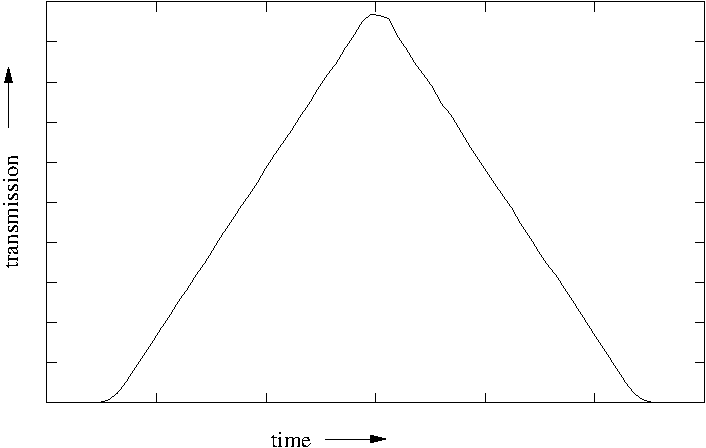
\includegraphics[width=1.0\linewidth]{figures/tracho.eps}
\caption{example transmission curve for the disc chopper\label{f:chopper2}}
\end{figure}

When simulating the chopping of a continuous beam,
most of the neutrons could easily be lost.
To improve efficiency, one can set the flag \verb+IsFirst+, which will
allow every neutron ray to pass the {\bf Chopper}, but modify the
time, $t$, to a time at which it is possible to pass.
This can also be used with TOF-instruments, which often
define the starting time of the neutrons at
the position of the first chopper.
Of course, there should be only one ``first chopper'' in
any simulation.
To simulate frame overlap from a ``first chopper'', one can specify
the number of frames to study by the parameter $n_{\rm pulse}$.
%\input{detector}
%% Emacs settings: -*-mode: latex; TeX-master: "manual.tex"; -*-

\section{Bragg scattering single crystals, monochromators}

In this class of components, we are concerned with elastic Bragg
scattering from single crystals. The Mosaic\_anisotropic component
models a thin mosaic crystal with a single scattering vector
perpendicular to the surface. It is a replacement for the Monochromator
component from previous releases; it uses a better algorithm that works
in some cases where the old component would give wrong results. The
Mosaic\_simple component is similar, but has an isotropic mosaic and
allows a scattering vector that is not perpendicular to the surface. The
Single\_crystal component is a general single crystal sample that allows
the input of an arbitrary unit cell and a list of structure factors, and
also allows anisotropic mosaic and $\Delta d/d$ lattice space variation.

\input{Mosaic_simple.tex}
\subsection{Mosaic\_anisotropic: The crystal with anisotropic mosaic}

The component {\bf Mosaic\_anisotropic} is a modified version of the
Mosaic\_simple component, intended to replace the Monocromator component
from previous releases. It restricts the scattering vector to be
perpendicular to the crystal surface, but extends the Mosaic\_simple
component by allowing different mosaics in the horizontal and vertical
direction.

The code is largely similar to that for Mosaic\_simple, and the
documentation for the latter should be consulted for details. The
differences are mainly due to two reasons:
\begin{itemize}
\item Some simplifications have been done since two of the components of
  the scattering vector are known to be zero.
\item The computation of the Gaussian for the mosaic is done done using
  different mosaics for the two axes.
\end{itemize}

The input parameters for the component Mosaic\_anisotropic are
\textit{zmin}, \textit{zmax}, \textit{ymin}, and \textit{ymax} to define
the size of the crystal (in meters); \textit{mosaich} and \textit{mosaicv} to define
the mosaic (in minutes of arc); \textit{r0} to define the reflectivity
(no unit); and \textit{Q} to set the length of the scattering vector (in
$\mbox{\AA}^{-1}$).

\input{Single_crystal.tex}

\subsection{Monochromator: The monochromator crystal}
The component {\bf Monochromator} is obsolete as from McStas version
1.2. Use the component {\bf Mosaic\_anisotropic} instead.

%\input{powder}
%% Emacs settings: -*-mode: latex; TeX-master: "manual.tex"; -*-

\section{Inelastic scattering kernels}
\label{s:inelastic}

In this section, samples with inelastic scattering are
described. Currently, only a single sample is available that scatters
uniformly in $({\bf Q}, \omega)$ and is used for computing resolution
functions in tripple-axis instruments.

\subsection{Res\_sample: A uniform scatterer for resolution calculation}
\label{s:res_sample}

The component \textbf{Res\_sample} models an inelastic sample that
scatters completely homogeneous in position and energy; regardless of
the state of the incoming neutron, all directions and energies for the
scattered neutron have the same probability. This clearly does not
correspond any physically realizable samples, but the component is very
useful for computation of the resolution function and may also be used
for test and debugging purposes. The component is designed to be used
together with the \textbf{Res\_monitor} component, described in
section~\ref{s:res_monitor}.

The shape of the sample is either a hollow cylinder (like the vanadium
sample described in section~\ref{s:v_sample}) or a rectangular box. The
hollow cylinder shape is specified with inner and outer radius \textit{radius\_i}
and \textit{radius\_o} and height \textit{h}. If \textit{radius\_o} is
negative, the shape is instead a box of width \textit{radius\_i} along
the X axis, height \textit{h}, and thickness $-\textit{radius\_o}$ along the
Z axis, centered on the Z axis and with the front face in the X-Y
plane. See figure~\ref{f:res_sample}.\par
%
\begin{figure}[htbp]
  \begin{center}
        \psfrag{ri}[c][c]{\textit{radius\_i}}
        \psfrag{ro}[c][c]{\textit{radius\_o}}
        \psfrag{h}[c][c]{\textit{h}}
        \psfrag{bri}[c][c]{\textit{radius\_i}}
        \psfrag{bro}[c][c]{$-\textit{radius\_o}$}
        \psfrag{bh}[c][c]{\textit{h}}
        \psfrag{X}[c][c]{\textit{X}}
        \psfrag{Y}[c][c]{\textit{Y}}
        \psfrag{Z}[c][c]{\textit{Z}}
        \includegraphics[width=0.9\textwidth]{figures/res_sample.eps}
    \caption{The two possible shapes of the \textbf{Res\_sample} component.}
    \label{f:res_sample}
  \end{center}
\end{figure}
%
The component only propagates the neutrons that are scattered; neutrons
that would pass through or miss the sample are absorbed. There is no
modeling of the cross section of the sample, secondary extinction
\textit{etc.}; the scattering probability is proportional to the neutron
flight path length inside the sample, with the constant of
proportionality arbitrarily set to $1/(2|\textit{radius\_o}|)$. The
reason for this is that the component is designed for computing the resolution
function of an instrument, including the sample size but independent of
any sample properties such as scattering and absorbtion cross sections.

The point of scattering in the sample is chosen at a random position
along the neutron flight path inside the sample, and the scattered
neutron is given a random energy and direction. The energy is selected in
a user-specified interval $[E_0-\Delta E; E_0+\Delta E]$ which must be
chosen large enough to cover all interesting neutrons, but preferably
not excessively large for reasons of efficiency. Similarly, the
direction is chosen in a user-specified range; the range is such that a
sphere of given center and radius is fully illuminated.

A special feature, used when computing resolution functions, is that the
component stores complete information about the scattering event in the
output parameter \textit{res\_struct}. The information includes initial
and final wave vectors, the coordinates of the scattering point, and the
neutron weight after the scattering event. From this information the
scattering parameters $({\bf Q}_i, \omega_i)$ for every scattering event
$i$ may be recorded and used to compute the resolution function of an
instrument, as explained below. For an example of how to use the
information in the output parameter, see the description of the
\textbf{Res\_monitor} component in section~\ref{s:res_monitor}.

The input parameters to the \textbf{Res\_sample} components are the
sample dimensions \textit{radius\_i}, \textit{radius\_o}, and
\textit{h}, all in meters; the center of the scattered energy range
\textit{E0} and the energy spread \textit{dE} in meV; and the target
sphere position in the local coordinate system \textit{target\_x},
\textit{target\_y}, \textit{target\_z}, and radius \textit{focus\_r}, in
meters. The only output parameter is \textit{res\_struct} containing
information about the scattering event, with all vectors given in the
local coordinate system of the component in units of meter.

\subsubsection{Background}

In an experiment, as well as in the simulation, the expected intensity
is by definition of the resolution function given by
%
$$
  I = \int R({\bf Q}, \omega) \sigma({\bf Q}, \omega) d{\bf Q}d\omega
$$
%
Here $I({\bf Q}_0, \omega_0)$ is the measured or simulated intensity in
the detector, $R$ is the resolution function for the instrument in a
given setup, $\sigma$ is the scattering cross section of the sample, and
$({\bf Q}, \omega)$ denote the scattering vector and energy transfer in
the sample. For the uniform scatterer, $\sigma({\bf Q}, \omega) = 1/V_0$
is a constant, so we have
%
$$
  I = 1/V_0 \int R({\bf Q}, \omega) d{\bf Q}d\omega
$$
%
If we instead consider only the intensity contributed by scattering with
parameters $({\bf Q}, \omega)$ that lie within a small part $\Delta\Omega$ of
the total phase space and has volume $\Delta V$,
%
$$
  I_{\Delta\Omega} = 1/V_0 \int_{\Delta\Omega} R({\bf Q}, \omega) d{\bf Q}d\omega
  = \frac{\Delta V}{V_0} R(\Delta\Omega)
$$
%
(where $R(\Delta\Omega)$ denotes the average value of $R$ over
$\Delta\Omega$), we get a good approximation of the value of $R$
provided that $\Delta\Omega$ is sufficiently small. This is useful with
the output from the simulations, since $I_{\Delta\Omega}$ is
approximated by

$$ I_{\Delta\Omega} \approx \sum_{({\bf Q_i},\omega_i) \in \Delta\Omega} p_i $$


This can be used to
histogram the resolution function or visualize it in different ways. The
3D visualization of the resolution function produced by the
\verb+mcresplot+ program for example uses this by displaying a cloud of
dots, the local density of which is proportional to the resolution
function.

The \verb+mcresplot+ program also computes the covariance and resolution
matrices. Letting $(x^1_i,x^2_i,x^3_i,x^4_i)$ denote the $({\bf
  Q_i},\omega_i)$ values obtained from the scattering events in the
simulation and $\mu^j = (\sum_i p_i x^j_i) / (\sum_i p_i)$ the mean
value of $x^j_i$, the covariance matrix is computed as
$$ {\bf C}_{jk} = \Big(\sum_i p_i (x^j_i - \mu_j) (x^k_i - \mu_k)\Big) /
   \Big(\sum_i p_i\Big) $$
This covariance matrix is given in the local coordinate system of the
sample component. The \verb+mcresplot+ program actually outputs the
covariance matrix in another coordinate system which is rotated around
the Y axis so that the projection to the X-Z plane of the average
scattering vector ${\bf Q}_{\rm avg} = (\sum_i p_i {\bf Q}_i) / (\sum_i
p_i)$ is parallel to the X axis.

The resolution matrix ${\bf M}$ is the inverse of the covariance matrix
and is also output in the rotated coordinate system by \verb+mcresplot+.
The 4-dimensional gaussian distribution, defined by
\begin{equation}
  \label{eq:gauss-res}
  f({\bf X}) = e^{-\frac{1}{2}{\bf X}^T {\bf M} {\bf X}}
\end{equation}
where ${\bf X} = ({\bf Q},\omega)$, has covariance matrix ${\bf C}$ and
thus defines the gaussian resolution function with the same covariance
as the resolution computed by the simulation.

The \verb+mcresplot+ program provides for the simultaneous visualization
of the computed and the gaussian resolution function by obtaining an
appropriate number of random points with the statistical
distribution~(\ref{eq:gauss-res}). Each point ${\bf X}$ is obtained as
follows: A vector ${\bf Y}$ is generated of four individually gaussian
distributed random numbers with mean zero and variance one. Using the
Cholesky decomposition of ${\bf C}$, ${\bf C} = {\bf L}{\bf L}^T$, we
have
$$ {\bf X} = {\bf L} {\bf Y}.$$





% Emacs settings: -*-mode: latex; TeX-master: "manual.tex"; -*-

\chapter{Source components}
\label{c:source}
\index{Sources}
\index{Library!Components!sources}

\MCS\ contains a number of different source components,
and any simulation will contain exactly one source.
The main function of a source is to determine a set of initial
parameters $({\bf r}, {\bf v}, t)$, or equivalent (${\bf r}, v, \Ombold , t $),
for each neutron. This is done by Monte Carlo choices from
suitable distributions. For example, the initial position is
always found from a uniform distribution over the source surface.
For time-of-flight sources, the choice of $t$ is being made on basis of
detailed analytical expressions.
For other sources, the initial neutron time is set to zero (default). In the case you would like to use a 'conventional' source (e.g. steady state source) with time-of-flight settings, it is then \emph{important} to set the time of each neutron using a random number from a distribution. This may be achieved thanks to the \verb+EXTEND+ keyword in the instrument description source:\index{Keyword!EXTEND}

\begin{verbatim}
  TRACE

  COMPONENT MySource=Source_gen(...) AT (...)
  EXTEND
  %{
    t = 1e-3*randpm1(); /* set time to +/- 1 ms */
  %}
\end{verbatim}

Polarization is not relevant for sources,
and we let the neutron spin ${\bf s}=(0,0,0)$.

The shape of most sources can be chosen to be either circular or rectangular.
The initial neutron velocity is selected within an interval
of either the corresponding energy or the corresponding wavelength.

The flux of the sources deserves special attention. The total neutron
intensity is defined as the sum of weights of all emitted neutron rays
during one simulation
(the unit of total neutron weight is thus neutrons per second).
The flux is then defined as intensity per area of the source.
For samples that uses a realistic energy/wavelength distribution,
the neutron intensity is given as the integrated neutron intensity
inside the energy/wavelength range. Similarly, as most sources can focus neutrons to an input window (usually the guide entrance), the intensity is scaled to account for the corresponding solid angle.

The flux~$\Phi$ is the number of neutrons emitted per second from a
one~cm$^2$ area on the source surface, with direction within a one
steradian solid angle, and with wavelength within a one {\AA}ngstr{\o}m
interval. The total number of neutrons emitted towards a given diaphragm
in one second is therefore
$$ N_{\rm total} = \Phi A \Omega \Delta\lambda $$
where $A$ is the source area, $\Omega$ is the solid angle of the
diaphragm as seen from the source surface, and $\Delta\lambda$ is the
width of the wavelength interval in which neutrons are emitted (assuming
a uniform wavelength spectrum). If $N_{\rm sim}$ denotes the number of
neutron histories to simulate, the initial neutron weight $p_0$ must be set to
$$ p_0 = \frac{N_{\rm total}}{N_{\rm sim}} =
    \frac{\Phi}{N_{\rm sim}} A \Omega \Delta\lambda $$

The simulations are performed so that detector intensities
are independent of the number of neutron histories simulated
(though of course more neutron histories will give better statistics).

As a start, we recommand new \MCS\ users to use the Source\_simple component, then use the Source\_Maxwell\_3 or the Source\_gen.

Optimizers can dramatically improve the statistics, but may occasionally give wrong results, due to misleaded optimization. You should always check such simulations with non-optimized ones.

Other ways to speed-up simulations are to read events from a file. See section \ref{sources-seealso} for possible file formats.

\begin{figure}
  \begin{center}
    \includegraphics[width=0.9\textwidth]{figures/sources.eps}
  \end{center}
\caption{A circular source component (at z=0) emitting neutron events randomly, either from a model, or from a data file.}
\label{f:source}
\end{figure}

\newpage
\section{Source\_simple: A simple continuous source
with a flat energy/wavelength spectrum}
\label{source-simple}
\index{Sources!Source\_simple}

\component{Source\_simple}{System}{ $r_{\rm s}$, $z_{\rm foc}$, $w$, $h$, $E_0$, $\Delta E$, $\Psi$}{$\lambda_0$, $d\lambda$}{Validated, position is the center of disk}

This component is
a simple source with a energy distribution which is uniform
in the range $E_0 \pm dE$
(or wavelength distribution in the range $\lambda_0 \pm d\lambda$).
This component is not used for detailed time-of-flight simulations,
so we put $t=0$ for all neutron rays.

The initial neutron ray position is chosen randomly from within a
circle of radius $r_{\rm s}$ in the $z=0$ plane.
This geometry is a fair approximation
of a cylindrical cold/thermal source with the beam going out along
the cylinder axis.

The initial neutron ray direction is focused within
a solid angle, defined by a rectangular target of width
$w$, height $h$, parallel to
the $xy$ plane placed at $(0,0,z_{\rm foc})$.

The initial weight of the created neutron ray, $p_0$, is set to the
energy-integrated flux, $\Psi$, times the source area, $\pi r_{\rm s}^2$
times a solid-angle factor, which is basically the
solid angle of the focusing rectangle.
See also the discussion on focusing in the \MCS\ Manual \ref{s:focus}.

This component replaces Source\_flat, Source\_flat\_lambda,
Source\_flux and Source\_flux\_lambda.


\newpage
\section{Source\_div: A divergent source}

{\bf Source\_div} is a rectangular source which emits a
beam of a certain divergence around the main exit direction
(the direction of the $z$ axis).
The beam intensity and divergence are uniform over
the whole of the source, and the energy distribution
of the beam is uniform.

This component may be used as a simple model of the
beam profile at the end of a guide or at the sample
position.

The input parameters for Source\_div are the source dimensions
$w$ and $h$ (in m), the divergencies $\delta_h$ and $\delta_v$ (FWHM in degrees), 
and the mean energy $E_0$ and the energy spread $dE$ (both in meV).
The neutron energy range is $(E_0-dE; E_0+dE)$. 



\newpage
\section{Source\_Maxwell\_3: A simple continuous source 
with a Maxwellian spectrum}
\label{source-maxwell}
\index{Sources!Source\_Maxwell\_3}

\component{Source\_Maxwell\_3}{System}{ $h$, $w$, $d_{\rm foc}$, $xw$, $yh$, $\lambda_{\rm low}$, $\lambda_{\rm high}$, $I_1$, $T_1$}{$I_2$, $T_2$, $I_3$, $T_3$}

This component is a source with a Maxwellian energy/wavelength distribution 
sampled in the range $\lambda_{\rm low}$ to $\lambda_{\rm high}$.
This component is not used for detailed time-of-flight simulations,
so $t=0$ for all neutron rays.

The initial neutron ray position is chosen randomly from within a
rectangle of area $h \times w$ in the $z=0$ plane. 

The initial neutron ray direction is focused within
a solid angle, defined by a rectangular target of width
$xw$, height $yh$, parallel to 
the $xy$ plane placed at $(0,0,d_{\rm foc})$. 

The energy distribution used is a sum of 1-3 Maxwellians with
temperatures $T_1$ to $T_3$ and integrated intensities $I_1$ to $I_3$.

The initial weight of the created neutron ray, $\pi_1$, is 
calculated in the following way for one single Maxwellian:
The intensity in a small wavelength interval $(\lambda, \lambda+d\lambda)$ is
$ I_1 M(\lambda,T_1) d\lambda $
where 
$M(\lambda,T_1) = 2 \alpha^2 \exp(-\alpha/\lambda^2) / \lambda^5 $ is the normalized Maxwell distribution ($\alpha=949.0 \rm{K \AA}^2/T_1$).
The number of neutrons per second through a focusing window 
of solid angle $\Omega$
from a source of area $A$ within the wavelength interval $\lambda_1$ to
$\lambda_2$ is thus
\begin{equation}
I_{\rm tot} = \Omega A \int_{\lambda_1}^{\lambda_2} I_1 M(\lambda,T_1) d\lambda.
\end{equation}
In a Monte Carlo integration, the observed intensity becomes
\begin{equation}
I_{\rm MC} \approx N_{\rm MC} \int p(\lambda) \pi_1(\lambda) ,
\end{equation}
where $N_{\rm MC}$ is the number of Monte Carlo steps. 
We here choose the wavelength from a uniform distribution between the two
limits, giving $p(\lambda)=1/(\lambda_{\rm high}-\lambda_{\rm low})$.
To fulfill $I_{\rm tot} = I_{\rm MC}$ we need to have
\begin{equation}
\pi_1(\lambda) = \Omega A \delta\lambda I_1 M(\lambda,T_1) / N_{\rm MC} .
\end{equation}

This expression is strictly valid only for $\Omega \ll 1$, 
see also the discussion on focusing in the \MCS\ Manual \ref{s:focus}. 
The expression is easily generalized to a general number of Maxwellians.


\newpage
\section{Source\_gen: A general continuous source}
\label{source-gen}
\index{Sources!An All-in-One continuous source(Source\_gen)}

\component{Source\_gen}{System, E. Farhi}{$w$, $h$, $xw$, $yh$, $E_0$, $\Delta E$, $T_1$, $T_2$, $T_3$, $I_1$, $I_2$, $I_3$ }{$r$, $\lambda_0$, $d\lambda$, $E_{min}$, $E_{max}$, $\lambda_{min}$, $\lambda_{max}$}{Validated for Maxwellian expressions, position is the center of area}

This component is a continuous neutron source (rectangular or circular), which aims at
a square target centered at the beam (in order to improve MC-acceptance
rate). The angular divergence is then given by the dimensions of the
target. Size may be rectangular (dimension $h$ and $w$, or a disk of radius $r$. The wavelength/energy range to emit is specified either using center and half width, or using minimum and maximum boundaries, alternatively for energy and wavelength.
The flux spectrum is specified with the same Maxwellian parameters as in component Source\_Maxwell\_3 (refer to section \ref{source-maxwell}).

Maxwellian parameters for some sources are in the table given below. For some cases, a correction factor (multiply $I$ parameters) should be used to reach measured data.

\begin{table}
  \begin{center}
  {\let\my=\\
    \begin{tabular}{cccccccc}
    \hline
    Source Name & $T_1$ & $I_1$ & $T_2$ & $I_2$ & $T_3$ & $I_3$ & factor \\
    \hline
    PSI cold source & 150.42 & 3.67e11   & 38.74 & 3.64e11    & 14.84& 0.95e11    &\\
    ILL VCS (H1)    & 216.8  & 1.24e13  & 33.9  & 1.02e13   & 16.7 & 3.0423e12 &\\
    ILL HCS (H5)    & 413.5  & 10.22e12  & 145.8 & 3.44e13    & 40.1 & 2.78e13    & *2\\
    ILL Thermal(H2) & 683.7  & 0.5874e13& 257.7 & 2.5099e13 & 16.7 & 1.0343e12 & /2.25\\
    ILL Hot source  & 1695   & 1.74e13   & 708   & 3.9e12     &      &            &\\
    \end{tabular}
    \caption{Flux parameters for Source\_gen and Source\_Maxwell\_3. ILL cold sources data are obtained from \cite{Ageron89}.}
    \label{t:source-params}
  }
  \end{center}
\end{table}

\newpage
% Emacs settings: -*-mode: latex; TeX-master: "manual.tex"; -*-

\section{Source\_adapt: A neutron source with adaptive importance sampling}
\label{s:Source_adapt}
\label{s:source-adapt}
\index{s:source-adapt}
\index{Optimization}

The {\bf Source\_adapt} component is a neutron source that uses adaptive
importance sampling to improve the efficiency of the simulations. It
works by changing on-the-fly the probability distributions from which
the initial neutron state is sampled so that samples in regions that
contribute much to the accuracy of the overall result are preferred over
samples that contribute little. The method can achieve improvements of a
factor of ten or sometimes several hundred in simulations where only a
small part of the initial phase space contains useful neutrons.
On the other side, a warning is in place here regarding potential wrong results using optimization techniques (see section \ref{s:optim} of the \MCS\ user manual). It is highly recommanded in any case to benchmark 'optimized' simulations against non-optimized ones, checking that obtained results are the same, but hopefully with a much improved statistics.

The physical characteristics of the source are similar to those of
Source\_flat (see section~\ref{sourceaim}). The source is a thin
rectangle in the $X$-$Y$ plane with a flat energy spectrum in a
user-specified range. The flux per area per steradian per
{\AA}ngstr{\o}m per second is specified by the user; the total weight of
neutrons emitted from the source will then be the same irrespectively of
the number of neutron histories simulated, corresponding to one second
of measurements.

The initial neutron weight is given by (see
section~\ref{Source_flux_lambda} for details)
$$ p_0 = \frac{N_{\rm total}}{N_{\rm sim}} =
    \frac{\Phi}{N_{\rm sim}} A \Omega \Delta\lambda $$
Here $\Delta\lambda$ is the total wavelength range of the source; since
the spectrum is flat in energy (but not in wavelength), the flux
will actually be different for different energies. A later version of
this component will probably adapt (in a backward-compatible way) a more
sensible way to specify the flux. For now, an energy or wavelength
monitor (see sections~\ref{s:e_monitor} and~\ref{s:L_monitor}) placed
just after the source will show the actual energy-dependent flux.


\subsection{The adaption algorithm}

The adaptive importance sampling works by subdividing the initial
neutron phase space into a number of equal-sized bins. The division is
done on the three dimensions of energy, horizontal position, and
horizontal divergence, using $N_{\rm eng}$, $N_{\rm pos}$, and $N_{\rm
  div}$ number of bins in each dimension, respectively. The total number
of bins is therefore
$$
N_{\rm bin} = N_{\rm eng} N_{\rm pos} N_{\rm div}
$$
Each bin $i$ is assigned a sampling weight $w_i$; the probability of
emitting a neutron within bin $i$ is
$$
P(i) = \frac{w_i}{\sum_{j=1}^{N_{\rm bin}} w_j}
$$
In order to avoid false learning, the sampling weight of a bin is
kept larger than $w_{\rm min}$, defined as
$$
w_{\rm min} = \frac{\beta}{N_{\rm bin}}\sum_{j=1}^{N_{\rm bin}}w_j,\qquad
    0 \leq \beta \leq 1
$$
This way a (small) fraction $\beta$ of the neutrons are sampled
uniformly from all bins, while the fraction $(1 - \beta)$ are sampled in an adaptive way.

Compared to a uniform sampling of the phase space (where the probability
of each bin is $1/N_{\rm bin}$), the neutron weight
must be adjusted by the amount
$$
\pi_i = \frac{1/N_{\rm bin}}{P(i)} =
    \frac{\sum_{j=1}^{N_{\rm bin}} w_j}{N_{\rm bin} w_i}
$$

In order to set the criteria for adaption, the Adapt\_check component is
used (see section~\ref{s:adapt_check}). The source attemps to sample
only from bins from which neutrons are not absorbed prior to the
position in the instrument at which the Adapt\_check component is
placed. Among those bins, the algorithm attemps to minimize the variance
of the neutron weights at the Adapt\_check position. Thus bins that
would give high weights at the Adapt\_check position are sampled more
often (lowering the weights), while those with low weights are sampled
less often.

Let $\pi = p_1/p_0$ denote the ratio between the neutron weight $p_1$ at
the Adapt\_check position and the initial weight $p_0$ just after the
source. For each bin, the component keeps track of the sum $\psi$ of
$\pi$'s as well as of the total number of neutrons $n_i$ from that
bin. The average weight at the Adapt\_source position of bin $i$ is thus
$\psi_i/n_i$.

We now distribute a total sampling weight of $\beta$ uniformly
among all the bins, and a total weight of $(1 - \beta)$ among bins in
proportion to their average weight $\psi_i/n_i$ at the Adapt\_source
position:
$$
w_i = \frac{\beta}{N_{\rm bin}} +
    (1-\beta) \frac{\psi_i/n_i}{\sum_{j=1}^{N_{\rm bins}} \psi_j/n_j}
$$
After each neutron event originating from bin $i$, the sampling weight $w_i$
is updated.

This basic idea can be improved with a small modification. The problem
is that until the source has had the time to learn the right sampling
weights, neutrons may be emitted with high neutron weights (but low
probability). These low probability neutrons may account for a large fraction of
the total intensity in detectors, causing large variances in the
result. To avoid this, the component emits early neutrons with a lower
weight, and later neutrons with a higher weight to compensate. This way
the neutrons that are emitted with the best adaption contribute the most
to the result.

The factor with which the neutron weights are adjusted is given by a
logistic curve
\begin{equation}
  F(j) = C\frac{y_0}{y_0 + (1 - y_0) e^{-r_0 j}}
\end{equation}
where $j$ is the index of the particular neutron history, $1 \leq j
\leq N_{\rm hist}$. The constants $y_0$, $r_0$, and $C$ are given by
\begin{eqnarray}
  y_0 &=& \frac{2}{N_{\rm bin}} \\
  r_0 &=& \frac{1}{\alpha}\frac{1}{N_{\rm hist}}
     \log\left(\frac{1 - y_0}{y_0}\right) \\
  C &=& 1 + \log\left(y_0 + \frac{1 - y_0}{N_{\rm hist}}
     e^{-r_0 N_{\rm hist}}\right)
\end{eqnarray}
The number $\alpha$ is given by the user and specifies (as a fraction
between zero and one) the point at which the adaption is considered
good. The initial fraction $\alpha$ of neutron histories are emitted
with low weight; the rest are emitted with high weight:
$$ p_0(j) =
    \frac{\Phi}{N_{\rm sim}} A \Omega \Delta\lambda
    \frac{\sum_{j=1}^{N_{\rm bin}} w_j}{N_{\rm bin} w_i}
    F(j)
$$
The choice of the constants $y_0$, $r_0$, and $C$ ensure that
$$
\int_{t=0}^{N_{\rm hist}} F(j) = 1
$$
so that the total intensity over the whole simulation will be correct

Similarly, the adjustment of sampling weights is modified so that the
actual formula used is
$$
w_i(j) = \frac{\beta}{N_{\rm bin}} +
    (1-\beta) \frac{y_0}{y_0 + (1 - y_0) e^{-r_0 j}}
     \frac{\psi_i/n_i}{\sum_{j=1}^{N_{\rm bins}} \psi_j/n_j}
$$

\subsection{The implementation}

\component{Source\_adapt}{K. Nielsen}{$x_{min}$, $x_{max}$, $y_{min}$, $y_{max}$, $E0$, $dE$, dist, $xw$, $yh$, $Phi$}{$\alpha$, $\beta$ (plenty, default values are ok)}{not fully validated}

The heart of the algorithm is a discrete distribution $p$. The
distribution has $N$ \emph{bins}, $1\ldots N$. Each bin has a value
$v_i$; the probability of bin $i$ is then $v_i/(\sum_{j=1}^N v_j)$.

Two basic operations are possible on the distribution. An \emph{update}
adds a number $a$ to a bin, setting $v_i^{\rm new} = v_i^{\rm old} +
a$. A \emph{search} finds, for given input $b$, the minimum $i$ such
that
$$ b \leq \sum_{j=1}^{i} v_j. $$
The search operation is used to sample from the distribution p. If $r$
is a uniformly distributed random number on the interval
$[0;\sum_{j=1}^N v_j]$ then $i = {\rm search}(r)$ is a random number
distributed according to $p$. This is seen from the inequality
$$ \sum_{j=1}^{i-1} v_j < r \leq \sum_{j=1}^{i} v_j, $$
from which $r \in [\sum_{j=1}^{i-1} v_j; v_i + \sum_{j=1}^{i-1} v_j]$
which is an interval of length $v_i$. Hence the probability of $i$ is
$v_i/(\sum_{j=1}^N v_j)$.
The update operation is used to
adapt the distribution to the problem at hand during a simulation. Both
the update and the add operation can be performed very efficiently; how
this is achieved will be described elsewhere.

The input parameters for Source\_adapt are
\textit{xmin}, \textit{xmax}, \textit{ymin}, and
\textit{ymax} in meters to set the source dimensions;
\textit{dist}, \textit{xw}, and \textit{yh}
to set the focusing as for Source\_flat (section~\ref{sourceaim}); \textit{E0} and
\textit{dE} to set the range of energies emitted, in meV (the range
will be from $\textit{E0} - \textit{dE}$ to
$\textit{E0} + \textit{dE}$); flux to set the source flux $\Phi$ in ${\rm
  cm}^{-2} {\rm st}^{-1} \textit{\AA} {\rm s}^{-1}$;
$N_{\rm eng}$, $N_{\rm pos}$, and $N_{\rm
  div}$ to set the number of bins in each dimensions; \textit{alpha} and
\textit{beta} to set the parameters $\alpha$ and $\beta$ as described
above; and \textit{filename} to give the name of a file in which to
output the final sampling destribution.

A good general-purpose value for $\alpha$ and $\beta$ is $\alpha = \beta
= 0.25$. The number of bins to choose will depend on the
application. More bins will allow better adaption of the sampling, but
will require more neutron histories to be simulated before a good
adaption is obtained. The output of the sampling distribution is only
meant for debugging, and the units on the axis are not necessarily
meaningful. Setting the filename to \verb+NULL+ disables the output of
the sampling distribution.

As an alternative, you may use the Source\_Optimizer component (see section \ref{source-optimizer}).


\newpage
\section{Moderator: A time-of-flight source}
\label{s:moderator}
\index{Sources!Time of flight pulsed moderator}

\component{Moderator}{System}{$r_s$, $E_0$, $E_1$, $z_f$, $w$, $h$, $\tau_0$, $E_c$, $\gamma$}{}{}
The simple time-of-flight source component {\bf Moderator} resembles
the source component {\bf Source\_flat} described in \ref{sourceaim}.
Like {\bf Source\_flat}, {\bf Moderator} is circular and focuses
on a rectangular target. Further, the initial velocity is chosen
with a linear distribution within an interval, defined by the
minimum and maximum energies, $E_0$ and $E_1$,
respectively.

The initial time of the neutron is determined on basis of a
simple heuristical model for the time dependence of the
neutron intensity from a time-of-flight source.
For all neutron energies, the flux decay is assumed to be exponential,
\begin{equation}
\Psi(E,t) = \exp(-t/\tau(E)) ,
\end{equation}
where the decay constant is given by
\begin{equation}
\tau(E) = \left\{
\begin{array}{cc}
 \tau_0                               & ; E<E_c \\
 \tau_0 / [ 1 + (E-E_c)^2/\gamma^2 ]  & ; E \geq E_c
\end{array}
\right.
\end{equation}

The input parameters for {\bf Moderator} are the source radius, $r_{\rm s}$,
the minimum and maximum energies, $E_0$ and $E_1$ (in meV),
the distance to the target, $z_{\rm f}$, the dimensions of the target,
$w$ and $h$, and the decay parameters
$\tau_0$ (in $\mu$s), $E_c$, and $\gamma$ (both in meV).

\newpage
\input{Source_Optimizer}

\newpage
% Emacs settings: -*-mode: latex; TeX-master: "manual.tex"; -*-

\subsection{Monitor\_Optimizer: Optimization locations for the
  Sour\-ce\_Op\-ti\-miz\-er component}
\label{s:monitoroptimizer}

This component was contributed by Emmanuel Farhi, Institute
Laue-Langevin.

The {\bf Monitor\_Optimizer} component works with the {\bf
  Source\_Optimizer} component. See section~\ref{s:sourceoptimizer}
for usage.

The input parameters for {\bf Monitor\_Optimizer} are the rectangular
shaped opening coordinates $x_{\rm min}, x_{\rm max}, y_{\rm min}$,
$y_{\rm max}$ (in meters), and the name of the associated instance of
the {\bf
  Source\_Optimizer} component used in the instrument description file (one word,
without quotes).


\newpage
\section{Other sources components}
\label{sources-seealso}

There are other ways to define a source.

Pulsed source components are available for new facilities:\index{Sources!Pulsed sources}
\begin{enumerate}
\item SNS ({\bf contrib/SNS\_source})
\item ISIS ({\bf contrib/ISIS\_moderator})
\item ESS (project) ({\bf ESS\_moderator\_long} and {\bf  ESS\_moderator\_short}).
\end{enumerate}

When no model exists (e.g. not a Maxwellian distribution), you may have access to measurement, estimated flux distributions, event files, and - better - to MCNP/Triploli4 neutron event records. The following components are then for you.

\begin{enumerate}
\item{{\bf misc/Virtual\_input} can read a \MCS\ event file (in text or binary format), often bringing a factor 10 speed-up. See section \ref{virtual_input}.}
\item{{\bf contrib/Virtual\_tripoli4\_input} does the same, but from event files (text format) obtained from the \emph{Tripoli4} \cite{tripoli_webpage} reactor simulation program. Such files are usually huge.\index{Sources!Virtual source from Tripoli4}}
\item{{\bf misc/Vitess\_input} can read \emph{Vitess} \cite{vitess_webpage} neutron event binary files.\index{Sources!Virtual source from Vitess}}
\item{{\bf optics/Filter\_gen} reads a 1D distributionb from a file, and may either modify or set the flux according to it.\index{Sources!from 1D table input}}
\item{A component for reading MCNP "PTRAC" records is planed for a next release. Contact us if you wish to participate.}
\end{enumerate}

% Emacs settings: -*-mode: latex; TeX-master: "manual.tex"; -*-

\chapter{Beam optical components:
Arms, slits, collimators, choppers, guides, monochromators}
This chapter contains a number of optical components 
that is used to modify the neutron beam in various ways,
as well as the ``generic'' component {\bf Arm}.

\section{Arm: The generic component}
\label{explain:arm}
\component{Arm}{System}{(none)}{(none)}

The component {\bf Arm} is empty; is resembles an optical bench
and has no effect on the neutron.
The function of this component is only to set up a local 
co-ordinate system within the instrument definition. 
Other components may then be
positioned relative to the arm component
using the \MCS\ meta-language.
The use of arm components in the instrument definitions
is not required but is recommended for clarity.

{\bf Arm} has no input parameters.
An example of the use of this component is given in the 
sample instrument definitions, listed in Appendix \ref{instcode}.



\newpage
\input{slit}

\newpage
\section{Beamstop: A neutron absorbing area}
\label{beamstop}

\component{Beamstop}{System}{$x_{\rm min}$, $x_{\rm max}$, $y_{\rm min}$, $y_{\rm max}$, $r$}{}

The component {\bf Beamstop} can be seen as the reverse of 
the {\bf Slit} component.
It sets up an area at the $z=0$ plane, and propagates the neutrons 
onto this plane (by the kernel call PROP\_Z0).
Neutrons within this area are ABSORB'ed, 
while all other neutrons are unaffected.

By using this beamtop, some neutrons contributing to the background
in a real experiment will be neglected. 
These are the ones that scatter off the side
of the beamstop, or penetrates the absorbing material.
Further, the holder of the beamstop is not simulated.

{\bf Beamstop} can be either circular or rectangular.
The input parameters of {\bf Beamstop} are the four coordinates,
$(x_{\rm min}, x_{\rm max}, y_{\rm min}, y_{\rm max})$
defining the opening of a rectangle, or the radius $r$ of 
a circle, depending on which parameters are specified.


\newpage
\section{Collimator\_linear: The simple Soller blade collimator}
\label{collimator-linear}

\component{Collimator\_linear}{System}{$x_{min}$, $x_{max}$, $y_{min}$, $y_{max}$, $L$, $\delta$ (in deg.)}{}{}

The component {\bf Collimator\_linear}
models a standard linear Soller blade collimator.
The collimator has two identical rectangular openings,
defined like the one in {\bf Slit}. Neutrons not clearing both
openings are ABSORB'ed, see the discussion in \ref{slit}.
The collimating effect is taken care of by employing an ideal
triangular transmission through the collimator, as explained below.
For a more detailed Soller collimator simulation,
taking every blade into accountm , the {\bf Channeled\_guide}
component can be employed, see section~\ref{s:channeled_guide}.

Let $L$ be the length of the collimator blades
and $d$ the distance between them.
Then let $\phi$ be the angle between the
neutron path and the vertical $y-z$ plane along the collimator axis
($\phi$ is also called the {\em horizontal divergence}).
We then define the collimation angle as the maximal allowed
horizontal divergence: $\delta = \tan^{-1}(d/L)$,
see Fig.~\ref{f:collimator}. Neutrons with a horizontal
divergence angle $|\phi| \geq \delta$ will always
hit at least one collimator blade and will thus be ABSORB'ed.
For smaller divergence angles, $|\phi| < \delta$, the fate of the
neutron depends on its exact entry point.
Assuming that a typical collimator has many blades, the
absolute position of each blade perpendicular to the collimator axis
is somewhat uncertain (and also unimportant in most cases).
A simple statistical consideration now shows that the transmission
probability is $T = 1-\tan|\phi|/\tan\delta$.

\begin{figure}
  \begin{center}
    \psfrag{xmin}[c][c]{$x_{\rm min}$}
    \psfrag{xmax}[c][c]{$x_{\rm max}$}
    \psfrag{ymin}[c][c]{$y_{\rm min}$}
    \psfrag{ymax}[c][c]{$y_{\rm max}$}
    \psfrag{delta}[c][c]{$\delta$}
    \includegraphics[width=0.9\textwidth]{figures/collimator.eps}
  \end{center}
\caption{The geometry of a simple Soller blade collimators:
The real Soller collimator, seen from the top (left),
and a sketch of the component {\bf Soller} (right).
The symbols are defined in the text.}
\label{f:collimator}
\end{figure}

We simulate the collimator by transmitting all neutrons with
$|\phi| < \delta$, but adjusting their weight with the amount
\begin{equation}
\pi_i = T = 1-\tan|\phi|/ \tan\delta ,
\end{equation}
while all others are discarded by the kernel call ABSORB.
If $\delta=0$, the collimating effect is disabled,
so that $\pi_i = 1$ whenever the neutron clears the two apertures.


%\newpage
%\section{Filter\_gen: A general filter using a transmission table}
\label{filter-gen}
\index{Optics!Filter}
\index{Sources!from 1D table input}

\component{Filter\_gen}{System}{$x_{min}$, $x_{max}$, $y_{min}$, $y_{max}$, $file$}{$options$}{validated, flat filter}

This component is an ideal flat filter 
that changes the neutron flux according to a 1D input table (text file).

{\bf Filter\_gen} may act as a source ($options$="set") 
or a filter ($options$="multiply", default mode). 
The table itself is a 2 column free format file which accept comment lines. 
The first table column represent wavevector, energy, or wavelength, 
as specified in the $options$ parameter, 
whereas the second column is the transmission/weight modifier.

A usage example as a source would use 
\verb+options="wavelength, set"+, if the first column in the data 
is supposted to be $\lambda$ (in \AA ). 
Another example using the component as a filter would be 
\verb+options="energy, multiply"+ if the first column is $E$ (in meV).

The input parameters are the filter window size 
$x_{min}$, $x_{max}$, $y_{min}$, $y_{max}$, 
the behaviour specification string $options$ and the file to use $file$. 
Additionally, rescaling can be made automatic with the $scaling$ 
and relative $thickness$ parameters.

Some example data files are given with \MCS\ in the 
\verb+MCSTAS/data+ directory as \verb+*.trm+ files for transmission. 

A filter with finite thickness can be simulated by 
surrounding this component with two slits.

\newpage
% Emacs settings: -*-mode: latex; TeX-master: "manual.tex"; -*-

\section{Advanced optical components: mirrors and guides}

This section describes advanced neutron optical
components such as supermirrors and guides.
The first subsection, however, contains 
only a description of the reflectivity of a supermirror.

\subsection{Mirror reflectivity}
\label{s:mirrorreflect}
To compute the reflectivity of the supermirrors, we use an empirical
formula derived from experimental data (see figure~\ref{f:reflectivity}). 
The reflectivity is given by the following formula
\begin{equation}
  R = \left\{
    \begin{array}{ll}
      R_0 & \textrm{if $Q \leq Q_{\rm c}$} \\
      \frac{1}{2}R_0(1 - \tanh[(Q - m Q_{\rm c})/W])(1-\alpha(Q-Q_{\rm c}))
         & \textrm{if $Q > Q_{\rm c}$}
    \end{array}
  \right.
\end{equation}

\begin{figure}
  \begin{center}
    \includegraphics[width=0.6\textwidth]{figures/supermirror.eps}
  \end{center}
\caption{A typical reflectivity curve for a supermirror,
Eq.~(\protect\ref{e:reflectivity}).}
\label{f:reflectivity}
\end{figure}
Here $Q$ is the length of the scattering vector (in \AA$^{-1}$)
defined by
\begin{equation} \label{e:reflectivity}
Q = |{\bf k}_{\bf i} - {\bf k}_{\bf f}| 
  = \frac{m_{\rm n}}{\hbar} |{\bf v}_{\bf i} - {\bf v}_{\bf f}|, 
\end{equation}
$m_{\rm n}$ being the neutron mass. 
The value $m$ is a parameter determined by the mirror materials,
the bilayer sequence, and the number of bilayers.
As can be seen, $R=R_0$ for $Q < Q_{\rm c}$, which is the
critical scattering wave vector for a single layer of the mirror
material. At higher values of $Q$, the reflectivity starts falling
linearly with a slope $\alpha$ until a cut-off at $Q = m Q_{\rm c}$. 
The width of the cut-off is denoted $W$. For the curve in
figure~\ref{f:reflectivity}, the values are
$$ m=4 \qquad R_0=1 \qquad Q_{\rm c} = 0.02\mbox{ \AA}^{-1} \qquad
   \alpha = 6.49\mbox{ \AA} \qquad W=1/300\mbox{ \AA}^{-1} $$
As a special case, if $m=0$ then the reflectivity is zero for all $Q$,
   \textit{ie.} the surface is completely absorbing.

In the components, the neutron weight is adjusted with the amount $\pi_i = R$. 
To avoid spending large amounts of computation time on very low-weight
neutrons, neutrons for which the reflectivity is lower than about
$10^{-10}$ are ABSORB'ed.

\subsection{Mirror: The single mirror}

The component {\bf Mirror} 
models a single rectangular neutron mirror plate. It can
be used to \textit{e.g.}~assemble a complete neutron guide by putting multiple
mirror components at appropriate locations and orientations in the
instrument definition, much like a real guide is build from individual
mirrors.

The mirror is assumed to lie in the first quadrant of the
$x$-$y$ plane, with one corner at $(0,0,0)$. 
If the neutron trajectory intersects the mirror plate, it is
reflected, otherwise it is left untouched. Since the mirror lies in the
$x$-$y$ plane, an incoming neutron with velocity 
${\bf v}_{\rm i} = (v_x,v_y,v_z)$
is reflected with velocity ${\bf v}_{\rm f} = (v_x,v_y,-v_z)$. 
The computation of the reflectivity is handled as detailed in
section~\ref{s:mirrorreflect}.

The input parameters of this component are
the rectangular mirror dimensions $(l, h)$
and the values of $R_0, m, Q_c, W$, and $\alpha$ for the mirror.


\subsection{Guide: The guide section}

The component {\bf Guide} 
models a guide tube consisting of four flat mirrors. The
guide is centered on the $z$ axis with rectangular entrance and exit
openings parallel to the $x$-$y$ plane. The entrance has the dimensions
$(w_1,h_1)$ and placed at $z=0$. The exit is of dimensions $(w_2,h_2)$
and is placed at $z=l$ where $l$ is the guide length. See
figure~\ref{f:guide}. Neutrons not clearing the guide entrance are
ABSORB'ed. For a more general guide simulation, see the Channeled\_guide
component in section~\ref{s:channeled_guide}.

\begin{figure}
  \begin{center}
    \includegraphics[width=0.9\textwidth]{figures/guide1.eps}
  \end{center}
\caption{The geometry used for the guide component.}
\label{f:guide}
\end{figure}

For computations on the guide geometry, we define the planes of the four
guide sides by giving their normal vectors (pointing into the guide)
and a point lying in the plane:
$$
\begin{array}{rclcrcl}
{\bf n}^v_1 &=& (l, 0, {(w_2 - w_1) / 2})
     & & {\bf O}^v_1 &=& (- w_1 / 2, 0, 0) \\
{\bf n}^v_2 &=& (-l, 0, {(w_2 - w_1) / 2})
     & & {\bf O}^v_2 &=& (w_1 / 2, 0, 0) \\
{\bf n}^h_1 &=& (0, l, {(h_2 - h_1) / 2})
     & & {\bf O}^h_1 &=& (0, - h_1 / 2, 0) \\
{\bf n}^h_2 &=& (0, -l, {(h_2 - h_1) / 2})
     & & {\bf O}^h_2 &=& (0, h_1 / 2, 0) \\
\end{array}
$$
In the following, we refer to an arbitrary guide side by its origin
{\bf O} and normal {\bf n}.

With these definitions, the time of intersection of the neutron with a
guide side can be computed by considering the projection onto the
normal:
\begin{equation} 
t_1 = {({\bf O} - {\bf r}_0) \cdot {\bf n} \over {\bf v} \cdot {\bf n}} 
\end{equation}
For a neutron that leaves the guide through the guide exit we have
\begin{equation}
t_2 = {l - z_0 \over v_z} 
\end{equation}
To compute the interaction of the neutron
with the guide, the neutron is initially propagated to the $z = 0$ plane of the
guide entrance. If it misses the entrance, it is ABSORB'ed. Otherwise,
we repeatedly compute the time of intersection with the
four mirror sides and the guide exit. The smallest positive $t$ thus
found gives the time of the next intersection with the guide (or in the
case of the guide exit, the time when the neutron leaves the guide). The
neutron is propagated to this point, the reflection from the side is
computed and the process is repeated until the neutron leaves the guide.

The reflected velocity ${\bf v}_{\rm f}$ of the neutron with incoming velocity
${\bf v}_{\rm i}$ is computed by the formula
\begin{equation}
 {\bf v}_{\rm f} = 
  {\bf v}_{\rm i} 
   - 2{{\bf n} \cdot {\bf v}_{\rm i} \over {|{\bf n}|^2}} {\bf n}
\end{equation}
This expression is arrived at by again considering the projection onto
the mirror normal (see figure~\ref{f:guidereflect}). The reflectivity of the
mirror is taken into account as explained in section~\ref{s:mirrorreflect}.

\begin{figure}
  \begin{center}
    \includegraphics[width=0.5\textwidth]{figures/guide2.eps}
  \end{center}
\caption{Neutron reflecting from mirror. ${\bf v}_{\rm i}$ and 
${\bf v}_{\rm f}$ are the initial and final velocities, respectively,
and {\bf n} is a vector normal to the mirror surface.}
\label{f:guidereflect}
\end{figure}

There are a few optimizations possible here to avoid redundant
computations. Since the neutron is always inside the guide during the
computations, we always have 
$({\bf O} - {\bf r}_0) \cdot {\bf n} \leq 0$. 
Thus $t \leq 0$ if ${\bf v} \cdot {\bf n} \geq 0$, so in this case
there is no need to actually compute $t$. Some redundant computations
are also avoided by utilizing symmetry and the fact that many
components of {\bf n} and {\bf O} are zero.

The input parameters of this component are
the opening sizes of the entry and exit point of the
guide, $(w_1, h_1)$ and $(w_2, h_2)$, respectively,
the guide length, $l$,
and the values of $R_0, m, Q_c, W$, and $\alpha$ for the mirror.


\subsection{Channeled\_guide: A guide section component with multiple channels}
\label{s:channeled_guide}

The component Channeled\_guide is a more flexible variation of the Guide
component described in the previous section. It allows the specification
of different supermirror parameters for the horizontal and vertical
mirrors, and also implements guides with multiple channels as used in
neutron bender devices. By setting the $m$ value of the supermirror
coatings to zero, nonreflecting walls are
simulated; this may be used to simulate a Soller collimator.

The channel walls are assumed to be infinitely absorbing. The
implementation is basen on that of the Guide component. Initially, the
channel which the neutron will enter is computed. The $x$ coordinate is
then shifted so that the channel can be simulated as a single instance
of the Guide component. Finally the coordinates are restored when the
neutron exits the guide or is absorbed.

The input parameters are \textit{w1}, \textit{h1}, \textit{w2},
\textit{h2}, and \textit{l} to set the guide dimensions in meters as for
the Guide component (entry window, exit window, and length); \textit{k}
to set the number of channels; \textit{d} to set the thickness of the
channel walls, in meters; and \textit{R0}, \textit{W}, \textit{Qcx},
\textit{Qcy}, \textit{alphax}, \textit{alphay}, \textit{mx}, and \textit{my} to
set the supermirror parameters as described above (the names with \textit{x}
denote the vertical mirrors, and those with \textit{y} denote the horizontal
ones).


\newpage
% Emacs settings: -*-mode: latex; TeX-master: "manual.tex"; -*-

\section{Chopper: The disc chopper}
\label{s:chopper}
\index{Optics!Disc chopper}

\component{Chopper}{Phillipp Bernhardt}{$w$, $R$, $f$, $n$, $\phi$}{IsFirst, $n_{\rm pulse}$}{}

To cut a continuous neutron beam into short pulses, or to control
the pulse shape from a pulsed source, one can use a disc
chopper (see figure~\ref{f:chopper1}). This is a fast rotating disc with the
rotating axis parallel to the neutron beam. The disk consists of neutron
absorbing materials. To form the pulses the disk has openings through which
the neutrons can pass.

\begin{figure}[ht]
\includegraphics[width=1.0\linewidth]{figures/Chopper.eps}
\caption{disc chopper\label{f:chopper1}}
\end{figure}

Component {\bf Chopper} has $n$ openings, which are
symmetrically positioned on the disc. You can set the direction of
rotation, which allows to simulate double choppers. You can also define
the phase by setting the time at which one slit is positioned at the
top. The sides of the slits are pointing towards the center of the disc.
The thickness of the disc is neglected.  There is no parameter for the
size of the slits in the radial direction;
use e.g. a {\bf Slit} component in front of the chopper.

Using a rectangular shaped beam with nearly the same
size as the slit, yields an almost triangular shaped
transmission curve (see figure~\ref{f:chopper2}).

\begin{figure}[ht]
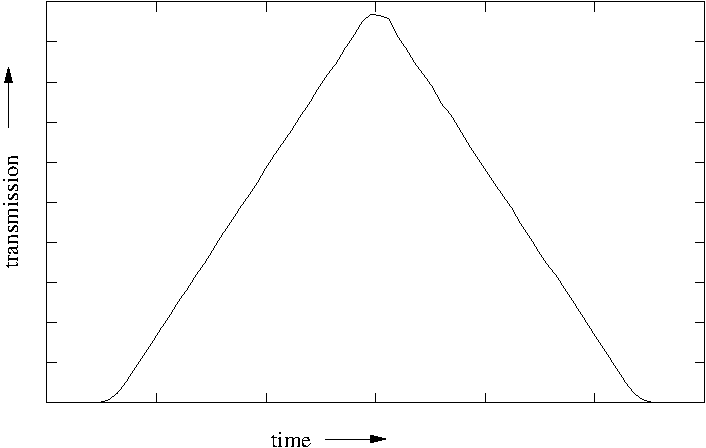
\includegraphics[width=1.0\linewidth]{figures/tracho.eps}
\caption{example transmission curve for the disc chopper\label{f:chopper2}}
\end{figure}

When simulating the chopping of a continuous beam,
most of the neutrons could easily be lost.
To improve efficiency, one can set the flag \verb+IsFirst+, which will
allow every neutron ray to pass the {\bf Chopper}, but modify the
time, $t$, to a time at which it is possible to pass.
This can also be used with TOF-instruments, which often
define the starting time of the neutrons at
the position of the first chopper.
Of course, there should be only one ``first chopper'' in
any simulation.
To simulate frame overlap from a ``first chopper'', one can specify
the number of frames to study by the parameter $n_{\rm pulse}$.

%\newpage
%\input{chopper_fermi}

\newpage
\section{V\_selector: A rotating velocity selector}
\label{vselector}
\index{Optics!Velocity selector}

\component{V\_selector}{System}{$L_0$, $L_1$, $\omega$, $r_0$, $\phi$, $N$}{}{validated, position is center of input aperture}

\begin{figure}
  \begin{center}
    \includegraphics[width=0.9\textwidth]{figures/vselector.eps}
  \end{center}
\caption{A velocity selector}
\label{f:vselector}
\end{figure}

The component {\bf V\_selector} models a rotating velocity
selector constructed from a number of collimator blades
arranged radially on an axis. Two identical slits
at a 12 o'clock position allow
neutron passage at the position of the blades.
The blades are "twisted" on the axis so that a stationary
velocity selector does not transmit any neutrons; the total
twist angle is denoted $\phi$.
By rotating the selector you allow
transmittance of neutrons around certain velocities, given by
\begin{equation}
V_0 = \omega L / \phi ,
\end{equation}
which means that the selector has turned the twist angle
$\phi$ during the neutron flight time $L/V_0$.

Neutrons having a velocity slightly smaller or larger than $V_0$
will either be transmitted or absorbed depending on the exact position
of the rotator blades when the neutron enters the selector.
Assuming this position to be unknown (and assuming infinitely
thin blades), we arrive at
\begin{equation}
T = \left\{
 \begin{array}{ll}
 1 - (N/2\pi ) |\phi-\omega L / V| &
        {\rm if}\,  -1 < (N/2\pi )(\phi -\omega L / V) < 1 \\
    0  &  {\rm otherwise}
 \end{array} \right.
\end{equation}
where $N$ is the number of collimator blades.

A horisontal divergence changes the above formula because of the
angular difference between the entry and exit points of the neutron.
The resulting transmittance resembles the one above, only with
$V$ replaced by $V_z$ and $\phi$ replaced by $(\phi +\psi )$,
where $\psi$ is the angular difference due to
the divergence. An additional vertical divergence does not change
this formula, but it may contribute to $\psi$.
(We have here ignored the very small non-linearity of $\psi$ along the
neutron path in case of both vertical and horisontal divergence).

Adding the effect of a finite blade thickness, $t$, reduces the transmission
by the overall amount
\begin{equation}
dT = (N t) / (2\pi r ) ,
\end{equation}
where $r$ is the distance from the rotation axis. We ignore the variation
of $r$ along the neutron path and use just the average value.

The input parameters for V\_selector are the slit dimensions,
\textit{width}, \textit{height} (in m),
the distance between apertures, $L_0$ (in m), the length of the
collimator blades, $L_1$ (in m), the height from rotation axix to the slit
centre, $r_0$ (in m), the rotation speed $\omega$ (in rpm)
the twist angle $\phi$ (in degrees), the blade thickness $t$ (in m),
and the number of blades, $N$.

The local coordinate system is centered at the slit centre.
The component Selector produces equivalent results.



\newpage
% Emacs settings: -*-mode: latex; TeX-master: "manual.tex"; -*-

\chapter{Monochromators}

In this class of components, we are concerned with elastic Bragg
scattering from monochromators. {\bf Monochromator\_flat} 
models a flat thin mosaic crystal with a single scattering vector
perpendicular to the surface.  
The component {\bf Monochromator\_curved} is physically similar, 
but models a singly or doubly bend monochromator crystal arrangement.

A much more general model of scattering from a single crystal is 
found in the component {\bf Single\_crystal},
which is presented under Samples, chapter~\ref{c:samples}.

\input{monochromator_flat.tex}
\newpage
\input{monochromator_curved.tex}



% Emacs settings: -*-mode: latex; TeX-master: "manual.tex"; -*-

\chapter{Samples}
\index{Library!Components!samples}

This class of components models the sample of the experiment.
This is by far the most challenging part of a neutron scattering
instrument to model. However, for purpose of simulating
instrument performance, details of the samples are rather unimportant,
allowing for simple approximations. On the contrary, for full
virtual experiments it is of importance to have realistic and
detailed sample descriptions. \MCS\ contains both simple and detailed
samples, although there is still room for much more development.

We first consider incoherent scattering. The simple component {\bf Vanadium}
performs both incoherent scattering and absorption.

An important component class is elastic Bragg scattering from an ideal powder.
The components {\bf Powder1} and {\bf Powder2} model a simple powder with one or two
reflections and incoherent scattering. Finally, the {\bf PowderN} component extends the capabilities to N lines, read from a LAZY/Crystallographica data file.

Next type is Bragg scattering from single crystals.
The simplest single crystals are in fact the monochromator components
{\bf Monochromator\_flat} and {\bf Monochromator\_curved},
which were presented in the section on optics.
The monochromators are models of a thin mosaic crystal
with a single scattering vector perpendicular to the surface.
Much more advanced, the component {\bf Single\_crystal}
is a general single crystal sample (with multiple scattering) that allows
the input of an arbitrary unit cell and a list of structure factors, and
also allows anisotropic mosaic and $\Delta d/d$ lattice space variation.

Isotropoic small-angle scattering is simulated in {\bf Sans\_Spheres},
which models scattering from a collection of hard spheres. A more general
SANS sample is highly wanted. In addition, a reflectometry sample
should be developed.

Inelastic scattering from a dispersion is exemplified by
the relatively simple component {\bf Phonon}.

For a more general sample model, the {\bf Isotropic\_Sqw} component is able to simulate all kinds of isotropic materials: liquids, glasses, polymers, powders, ... Physical processes include coherent/incoherent scattering, both elastic and inelastic, with absorption and multiple scattering. Moreover, this compoennt may be used concentrically, to model a sample environment. Thus it may handle most samples except single crystals.

In general, all samples are assumed to be homogeneous. There would also be
potential in developing an inhomogeneous sample, e.g. with
spatially varying lattice constant, relevant for stress/strain scanners.
Inhomogeneously absorbing sample for tomography could also be possible.
Further, no polarization effects are yet taken into account in any
of the samples.

\begin{table}
  \begin{center}
  {\let\my=\\
    \begin{tabular}{|c|cc|cc|c|c|}
    \hline
    Sample        & \multicolumn{2}{c|}{Coherent} & \multicolumn{2}{c|}{Incoherent} &&\\
    Process       & Elastic & Inelastic & Elastic & Inelastic & Absorption & Multi. Scatt.\\
    \hline
    Phonon\_simple&         & X         &         &           & X & \\
    Isotropic\_Sqw&  X      & X         & X       & X         & X & X \\
    Powder1       &  1 line &           &         &           & X & \\
    PowderN       &  N lines&           &         &           & X & \\
    Sans\_spheres &  colloid&           &         &           & X & \\
    Single\_crystal& X      &           & X       &           & X & X \\
    V\_sample     &         &           & X       &           & X & \\
    \hline
    \end{tabular}
    \caption{Processes implemented in sample components}
    \label{t:sample-process}
  }
  \end{center}
\end{table}

\input{vanadium.tex}
\input{powder2.tex}
\input{Single_crystal.tex}
\section{Sans\_spheres: A sample of hard spheres for small-angle scattering}
\label{sans}
\index{Samples!Dilute colloid medium}
\index{Diffraction}
\index{Small angle scattering}

\component{Sans\_spheres}{(System); Lise Arleth, Veterinary University of Denmark}{$R$, $x_w$, $y_h$, $z_t$, $r$, $\sigma_a$}{$phi$, $q_{max}$, $\Delta \rho$}{}

The component {\bf Sans\_spheres} models a sample of small independent
spheres of radius $R$, which are uniformly distributed
in a rectangular volume $x_w \times y_h \times z_t$ with a volume
fraction $\phi$. The absorption cross section density for the spheres
(or is it from the solution?)
is $\sigma_a$ (in units of m$^{-1}$), specified
for neutrons at 2200 m/s. Absorption and incoherent scattering from the medium
is neglected.
The difference in scattering length density
(the contrast) between the hard spheres and the medium is called $\Delta \rho$.
$q_{\rm max}$ denotes the maximum scattered $q$-value that is probed
in the simulation.

\subsection{Small-angle scattering cross section}
The neutron intensity scattered in a solid angle $\Delta \Omega$
for a flat transmission isotropic SANS sample is given by \cite{ILLblue}:
\begin{equation}
I_s(q) = \Psi \Delta\Omega T A z_{\rm max} \frac{d\sigma_v}{d\Omega}(q) ,
\end{equation}
where $\Psi$ is the neutron flux, $T$ is the sample transmission,
$A$ is the illuminated sample area, and $z_{\rm max}$ the length of
the neutron path through the sample.

In this component, we consider only scattering from a thin solution
of monodisperse hard spheres of radius $R$, where the volume-specific
scattering cross section is given by \cite{ILLblue}
\begin{equation}
\frac{d\sigma_v}{d\Omega}(q) =
  n (\Delta\rho)^2 V^2 \left( 3\frac{\sin(qR)-qR\cos(qR)}{(qR)^3} \right)^2 .
\end{equation}
Here, $n$ is the number density of spheres, and $V$ is the
sphere volume. Their product gives the input parameter, $\phi=nV$.

\subsection{Algorithm}
All neutrons, which hit the sample volume, are scattered.
(Hence, no direct beam is simulated.)
For scattred neutrons, the following steps are taken:
\begin{enumerate}
\item Choose a value of $q$ uniformly in the interval $[0;q_{\rm max}]$.
\item Choose a polar angle, $\alpha$,
  for the {\bf q}-vector uniformly in $[0;\pi]$.
\item Scatter the neutron according to $(q,\alpha)$.
\item Calculate and apply the correct weight factor correction.
\end{enumerate}

% Emacs settings: -*-mode: latex; TeX-master: "manual.tex"; -*-


\section{Phonon\_simple: A simple phonon sample}
\label{s:phonon_simple}
\index{Samples!Isotropic acoustic phonon}
\index{Inelastic scattering}

\component{Phonon\_simple}{Kim Lefmann}{ $r_{\rm o}$, $h$, $r_{\rm foc}$, $x_{\rm target}$, $y_{\rm target}$, $z_{\rm target}$, $\sigma_{\rm abs}$, $\sigma_{\rm inc}$, $a$, $b$, $M$, $c$, $DW$, $T$}{$w_x$, $h_y$, $t_z$, $w_{\rm focus}, h_{\rm focus}$, $w_{\rm foc, angle}$, $h_{\rm foc, angle}$, target\_index}{}
\input{phonon_extra.tex}

\section{Isotropic\_Sqw: A general $S(q,\omega)$ coherent and incoherent scatterer}
\label{s:isotropic-sqw}
\index{Samples!Coherent and incoherent isotropic scatterer}
\index{Coherent and incoherent isotropic scatterer}
\index{Inelastic scattering}

\component{Isotropic\_Sqw}{V. Hugouvieux, E. Farhi}{Sqw$\_{coh}$, $\sigma_{coh}$, Sqw$\_{inc}$, $\sigma_{inc}, V_\rho, \sigma_{abs}, T$}{$q_{min}, q_{max}, \omega_{min}, \omega_{max}, d\phi$, order}{not fully validated}

\begin{figure}
  \begin{center}
    \includegraphics[width=0.9\textwidth]{figures/sqw.eps}
  \end{center}
\caption{An $l-^4$He sample in a cryostat, simulated with the Isotropic\_Sqw component in concentric geometry.}
\label{f:isotropic-sqw}
\end{figure}

The component assumes that the sample has the structure of a liquid. This stands for indeed normal liquids, glasses (amorphous systems), polymers, and may be extended to powders.

\subsection{A short introduction to the theory of liquids}

\begin{figure}
  \begin{center}
    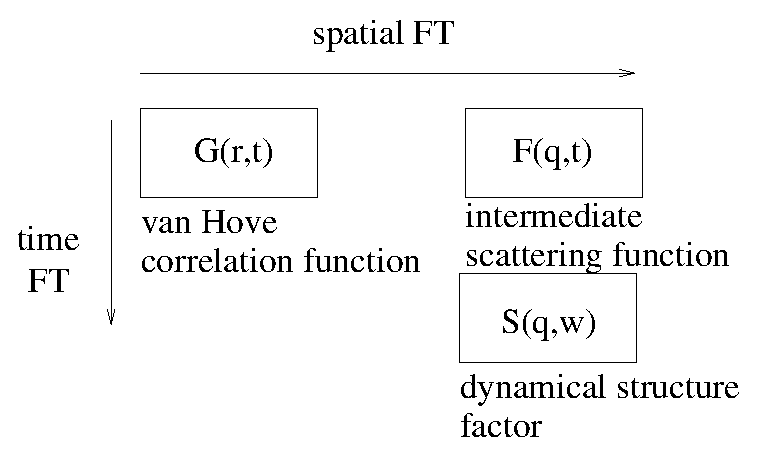
\includegraphics[width=0.9\textwidth]{figures/GFS.eps}
  \end{center}
\caption{Relations between dynamical functions using space, time, wavevector and energy variables.}
\label{f:GFS}
\end{figure}

In the case of a homogeneous and classical liquid, the \emph{van Hove correlation function}, which describes the time and space correlations in the liquid, can be written \cite{Egelstaff67,squires}:
\begin{equation} \label{eq:vanhove}
G(\vec{r},t) = \frac{1}{N} \sum_{i=1}^N \sum_{j=1}^N  \langle\delta[\vec{r} + \vec{r}_i(0) - \vec{r}_j(t)]\rangle
\end{equation}
with $\vec(r)$ and $t$ being the position and time of the atom distribution in the liquid.
Using the particule-density function $\rho(\vec(r),t)$, the function $G$ can be rewritten:
\begin{equation} \label{eq:vanhove-rho}
G(\vec{r},t) = \frac{\langle \rho(0,0) \rho(\vec{r},t)\rangle}{\rho}
\end{equation}

On the experimental point of view, one usually refers to the \emph{dynamical structure factor} $S(q,\omega)$, which is the double Fourier-transform in space and time of the van Hove correlation function $G(r,t)$:
\begin{eqnarray} \label{eq:sqw-rho}
S(q,\omega) &= \frac{1}{2\pi}\int_{-\infty}^{\infty} F(\vec{q},t) e^{-i\omega t} dt \nonumber \\
            &= \frac{1}{2\pi N} \int_{-\infty}^{\infty} \langle \hat\rho^*(\vec{q},0) \hat\rho(\vec{q},t) \rangle e^{-i\omega t} dt.
\end{eqnarray}
where $\hat\rho(\vec{q}, t)$ is the spatial Fourier transform of the density $\rho(\vec{r},t)$, and the \emph{intermediate scattering function} $F$ is the time correlation function of $\hat\rho$:
\begin{eqnarray}
F(\vec{q},t) &= \frac{1}{N} \langle \hat\rho^*(\vec{q},0)  \hat\rho(\vec{q},t) \rangle \nonumber \\
                    &= \frac{1}{N} \sum_{i=1}^N \sum_{j=1}^N \langle e^{i \vec{q}.(\vec{r}_j(t) - \vec{r}_i(0))} \rangle
\end{eqnarray}
Some easely measureable quantities in a liquid are the \emph{pair correlation function} $g(r)$ and the \emph{structure factor} $S(q)$, defined as:
\begin{eqnarray}
\rho g(\vec{r}) &= \frac{1}{N} \sum_{i=1}^N \sum_{j \neq i} \langle \delta(\vec{r}+\vec{r}_i-\vec{r}_j) \rangle \\
S(\vec{q}) &=1 + \rho \int_V [g(\vec{r})-1] e^{i\vec{q}.\vec{r}} d\vec{r} \\
           &=1 + \rho \int_{0}^{\infty} [g(r)-1] \frac{\sin(qr)}{qr} 4 \pi r^2 dr {\rm in isotropic materials}
\end{eqnarray}
Both $g(r)$ and $S(q)$ converge to unity for large $r$ and $q$ values respectively, and they are representative of the atoms spatial distribution.


Following Squires (\cite{squires}, p63), the neutron differential scattering cross section for both coherent and incoherent processes is
\begin{equation}
\frac{d^2\sigma}{d\Omega dE_f} = \frac{\sigma}{4\pi}\frac{k_f}{k_i} N S(q, \omega)
\end{equation}
with usual notations. The unit of the dynamical structure factor $S$ is an inverse energy.

\subsection{How does a neutron interact with the material ?}


\subsection{The implementation}
\subsubsection{Choosing the interaction position}
\subsubsection{Choosing the type of interaction}
\subsubsection{Choosing the $q$ and $\omega$ transfert}
%\input{LSCO.tex}


% Emacs settings: -*-mode: latex; TeX-master: "manual.tex"; -*-

\chapter{Monitors and detectors}

In real neutron experiments, detectors and monitors play quite
different roles. One wants the detectors to be as efficient as 
possible, counting all neutrons (absorbing them in the process), 
while the monitors measure the intensity of the incoming beam, and must
as such be almost transparent, interacting only with (roughly) 0.1-1\%
of the neutrons passing by. In computer simulations, it is 
of course possible to detect every neutron without 
absorbing it or disturbing any of its parameters. Hence, the two components
have very similar functions in the simulations, and we do
not distinguish between them. For simplicity, they are from here on
just called monitors, since they do not absorb neutrons.

Another important difference between computer simulations 
and real experiments is
that one may allow the monitor to be sensitive to any neutron property,
as {\em e.g.} direction, energy, and divergence, in addition to what
is found in advanced existing monitors (space and time). One may, in
fact, let the monitor have several of these properties at the same time,
as seen for example in the energy sensitive monitor in
section~\ref{s:e_monitor}.

When a monitor detects a neutron ray, 
a number counting variable is incremented: $n_i = n_{i-1}+1$
In addition, the neutron
weight $p_i$ is added to the weight counting variable:
$I_i = I_{i-1} + p_i$, 
and the second moment of the weight is
updated: $M_{2,i} = M_{2,i-1} + p_i^2$. 
As also discussed in the System Manual, after a simulation of $N$ rays
the detected intensity (in units of neutrons/sec.) is $I_N$,
while the estimated errorbar is $\sqrt{M_{2,i}^2}$.


Many different monitor components have been developed for
\MCS , but we have selected to support only the most important ones.
One example of the monitors we have omitted is the single monitor,
{\bf Monitor},
that measures just one number (with errorbars) per simulation.
This effect is mirrored by any of the 1- or 2-dimensional detectors
we support, e.g. the {\rm PSD\_monitor}. 
In case additional functionality of monitors is required,
the existing monitors can easily be modified.
However, the ultimate solution is the use of the 
``Swiss army knife'' of monitors, {\rm Monitor\_nD}, that can face
almost any simulation challenge. 

\newpage
% Emacs settings: -*-mode: latex; TeX-master: "manual.tex"; -*-

\section{TOF\_monitor: The time-of-flight monitor}
\component{TOF\_monitor}{System}{$x_{\rm min}$, $x_{\rm max}$, $y_{\rm min}$, $y_{\rm max}$, $n_{\rm chan}$, $t_0$, $t_1$, filename}{$\Delta t$}

The component {\bf TOF\_monitor} has a rectangular opening
in the $x-y$ plane, given by the $x$ and $y$ parameters,
like for {\rm Slit}. 
The neutron is propagated to the plane of the monitor
by the kernel call PROP\_Z0.
Any neutron ray that passes within the opening is counted, and
the total neutron counts are updated:

Special about {\bf TOF\_monitor} is that it is sensitive to
the time, $t$, where the neutron ray is hits the component.
Like in a real time-of-flight detector, the time dimension is
binned into small time intervals. 
Hence this monitor updates a one-dimensional array of counts.
The $n_{\rm chan}$ time intervals begin at $t_0$ and 
end at $t_1$ (or have each length $dt$ if this parameter is specified). 
As usual in time-of-flight analysis, all times are given in units of $\mu$s.

The output parameters from {\bf TOF\_monitor} are the three count numbers, 
$N, I$, and $M_2$ for the total counts in the monitor.
In addition a file is produced with a list of the same three data divided in
different TOF bins.
This file can be read and plotted by the {\rm MCplot} tool; see the
System Manual.



\newpage
% Emacs settings: -*-mode: latex; TeX-master: "manual.tex"; -*-

\section{E\_monitor: The energy-sensitive monitor} \label{s:e-monitor}
\index{Monitors!Energy monitor}
\component{E\_monitor}{System}{$x_{\rm min}$, $x_{\rm max}$, $y_{\rm min}$, $y_{\rm max}$, $n_{\rm chan}$, $E_{\rm min}$, $E_{\rm max}$, filename}{}{}

The component {\bf E\_monitor} resembles {\bf TOF\_monitor}
to a very large extent. Only this monitor is sensitive to
the neutron energy, which in binned in \textit{nchan} bins between
$E_{\rm min}$ and $E_{\rm max}$.

The output parameters from {\bf E\_monitor} are the total counts,
and a file with 1-dimensional data vs. $E$, similar to {\bf TOF\_monitor}.




\newpage
\input{l_monitor}

\newpage
% Emacs settings: -*-mode: latex; TeX-master: "manual.tex"; -*-

\section{PSD\_monitor: The PSD monitor}
\component{PSD\_monitor}{System}{$x_{\rm min}$, $x_{\rm max}$, $y_{\rm min}$, $y_{\rm max}$, $n_x$, $n_y$, filename}{}


The component {\bf PSD\_monitor} resembles other monitors, e.g. 
{\bf E\_Monitor}, and also propagates the neutron to the detector
surface in the $(x,y)$-plane, where the detector window is set
by the $x$ and $y$ input coordinates.
The PSD monitor, though, is not sensitive to the neutron energy, but
rather its position. the rectangular monitor window is divided
into $n_x \times n_y$ pixels, each of which acts like a single
counter.

The output from {\bf PSD\_monitor} is the integrated counts, $n, I, M_2$, 
as well as 
three two-dimensional arrays of counts: $n(x,y), I(x,y), M_2(x,y)$.
The arrays are written to a file and can be read e.g. by the tool
{\bf MC\_plot}, see the system manual.

{\bf Burde man ikke kunne specificere en radius, 
og s\aa\ blev den en 2D cylinder detektor??}

\newpage
\input{div_monitor}

\newpage
\input{divpos_monitor}

%\newpage
%\input{monitor_nd}
\chapter{Special-purpose components}
\index{Library!Components!misc}

The chapter deals with components that are not easily included
in any of the other chapters because of their special nature,
but which still are considered to be of significant importance
to \MCS .

One part of these components deals with splitting simulations
into two (or more) stages. For example, a guide system is often
not changed much, and a long simulation of neutron rays
``surviving'' through the guide system could be reused
for several simulations of the instrument back-end, speeding up
the simulations by (typically) one or two orders of magnitude.
The components for doing this trick is {\bf Virtual\_input} and
{\bf Virtual\_output}, which stores and reads neutron rays, respectively.

Another pair of components performs the simulation of the instrument
resolution functions. This is {\bf Res\_sample}, that is to be
placed at the sample position, and {\bf Res\_monitor}, that should
be localized at the position of the instrument detector.

\newpage
\section{Vitual\_input: Starting the second part of a split simulation}
\label{virtual_input}

\component{Virtual\_input}{System}{filename}{buffer size, repeat count, type}

The component {\bf Virtual\_input} resumes a split simulation where the 
first part has been performed by another instrument and the neutron ray
parameters have been stored by the component {\bf Virtual\_output}.

All neutron ray parameters are read from the input file, which is by default
of ``text'' type, but can also assume the binary formats 
``float'' or ``double''. The reading of neutron rays continue until the 
specified number of rays have been simulated or 
till the file has been exhausted. If desirable, the input file
can be reused a number of times, determined by the optional parameter
``repeat count''. However, care should be taken when dealing with 
absolute intensities, which are automatically correct only
when the input file has been exhausted once.

For performance reasons, it is possible to specify the size of 
the buffer to use in reading the neutron rays from file. Default 
is to buffer the whole file, but this may be fatal for very large
input files.

\section{Vitual\_output: Saving the first part of a split simulation}
\label{virtual_output}

\component{Virtual\_output}{System}{filename}{buffer size, type}

The component {\bf Virtual\_output} stores the neutron ray parameters
from a split simulation. It is then possible to let the 
next part of the simulation be performed by another instrument,
which reads the stored neutron ray
parameters by the component {\bf Virtual\_input}.

All neutron ray parameters are saved to the output file, which is by default
of ``text'' type, but can also assume the binary formats 
``float'' or ``double''. The storing of neutron rays continue until the 
specified number of simulations have been performed.

For performance reasons, it is possible to specify the size of 
the buffer to use in writing the neutron rays to file. Default 
is to buffer the whole file, but this may be fatal for very large
simulations.


\newpage
% Emacs settings: -*-mode: latex; TeX-master: "manual.tex"; -*-

\section{Res\_sample: A uniform scatterer for resolution calculation}
\label{s:res_sample}
\index{Samples!Resolution function, sample for}

\component{Res\_sample}{System, Alan Tennant}{$r_{\rm i}$, $r_{\rm o}$, $h$, $r_{\rm focus}$, $x_{\rm target}$, $y_{\rm target}$, $z_{\rm target}$, $E_0$, $\Delta E$ }{$x_w$, $y_h$, $z_t$, $x_{\rm focus}$, $y_{\rm focus}$, $a_{\rm v, focus}$, $a_{\rm h, focus}$, target index}{}

The component \textbf{Res\_sample} models an inelastic sample that
scatters completely homogeneous in position and energy,
within specified intervals. Regardless of
the state of the incoming neutron, all directions and energies for the
scattered neutron have the same probability. This is clearly
not a physical sample! Rather, the component is meant
for computation of the resolution function, but it may also be used
for test and debugging purposes. For calculations of the resolution
function, {\bf Res\_sample} should be used
together with the \textbf{Res\_monitor} component, described in
section~\ref{s:res_monitor}.

The shape of {\rm Res\_sample} is either a hollow cylinder
or a rectangular box, as specified for {\rm Vanadium}
(see section~\ref{s:v_sample}).The hollow cylinder shape is
specified with the inner and outer radius, $r_{\rm i}$ and $r_{\rm o}$,
respectively, and the height, $h$.
If these parameters are unspecified,
the shape is instead a box of dimensions $x_w$, $y_h$, and $z_t$.
See figure~\ref{f:res_sample}.\par
%
\begin{figure}[htbp]
  \begin{center}
        \psfrag{ri}[c][c]{\textit{radius\_i}}
        \psfrag{ro}[c][c]{\textit{radius\_o}}
        \psfrag{h}[c][c]{\textit{h}}
        \psfrag{bri}[c][c]{\textit{radius\_i}}
        \psfrag{bro}[c][c]{$-\textit{radius\_o}$}
        \psfrag{bh}[c][c]{\textit{h}}
        \psfrag{X}[c][c]{\textit{X}}
        \psfrag{Y}[c][c]{\textit{Y}}
        \psfrag{Z}[c][c]{\textit{Z}}
        \includegraphics[width=0.9\textwidth]{figures/res_sample.eps}
    \caption{The two possible shapes of the \textbf{Res\_sample} component.}
    \label{f:res_sample}
  \end{center}
\end{figure}
%
The component only propagates the neutrons that are scattered; neutrons
that would pass through or miss {\bf Res\_sample} are absorbed. There is no
modeling of the cross section of the sample, secondary extinction
\textit{etc.}; the scattering probability is proportional to the neutron
flight path length inside the sample, with the constant of
proportionality arbitrarily set to $1/(2|\textit{radius\_o}|)$. The
reason for this is that the resolution
function of an instrument (although including the sample size)
is independent of any sample properties such as scattering
and absorbtion cross sections.does not depend on the scattering
cross section.

The point of scattering in the sample is chosen uniformly
along the neutron flight path inside the sample, and the scattered
neutron is given a random energy and direction. The energy is selected in
the interval $[E_0-\Delta E; E_0+\Delta E]$ which hence must be
chosen large enough to cover all interesting neutrons. Similarly, the
direction is chosen in a user-specified range,
either within a sphere of radius $r_{\rm foc}$, within a rectangular
target with measures $(x_{\rm focus}, y_{\rm focus})$
or in the specified angular range. This target is positioned at the $x_{target}$, $y_{target}$, $z_{target}$ point in space, or using the target\_index for wich e.g. 1 is the further component, -1 is the previous, etc...

A special feature, used when computing resolution functions, is that the
component stores complete information about the scattering event in the
output parameter \textit{res\_struct}. The information includes initial
and final wave vectors, the coordinates of the scattering point, and the
neutron weight after the scattering event. From this information the
scattering parameters $({\bf Q}, \omega)$ can be recorded
for every scattering event and used to compute the resolution function.
For an example of using the
information in the output parameter, see the description of the
\textbf{Res\_monitor} component in section~\ref{s:res_monitor}.

\subsection{Background on resolution functions}

In an experiment, as well as in the simulation, the expected intensity
is by definition of the resolution function given by
%
$$
  I = \int R({\bf Q}, \omega) \sigma({\bf Q}, \omega) d{\bf Q}d\omega
$$
%
Here $I({\bf Q}_0, \omega_0)$ is the measured or simulated intensity in
the detector, $R$ is the resolution function for the instrument in a
given setup, $\sigma$ is the scattering cross section of the sample, and
$({\bf Q}, \omega)$ denote the scattering vector and energy transfer in
the sample. For the uniform scatterer, $\sigma({\bf Q}, \omega) = 1/V_0$
is a constant, so we have
%
$$
  I = 1/V_0 \int R({\bf Q}, \omega) d{\bf Q}d\omega
$$
%
If we instead consider only the intensity contributed by scattering with
parameters $({\bf Q}, \omega)$ that lie within a small part $\Delta\Omega$ of
the total phase space and has volume $\Delta V$,
%
$$
  I_{\Delta\Omega} = 1/V_0 \int_{\Delta\Omega} R({\bf Q}, \omega) d{\bf Q}d\omega
  = \frac{\Delta V}{V_0} R(\Delta\Omega)
$$
%
(where $R(\Delta\Omega)$ denotes the average value of $R$ over
$\Delta\Omega$), we get a good approximation of the value of $R$
provided that $\Delta\Omega$ is sufficiently small. This is useful with
the output from the simulations, since $I_{\Delta\Omega}$ is
approximated by

$$ I_{\Delta\Omega} \approx \sum_{({\bf Q_i},\omega_i) \in \Delta\Omega} p_i $$


This can be used to
histogram the resolution function or visualize it in different ways. The
3D visualization of the resolution function produced by the
\verb+mcresplot+ program for example uses this by displaying a cloud of
dots, the local density of which is proportional to the resolution
function.

The \verb+mcresplot+ program also computes the covariance and resolution
matrices. Letting $(x^1_i,x^2_i,x^3_i,x^4_i)$ denote the $({\bf
  Q_i},\omega_i)$ values obtained from the scattering events in the
simulation and $\mu^j = (\sum_i p_i x^j_i) / (\sum_i p_i)$ the mean
value of $x^j_i$, the covariance matrix is computed as
$$ {\bf C}_{jk} = \Big(\sum_i p_i (x^j_i - \mu_j) (x^k_i - \mu_k)\Big) /
   \Big(\sum_i p_i\Big) $$
This covariance matrix is given in the local coordinate system of the
sample component. The \verb+mcresplot+ program actually outputs the
covariance matrix in another coordinate system which is rotated around
the Y axis so that the projection to the X-Z plane of the average
scattering vector ${\bf Q}_{\rm avg} = (\sum_i p_i {\bf Q}_i) / (\sum_i
p_i)$ is parallel to the X axis.

The resolution matrix ${\bf M}$ is the inverse of the covariance matrix
and is also output in the rotated coordinate system by \verb+mcresplot+.
The 4-dimensional gaussian distribution, defined by
\begin{equation}
  \label{eq:gauss-res}
  f({\bf X}) = e^{-\frac{1}{2}{\bf X}^T {\bf M} {\bf X}}
\end{equation}
where ${\bf X} = ({\bf Q},\omega)$, has covariance matrix ${\bf C}$ and
thus defines the gaussian resolution function with the same covariance
as the resolution computed by the simulation.

The \verb+mcresplot+ program provides for the simultaneous visualization
of the computed and the gaussian resolution function by obtaining an
appropriate number of random points with the statistical
distribution~(\ref{eq:gauss-res}). Each point ${\bf X}$ is obtained as
follows: A vector ${\bf Y}$ is generated of four individually gaussian
distributed random numbers with mean zero and variance one. Using the
Cholesky decomposition of ${\bf C}$, ${\bf C} = {\bf L}{\bf L}^T$, we
have
$$ {\bf X} = {\bf L} {\bf Y}.$$




% Emacs settings: -*-mode: latex; TeX-master: "manual.tex"; -*-

\section{Res\_monitor: The monitor for resolution calculation}
\label{s:res_monitor}
\index{Monitors!Resolution monitor|see{Samples/Resolution function}}

\component{Res\_monitor}{(System); Alan Tennant, HMI}{$x_{\rm min}$, $x_{\rm max}$, $y_{\rm min}$, $y_{\rm max}$, filename, res\_sample, buffer size}{$x_w$, $y_h$, $z_t$, options}{}

The component {\bf Res\_monitor} is used for calculating the
resolution function of a particular instrument with detector of the
shape, size, and position as {\bf Res\_monitor}.
The shape of {\rm Res\_monitor} is by default rectangular,
but can be a box, a sphere, a disk, or a cylinder,
depending on the parameter ``options''.
The component works like a normal single detector, but
also records all scattering events and stores
them to a file that can later be read by 
the \MCS\ frontend tool \verb+mcresplot+.

For time-of-flight (TOF) instruments, {Res\_monitor} should be understood 
as giving the resolution of one time bin of the TOF-detector only; 
the bin properties being specified in the preceding {\bf TOF\_Res\_sample}.

As described in section~\ref{s:res_sample},
the {\bf Res\_monitor} should be used in connection with one of the
components {\bf Res\_sample} or {\bf TOF\_Res\_sample}, 
the name of which should be passed as an
input parameter to \textbf{Res\_monitor}. For example
\begin{verbatim}
    COMPONENT mysample = Res_sample( ... )
    ...
    COMPONENT det = Res_monitor(res_sample_comp = mysample, ...)
    ...
\end{verbatim}

The output file is in ASCII format, one line per scattering event, with
the following columns:
\begin{enumerate}
\item ${\bf k}_{\rm i}$, the three components of the initial wave vector.
\item ${\bf k}_{\rm f}$, the three components of the final wave vector.
\item ${\bf r}$, the three components of the position of the scattering
  event in the sample.
\item $p_{\rm i}$, the neutron weight just after the scattering event.
\item $p_{\rm f}$, the relative neutron weight adjustment from sample to
  detector (so the total weight in the detector is $p_{\rm i}p_{\rm f}$).
\end{enumerate}
From ${\bf k}_{\rm i}$ and ${\bf k}_{\rm f}$, we may compute ${\bf Q} =
{\bf k}_{\rm i} - {\bf k}_{\rm f}$ and $\omega 
= \hbar^2/(2 m_{\rm n})({\bf k}_{\rm i}^2 - {\bf k}_{\rm f}^2)$.
The vectors are given in the local coordinate system of the resolution
sample component. The wave vectors are in units of $\mbox{\AA}^{-1}$, the
energy transfer in meV.

The output parameters from {\bf Res\_monitor}
are the three count numbers, \textit{Nsum}, \textit{psum},
and \textit{p2sum}, and the handle \textit{file} of the output file.


\newpage
\section{Progress\_bar: Simulation progress and automatic saving}
\component{Progress\_bar}{System}{percent, flag\_save}{}{}
\label{s:progress-bar}
\index{Optics!Point in space (Arm, Optical bench)}
\index{Simulation progress bar}

This component is an Arm (see section \ref{explain:arm}) which additionally displays the simulation progress and status. The default is to work with a 10 \% step, but it may be changed using the \verb+percent+ parameter (from 0 to 100). The estimated computation time is displayed at the begining and actual simulation time is shown at the end.

Additionally, setting the \verb+flag_save+ to 1 results in a regular save of the data files during the simulation course. This means that is is possible to view the data before the end of the computation, and have also a trace of it in case of computer crash. The advancement level is stored in these temporary data files. Technically, this save is equivalent to sending regularly a USR2 signal to the running simulation.

% Emacs settings: -*-mode: latex; TeX-master: "manual.tex"; -*-

\chapter{Monte Carlo Techniques and simulation strategy}
\label{s:MCtechniques}

This chapter explains the simulation strategy and the Monte Carlo
techniques used in \MCS. We first explain the concept of the neutron
weight factor, and discuss the statistical errors in dealing with sums
of neutron weights.  Secondly, we give an expression for how the weight
factor should transform under a Monte Carlo choice and specialize this
to the concept of focusing components.  Finally, we present a way of
generating random numbers with arbitrary distributions.

\section{The neutron weight, $p$}
\label{s:probweight}
A totally realistic semi-classical simulation will require that
each neutron is at any time either present or not
(it might be ABSORB'ed or lost in another way).
In many set-ups, {\em e.g.} triple axis spectrometers, only a
small fraction of the initial neutrons will ever be detected, and
simulations of this kind will therefore waste much time in dealing
with neutrons that get lost.

An important way of speeding up calculations is to introduce
a neutron weight for each simulated neutron and to
adjust this weight according to the path of the neutron.
If {\em e.g.}\ the reflectivity of a certain 
optical component is 10\%, and only reflected neutrons are
considered in the simulations, the neutron
weight will be multiplied by 0.10 when passing this component,
but every neutron is allowed to reflect in the component.
In contrast, the totally realistic simulation of the component
would require in average ten incoming neutrons for each reflected one.

Let the initial neutron weight be $p_0$ and let us denote the weight
multiplication factor in the $j$'th component by $\pi_j$.  The resulting
weight factor for the neutron after passage of the whole instrument is 
equal to the product of all the contributions
\begin{equation}
\label{e:probprod}
p = p_0 \prod_{j=1}^n \pi_j .
\end{equation}
For convenience, the value of $p$ is updated within each component.

Simulation by weight adjustment is performed
whenever possible. This includes
\begin{itemize}
\item Transmission through filter.
\item Transmission through Soller blade collimator
 (in the approximation
 which does not take each blade into account).
\item Reflection from monochromator (and analyser) crystals
 with finite reflectivity and mosaicity.
\item Scattering from samples.
\end{itemize}

\subsection{Statistical errors of non-integer counts}
\label{s:staterror}

In a typical simulation, the result will consist of a
count of neutrons with different weights.\footnote{The
sum of these weights is an estimate of 
the mean number of neutrons hitting the monitor 
(or detector) in a ``real'' experiment
where the number of neutrons emitted from the source
is the same as the number of simulated neutrons.}
One may write the counting result as
\begin{equation}
\label{psum}
I = \sum_i p_i = N \overline{p} ,
\end{equation}
where $N$ is the number of neutrons in the detector and the vertical bar denote
averaging.
By performing the weight transformations, the (statistical) 
mean value of $I$ is unchanged.
However, $N$ will in general be enhanced, 
and this will improve the statistics of the simulation.

To give some estimate of the statistical error, we proceed as follows:
Let us first for simplicity assume that all the counted neutron weights are
almost equal, $p_i \approx \overline{p}$, 
and that we observe a large number of neutrons, $N \geq 10$.
Then $N$ almost follows a normal distribution
with the uncertainty $\sigma(N) = \sqrt{N}$ 
\footnote{This is not correct in a
situation where the detector counts a large fraction of the
neutrons in the simulation, but we will neglect that for now.}.
Hence, the statistical uncertainty of the observed intensity becomes
\begin{equation}
 \sigma(I) = \sqrt{N} \overline{p} = I / \sqrt{N} ,
\end{equation}
as is used in real neutron experiments (where $\overline{p} \equiv 1$).
For a better approximation we return to Eq.~(\ref{psum}).
Allowing variations in both $N$ and $\overline{p}$,
we calculate the variance of the resulting intensity,
assuming that the two variables are independent and both follow
a Gaussian distribution.
\begin{equation}
\sigma^2(I) = \sigma^2(N) \overline{p}^2 + N^2 \sigma^2(\overline{p})
            = N \overline{p}^2 + N^2 \sigma^2(\overline{p}) .
\end{equation}
Assuming that the individual weights, $p_i$, follow a Gaussian distribution
(which in many cases is far from the truth)
we have $N^2 \sigma^2(\overline{p}) = \sigma^2(\sum_i p_i) = N
\sigma^2(p_i)$
and reach
\begin{equation}
\sigma^2(I) = N \left( \overline{p}^2 + \sigma^2(p_i) \right).
\end{equation}
The statistical variance of the $p_i$'s is estimated by
$\sigma^2(p_i) \approx (N-1)^{-1} (\sum_i p_i^2 - N \overline{p}^2)$.
The resulting variance then reads
\begin{equation}
\sigma^2(I) = \frac{N}{N-1} \left( \sum_i p_i^2 - \overline{p}^2  \right) .
\end{equation}
For large values of $N$, this is very well approximated 
by the simple expression 
\begin{equation}
\sigma^2(I) \approx \sum_i p_i^2 .
\end{equation}

In order to compute the intensities and uncertainties, the detector components 
in \MCS\ thus must keep track of
$N=\sum_i p_i^0, I=\sum_i p_i^1$, and $M_2 = \sum_i p_i^2$.

\section{Weight factor transformations during a Monte Carlo
 choice}
When a Monte Carlo choice must be performed, {\em e.g.} when the
initial energy and direction of the neutron is decided at the source,
it is important to adjust the neutron weight so that the combined
effect of neutron weight change and Monte Carlo probability
equals the actual physical properties of the component.

Let us follow up on the example of a source.
In the ``real'' semi-classical world, there is a distribution
(probability density) for the neutrons in the six dimensional
(energy, direction, position) space of
$\Pi(E,\Ombold,{\bf r}) = dP/(dE d\Ombold d^3{\bf r})$ depending upon
the source temperature, geometry {\em etc.}\ In the
Monte Carlo simulations, the six coordinates are for efficiency reasons
in general picked from another distribution:
$f_{\rm MC}(E,\Ombold,{\bf r}) \neq \Pi(E, \Ombold,{\bf r})$,
since one would {\em e.g.} often generate
only neutrons within a certain parameter interval.
However, we must then require that the weights are adjusted
by a factor $\pi_j$ (in this case: $j=1$) so that
\begin{equation} \label{probrule}
f_{\rm MC}(E,\Ombold,{\bf r}) \pi_j(E,\Ombold,{\bf r})
 = \Pi(E,\Ombold,{\bf r}) .
\end{equation}
For the sources present in version 1.4, 
only the $(\Ombold, {\bf r})$ dependence of the correction factors
are taken into account.

The weight factor transformation rule Eq.~(\ref{probrule})
is of course also valid for other types of Monte Carlo choices,
although the probability distributions may depend upon 
different parameters. An important example 
is elastic scattering from a powder sample,
where the Monte-Carlo choices are the scattering position
and the final neutron direction.

It should be noted that the $\pi_j$'s found in the weight factor 
transformation are multiplied by the $\pi_j$'s found by the
weight adjustments described in
subsection \ref{s:probweight} to yield the final neutron
weight given by Eq.~(\ref{e:probprod}).

\subsection{Focusing components}
\label{s:focus}
An important application of weight transformation is focusing.
Assume that the sample scatters the neutrons in many directions.
In general, only neutrons flying in some of these directions will
stand any chance of being detected. These directions we call
the {\em interesting directions}.
The idea in focusing is to avoid wasting computation time on
neutrons scattered in the uninteresting directions. 
This trick is an instance of what in Monte Carlo terminology
is known as {\em importance sampling}. % \cite{importance}.

If {\em e.g.} a sample scatters isotropically 
over the whole $4\pi$ solid angle, and all interesting
directions are known to be contained within a certain 
solid angle interval $\Delta \Ombold$, only these solid angles 
are used for the Monte Carlo choice of scattering direction. 
According to Eq.~(\ref{probrule}), the weight factor will then have
to be changed by the (fixed) amount 
$\pi_j = |\Delta \Ombold| / (4 \pi)$.
One thus ensures that the mean simulated intensity is unchanged
during a "correct" focusing, while a too narrow focusing will
result in a lower (\textit{i.e.} wrong) intensity, since one cuts
away neutrons that would otherwise have counted.

One could also think of using adaptive importance sampling, % \cite{importance},
so that \MCS\ during the simulations will determine 
the most interesting directions and gradually change 
the focusing according to that. A first implementation of this idea is
found in the Source\_adapt component.%, described in section~\ref{s:Source_adapt}.

\section{Transformation of random numbers}
In order to perform the Monte Carlo choices, one needs to be able to 
pick a random number from a given distribution. However, most
random number generators only give
uniform distributions over a certain interval.
We thus need to be able to transform between probability distributions,
and we here give a short explanation on how to do this.

Assume that we pick a random number, $x$, from a distribution $\phi(x)$.
We are now interested in the shape of the distribution of the
transformed $y=f(x)$, assuming $f(x)$ is monotonous. 
All random numbers lying in the interval $[x; x+dx]$
are transformed to lie within the interval $[y; y+f'(x)dx]$, so the
resulting distribution must be $\phi(y) = \phi(x) / f'(x)$.

If the random number generator selects numbers uniformly in the interval
$[0; 1]$, we have $\phi(x) = 1$, and
one may evaluate the above expression further
\begin{equation}
\phi(y) = \frac{1}{f'(x)} = \frac{d}{dy} f^{-1}(y) . 
\end{equation}
By indefinite integration we reach
\begin{equation}
\label{e:randtrans}
\int \phi(y) dy = f^{-1}(y) = x ,
\end{equation}
which is the essential formula for finding the right transformation
of the initial random numbers.
Let us illustrate with a few examples of transformations used within the
\MCS\ components. 

\paragraph{The circle}
For finding a random point within the
circle of radius $R$, one would like to choose the polar angle from a uniform
distribution in $[0; 2\pi]$ and the radius from the normalised distribution
$\phi(r)=2r/R^2$. 
The polar angle is found simply by multiplying a random number
with $2\pi$. For the radius, we like to find $r=f(x)$, where again $x$
is the generated random number. Left side of Eq.~(\ref{e:randtrans}) gives
$\int \phi(r) dr = \int 2 r/R^2 dr = r^2/R^2$, which should equal $x$.
Hence $r = R\sqrt{x}$.


\paragraph{Exponential decay}
In a simple time-of-flight source, the neutron flux decays exponentially
after the initial activation at $t=0$. We thus want to pick an initial
neutron emission time from the normalised distribution 
$\phi(t) = \exp(-t/\tau) / \tau$.
Use of Eq.~(\ref{e:randtrans}) gives
$x = - \exp(-t/\tau)$, which is a number in the interval $[-1; 0]$.
If we want to pick a positive random number instead, we will have 
to change sign by $x_1 = -x$ and thus reach $t = - \tau \ln (x_1)$. 


\paragraph{The sphere}
For finding a random point on the surface of the unit sphere, 
one needs to determine the two angles, $(\theta, \psi)$. 
As for a circle, $\psi$ is chosen from a uniform distribution
in $[0; 2\pi]$. The probability distribution of $\theta$ should be
$\phi(\theta)=\sin(\theta)$ (for $\theta \in [0; \pi/2 ]$), 
whence $\theta=\cos^{-1}(x)$.

% Emacs settings: -*-mode: latex; TeX-master: "manual.tex"; -*-

\chapter{Source components}
\label{c:source}
\index{Sources}
\index{Library!Components!sources}

\MCS\ contains a number of different source components,
and any simulation will contain exactly one source.
The main function of a source is to determine a set of initial
parameters $({\bf r}, {\bf v}, t)$, or equivalent (${\bf r}, v, \Ombold , t $),
for each neutron. This is done by Monte Carlo choices from
suitable distributions. For example, the initial position is
always found from a uniform distribution over the source surface.
For time-of-flight sources, the choice of $t$ is being made on basis of
detailed analytical expressions.
For other sources, the initial neutron time is set to zero (default). In the case you would like to use a 'conventional' source (e.g. steady state source) with time-of-flight settings, it is then \emph{important} to set the time of each neutron using a random number from a distribution. This may be achieved thanks to the \verb+EXTEND+ keyword in the instrument description source:\index{Keyword!EXTEND}

\begin{verbatim}
  TRACE

  COMPONENT MySource=Source_gen(...) AT (...)
  EXTEND
  %{
    t = 1e-3*randpm1(); /* set time to +/- 1 ms */
  %}
\end{verbatim}

Polarization is not relevant for sources,
and we let the neutron spin ${\bf s}=(0,0,0)$.

The shape of most sources can be chosen to be either circular or rectangular.
The initial neutron velocity is selected within an interval
of either the corresponding energy or the corresponding wavelength.

The flux of the sources deserves special attention. The total neutron
intensity is defined as the sum of weights of all emitted neutron rays
during one simulation
(the unit of total neutron weight is thus neutrons per second).
The flux is then defined as intensity per area of the source.
For samples that uses a realistic energy/wavelength distribution,
the neutron intensity is given as the integrated neutron intensity
inside the energy/wavelength range. Similarly, as most sources can focus neutrons to an input window (usually the guide entrance), the intensity is scaled to account for the corresponding solid angle.

The flux~$\Phi$ is the number of neutrons emitted per second from a
one~cm$^2$ area on the source surface, with direction within a one
steradian solid angle, and with wavelength within a one {\AA}ngstr{\o}m
interval. The total number of neutrons emitted towards a given diaphragm
in one second is therefore
$$ N_{\rm total} = \Phi A \Omega \Delta\lambda $$
where $A$ is the source area, $\Omega$ is the solid angle of the
diaphragm as seen from the source surface, and $\Delta\lambda$ is the
width of the wavelength interval in which neutrons are emitted (assuming
a uniform wavelength spectrum). If $N_{\rm sim}$ denotes the number of
neutron histories to simulate, the initial neutron weight $p_0$ must be set to
$$ p_0 = \frac{N_{\rm total}}{N_{\rm sim}} =
    \frac{\Phi}{N_{\rm sim}} A \Omega \Delta\lambda $$

The simulations are performed so that detector intensities
are independent of the number of neutron histories simulated
(though of course more neutron histories will give better statistics).

As a start, we recommand new \MCS\ users to use the Source\_simple component, then use the Source\_Maxwell\_3 or the Source\_gen.

Optimizers can dramatically improve the statistics, but may occasionally give wrong results, due to misleaded optimization. You should always check such simulations with non-optimized ones.

Other ways to speed-up simulations are to read events from a file. See section \ref{sources-seealso} for possible file formats.

\begin{figure}
  \begin{center}
    \includegraphics[width=0.9\textwidth]{figures/sources.eps}
  \end{center}
\caption{A circular source component (at z=0) emitting neutron events randomly, either from a model, or from a data file.}
\label{f:source}
\end{figure}

\newpage
\section{Source\_simple: A simple continuous source
with a flat energy/wavelength spectrum}
\label{source-simple}
\index{Sources!Source\_simple}

\component{Source\_simple}{System}{ $r_{\rm s}$, $z_{\rm foc}$, $w$, $h$, $E_0$, $\Delta E$, $\Psi$}{$\lambda_0$, $d\lambda$}{Validated, position is the center of disk}

This component is
a simple source with a energy distribution which is uniform
in the range $E_0 \pm dE$
(or wavelength distribution in the range $\lambda_0 \pm d\lambda$).
This component is not used for detailed time-of-flight simulations,
so we put $t=0$ for all neutron rays.

The initial neutron ray position is chosen randomly from within a
circle of radius $r_{\rm s}$ in the $z=0$ plane.
This geometry is a fair approximation
of a cylindrical cold/thermal source with the beam going out along
the cylinder axis.

The initial neutron ray direction is focused within
a solid angle, defined by a rectangular target of width
$w$, height $h$, parallel to
the $xy$ plane placed at $(0,0,z_{\rm foc})$.

The initial weight of the created neutron ray, $p_0$, is set to the
energy-integrated flux, $\Psi$, times the source area, $\pi r_{\rm s}^2$
times a solid-angle factor, which is basically the
solid angle of the focusing rectangle.
See also the discussion on focusing in the \MCS\ Manual \ref{s:focus}.

This component replaces Source\_flat, Source\_flat\_lambda,
Source\_flux and Source\_flux\_lambda.


\newpage
\section{Source\_div: A divergent source}

{\bf Source\_div} is a rectangular source which emits a
beam of a certain divergence around the main exit direction
(the direction of the $z$ axis).
The beam intensity and divergence are uniform over
the whole of the source, and the energy distribution
of the beam is uniform.

This component may be used as a simple model of the
beam profile at the end of a guide or at the sample
position.

The input parameters for Source\_div are the source dimensions
$w$ and $h$ (in m), the divergencies $\delta_h$ and $\delta_v$ (FWHM in degrees), 
and the mean energy $E_0$ and the energy spread $dE$ (both in meV).
The neutron energy range is $(E_0-dE; E_0+dE)$. 



\newpage
\section{Source\_Maxwell\_3: A simple continuous source 
with a Maxwellian spectrum}
\label{source-maxwell}
\index{Sources!Source\_Maxwell\_3}

\component{Source\_Maxwell\_3}{System}{ $h$, $w$, $d_{\rm foc}$, $xw$, $yh$, $\lambda_{\rm low}$, $\lambda_{\rm high}$, $I_1$, $T_1$}{$I_2$, $T_2$, $I_3$, $T_3$}

This component is a source with a Maxwellian energy/wavelength distribution 
sampled in the range $\lambda_{\rm low}$ to $\lambda_{\rm high}$.
This component is not used for detailed time-of-flight simulations,
so $t=0$ for all neutron rays.

The initial neutron ray position is chosen randomly from within a
rectangle of area $h \times w$ in the $z=0$ plane. 

The initial neutron ray direction is focused within
a solid angle, defined by a rectangular target of width
$xw$, height $yh$, parallel to 
the $xy$ plane placed at $(0,0,d_{\rm foc})$. 

The energy distribution used is a sum of 1-3 Maxwellians with
temperatures $T_1$ to $T_3$ and integrated intensities $I_1$ to $I_3$.

The initial weight of the created neutron ray, $\pi_1$, is 
calculated in the following way for one single Maxwellian:
The intensity in a small wavelength interval $(\lambda, \lambda+d\lambda)$ is
$ I_1 M(\lambda,T_1) d\lambda $
where 
$M(\lambda,T_1) = 2 \alpha^2 \exp(-\alpha/\lambda^2) / \lambda^5 $ is the normalized Maxwell distribution ($\alpha=949.0 \rm{K \AA}^2/T_1$).
The number of neutrons per second through a focusing window 
of solid angle $\Omega$
from a source of area $A$ within the wavelength interval $\lambda_1$ to
$\lambda_2$ is thus
\begin{equation}
I_{\rm tot} = \Omega A \int_{\lambda_1}^{\lambda_2} I_1 M(\lambda,T_1) d\lambda.
\end{equation}
In a Monte Carlo integration, the observed intensity becomes
\begin{equation}
I_{\rm MC} \approx N_{\rm MC} \int p(\lambda) \pi_1(\lambda) ,
\end{equation}
where $N_{\rm MC}$ is the number of Monte Carlo steps. 
We here choose the wavelength from a uniform distribution between the two
limits, giving $p(\lambda)=1/(\lambda_{\rm high}-\lambda_{\rm low})$.
To fulfill $I_{\rm tot} = I_{\rm MC}$ we need to have
\begin{equation}
\pi_1(\lambda) = \Omega A \delta\lambda I_1 M(\lambda,T_1) / N_{\rm MC} .
\end{equation}

This expression is strictly valid only for $\Omega \ll 1$, 
see also the discussion on focusing in the \MCS\ Manual \ref{s:focus}. 
The expression is easily generalized to a general number of Maxwellians.


\newpage
\section{Source\_gen: A general continuous source}
\label{source-gen}
\index{Sources!An All-in-One continuous source(Source\_gen)}

\component{Source\_gen}{System, E. Farhi}{$w$, $h$, $xw$, $yh$, $E_0$, $\Delta E$, $T_1$, $T_2$, $T_3$, $I_1$, $I_2$, $I_3$ }{$r$, $\lambda_0$, $d\lambda$, $E_{min}$, $E_{max}$, $\lambda_{min}$, $\lambda_{max}$}{Validated for Maxwellian expressions, position is the center of area}

This component is a continuous neutron source (rectangular or circular), which aims at
a square target centered at the beam (in order to improve MC-acceptance
rate). The angular divergence is then given by the dimensions of the
target. Size may be rectangular (dimension $h$ and $w$, or a disk of radius $r$. The wavelength/energy range to emit is specified either using center and half width, or using minimum and maximum boundaries, alternatively for energy and wavelength.
The flux spectrum is specified with the same Maxwellian parameters as in component Source\_Maxwell\_3 (refer to section \ref{source-maxwell}).

Maxwellian parameters for some sources are in the table given below. For some cases, a correction factor (multiply $I$ parameters) should be used to reach measured data.

\begin{table}
  \begin{center}
  {\let\my=\\
    \begin{tabular}{cccccccc}
    \hline
    Source Name & $T_1$ & $I_1$ & $T_2$ & $I_2$ & $T_3$ & $I_3$ & factor \\
    \hline
    PSI cold source & 150.42 & 3.67e11   & 38.74 & 3.64e11    & 14.84& 0.95e11    &\\
    ILL VCS (H1)    & 216.8  & 1.24e13  & 33.9  & 1.02e13   & 16.7 & 3.0423e12 &\\
    ILL HCS (H5)    & 413.5  & 10.22e12  & 145.8 & 3.44e13    & 40.1 & 2.78e13    & *2\\
    ILL Thermal(H2) & 683.7  & 0.5874e13& 257.7 & 2.5099e13 & 16.7 & 1.0343e12 & /2.25\\
    ILL Hot source  & 1695   & 1.74e13   & 708   & 3.9e12     &      &            &\\
    \end{tabular}
    \caption{Flux parameters for Source\_gen and Source\_Maxwell\_3. ILL cold sources data are obtained from \cite{Ageron89}.}
    \label{t:source-params}
  }
  \end{center}
\end{table}

\newpage
% Emacs settings: -*-mode: latex; TeX-master: "manual.tex"; -*-

\section{Source\_adapt: A neutron source with adaptive importance sampling}
\label{s:Source_adapt}
\label{s:source-adapt}
\index{s:source-adapt}
\index{Optimization}

The {\bf Source\_adapt} component is a neutron source that uses adaptive
importance sampling to improve the efficiency of the simulations. It
works by changing on-the-fly the probability distributions from which
the initial neutron state is sampled so that samples in regions that
contribute much to the accuracy of the overall result are preferred over
samples that contribute little. The method can achieve improvements of a
factor of ten or sometimes several hundred in simulations where only a
small part of the initial phase space contains useful neutrons.
On the other side, a warning is in place here regarding potential wrong results using optimization techniques (see section \ref{s:optim} of the \MCS\ user manual). It is highly recommanded in any case to benchmark 'optimized' simulations against non-optimized ones, checking that obtained results are the same, but hopefully with a much improved statistics.

The physical characteristics of the source are similar to those of
Source\_flat (see section~\ref{sourceaim}). The source is a thin
rectangle in the $X$-$Y$ plane with a flat energy spectrum in a
user-specified range. The flux per area per steradian per
{\AA}ngstr{\o}m per second is specified by the user; the total weight of
neutrons emitted from the source will then be the same irrespectively of
the number of neutron histories simulated, corresponding to one second
of measurements.

The initial neutron weight is given by (see
section~\ref{Source_flux_lambda} for details)
$$ p_0 = \frac{N_{\rm total}}{N_{\rm sim}} =
    \frac{\Phi}{N_{\rm sim}} A \Omega \Delta\lambda $$
Here $\Delta\lambda$ is the total wavelength range of the source; since
the spectrum is flat in energy (but not in wavelength), the flux
will actually be different for different energies. A later version of
this component will probably adapt (in a backward-compatible way) a more
sensible way to specify the flux. For now, an energy or wavelength
monitor (see sections~\ref{s:e_monitor} and~\ref{s:L_monitor}) placed
just after the source will show the actual energy-dependent flux.


\subsection{The adaption algorithm}

The adaptive importance sampling works by subdividing the initial
neutron phase space into a number of equal-sized bins. The division is
done on the three dimensions of energy, horizontal position, and
horizontal divergence, using $N_{\rm eng}$, $N_{\rm pos}$, and $N_{\rm
  div}$ number of bins in each dimension, respectively. The total number
of bins is therefore
$$
N_{\rm bin} = N_{\rm eng} N_{\rm pos} N_{\rm div}
$$
Each bin $i$ is assigned a sampling weight $w_i$; the probability of
emitting a neutron within bin $i$ is
$$
P(i) = \frac{w_i}{\sum_{j=1}^{N_{\rm bin}} w_j}
$$
In order to avoid false learning, the sampling weight of a bin is
kept larger than $w_{\rm min}$, defined as
$$
w_{\rm min} = \frac{\beta}{N_{\rm bin}}\sum_{j=1}^{N_{\rm bin}}w_j,\qquad
    0 \leq \beta \leq 1
$$
This way a (small) fraction $\beta$ of the neutrons are sampled
uniformly from all bins, while the fraction $(1 - \beta)$ are sampled in an adaptive way.

Compared to a uniform sampling of the phase space (where the probability
of each bin is $1/N_{\rm bin}$), the neutron weight
must be adjusted by the amount
$$
\pi_i = \frac{1/N_{\rm bin}}{P(i)} =
    \frac{\sum_{j=1}^{N_{\rm bin}} w_j}{N_{\rm bin} w_i}
$$

In order to set the criteria for adaption, the Adapt\_check component is
used (see section~\ref{s:adapt_check}). The source attemps to sample
only from bins from which neutrons are not absorbed prior to the
position in the instrument at which the Adapt\_check component is
placed. Among those bins, the algorithm attemps to minimize the variance
of the neutron weights at the Adapt\_check position. Thus bins that
would give high weights at the Adapt\_check position are sampled more
often (lowering the weights), while those with low weights are sampled
less often.

Let $\pi = p_1/p_0$ denote the ratio between the neutron weight $p_1$ at
the Adapt\_check position and the initial weight $p_0$ just after the
source. For each bin, the component keeps track of the sum $\psi$ of
$\pi$'s as well as of the total number of neutrons $n_i$ from that
bin. The average weight at the Adapt\_source position of bin $i$ is thus
$\psi_i/n_i$.

We now distribute a total sampling weight of $\beta$ uniformly
among all the bins, and a total weight of $(1 - \beta)$ among bins in
proportion to their average weight $\psi_i/n_i$ at the Adapt\_source
position:
$$
w_i = \frac{\beta}{N_{\rm bin}} +
    (1-\beta) \frac{\psi_i/n_i}{\sum_{j=1}^{N_{\rm bins}} \psi_j/n_j}
$$
After each neutron event originating from bin $i$, the sampling weight $w_i$
is updated.

This basic idea can be improved with a small modification. The problem
is that until the source has had the time to learn the right sampling
weights, neutrons may be emitted with high neutron weights (but low
probability). These low probability neutrons may account for a large fraction of
the total intensity in detectors, causing large variances in the
result. To avoid this, the component emits early neutrons with a lower
weight, and later neutrons with a higher weight to compensate. This way
the neutrons that are emitted with the best adaption contribute the most
to the result.

The factor with which the neutron weights are adjusted is given by a
logistic curve
\begin{equation}
  F(j) = C\frac{y_0}{y_0 + (1 - y_0) e^{-r_0 j}}
\end{equation}
where $j$ is the index of the particular neutron history, $1 \leq j
\leq N_{\rm hist}$. The constants $y_0$, $r_0$, and $C$ are given by
\begin{eqnarray}
  y_0 &=& \frac{2}{N_{\rm bin}} \\
  r_0 &=& \frac{1}{\alpha}\frac{1}{N_{\rm hist}}
     \log\left(\frac{1 - y_0}{y_0}\right) \\
  C &=& 1 + \log\left(y_0 + \frac{1 - y_0}{N_{\rm hist}}
     e^{-r_0 N_{\rm hist}}\right)
\end{eqnarray}
The number $\alpha$ is given by the user and specifies (as a fraction
between zero and one) the point at which the adaption is considered
good. The initial fraction $\alpha$ of neutron histories are emitted
with low weight; the rest are emitted with high weight:
$$ p_0(j) =
    \frac{\Phi}{N_{\rm sim}} A \Omega \Delta\lambda
    \frac{\sum_{j=1}^{N_{\rm bin}} w_j}{N_{\rm bin} w_i}
    F(j)
$$
The choice of the constants $y_0$, $r_0$, and $C$ ensure that
$$
\int_{t=0}^{N_{\rm hist}} F(j) = 1
$$
so that the total intensity over the whole simulation will be correct

Similarly, the adjustment of sampling weights is modified so that the
actual formula used is
$$
w_i(j) = \frac{\beta}{N_{\rm bin}} +
    (1-\beta) \frac{y_0}{y_0 + (1 - y_0) e^{-r_0 j}}
     \frac{\psi_i/n_i}{\sum_{j=1}^{N_{\rm bins}} \psi_j/n_j}
$$

\subsection{The implementation}

\component{Source\_adapt}{K. Nielsen}{$x_{min}$, $x_{max}$, $y_{min}$, $y_{max}$, $E0$, $dE$, dist, $xw$, $yh$, $Phi$}{$\alpha$, $\beta$ (plenty, default values are ok)}{not fully validated}

The heart of the algorithm is a discrete distribution $p$. The
distribution has $N$ \emph{bins}, $1\ldots N$. Each bin has a value
$v_i$; the probability of bin $i$ is then $v_i/(\sum_{j=1}^N v_j)$.

Two basic operations are possible on the distribution. An \emph{update}
adds a number $a$ to a bin, setting $v_i^{\rm new} = v_i^{\rm old} +
a$. A \emph{search} finds, for given input $b$, the minimum $i$ such
that
$$ b \leq \sum_{j=1}^{i} v_j. $$
The search operation is used to sample from the distribution p. If $r$
is a uniformly distributed random number on the interval
$[0;\sum_{j=1}^N v_j]$ then $i = {\rm search}(r)$ is a random number
distributed according to $p$. This is seen from the inequality
$$ \sum_{j=1}^{i-1} v_j < r \leq \sum_{j=1}^{i} v_j, $$
from which $r \in [\sum_{j=1}^{i-1} v_j; v_i + \sum_{j=1}^{i-1} v_j]$
which is an interval of length $v_i$. Hence the probability of $i$ is
$v_i/(\sum_{j=1}^N v_j)$.
The update operation is used to
adapt the distribution to the problem at hand during a simulation. Both
the update and the add operation can be performed very efficiently; how
this is achieved will be described elsewhere.

The input parameters for Source\_adapt are
\textit{xmin}, \textit{xmax}, \textit{ymin}, and
\textit{ymax} in meters to set the source dimensions;
\textit{dist}, \textit{xw}, and \textit{yh}
to set the focusing as for Source\_flat (section~\ref{sourceaim}); \textit{E0} and
\textit{dE} to set the range of energies emitted, in meV (the range
will be from $\textit{E0} - \textit{dE}$ to
$\textit{E0} + \textit{dE}$); flux to set the source flux $\Phi$ in ${\rm
  cm}^{-2} {\rm st}^{-1} \textit{\AA} {\rm s}^{-1}$;
$N_{\rm eng}$, $N_{\rm pos}$, and $N_{\rm
  div}$ to set the number of bins in each dimensions; \textit{alpha} and
\textit{beta} to set the parameters $\alpha$ and $\beta$ as described
above; and \textit{filename} to give the name of a file in which to
output the final sampling destribution.

A good general-purpose value for $\alpha$ and $\beta$ is $\alpha = \beta
= 0.25$. The number of bins to choose will depend on the
application. More bins will allow better adaption of the sampling, but
will require more neutron histories to be simulated before a good
adaption is obtained. The output of the sampling distribution is only
meant for debugging, and the units on the axis are not necessarily
meaningful. Setting the filename to \verb+NULL+ disables the output of
the sampling distribution.

As an alternative, you may use the Source\_Optimizer component (see section \ref{source-optimizer}).


\newpage
\section{Moderator: A time-of-flight source}
\label{s:moderator}
\index{Sources!Time of flight pulsed moderator}

\component{Moderator}{System}{$r_s$, $E_0$, $E_1$, $z_f$, $w$, $h$, $\tau_0$, $E_c$, $\gamma$}{}{}
The simple time-of-flight source component {\bf Moderator} resembles
the source component {\bf Source\_flat} described in \ref{sourceaim}.
Like {\bf Source\_flat}, {\bf Moderator} is circular and focuses
on a rectangular target. Further, the initial velocity is chosen
with a linear distribution within an interval, defined by the
minimum and maximum energies, $E_0$ and $E_1$,
respectively.

The initial time of the neutron is determined on basis of a
simple heuristical model for the time dependence of the
neutron intensity from a time-of-flight source.
For all neutron energies, the flux decay is assumed to be exponential,
\begin{equation}
\Psi(E,t) = \exp(-t/\tau(E)) ,
\end{equation}
where the decay constant is given by
\begin{equation}
\tau(E) = \left\{
\begin{array}{cc}
 \tau_0                               & ; E<E_c \\
 \tau_0 / [ 1 + (E-E_c)^2/\gamma^2 ]  & ; E \geq E_c
\end{array}
\right.
\end{equation}

The input parameters for {\bf Moderator} are the source radius, $r_{\rm s}$,
the minimum and maximum energies, $E_0$ and $E_1$ (in meV),
the distance to the target, $z_{\rm f}$, the dimensions of the target,
$w$ and $h$, and the decay parameters
$\tau_0$ (in $\mu$s), $E_c$, and $\gamma$ (both in meV).

\newpage
\input{Source_Optimizer}

\newpage
% Emacs settings: -*-mode: latex; TeX-master: "manual.tex"; -*-

\subsection{Monitor\_Optimizer: Optimization locations for the
  Sour\-ce\_Op\-ti\-miz\-er component}
\label{s:monitoroptimizer}

This component was contributed by Emmanuel Farhi, Institute
Laue-Langevin.

The {\bf Monitor\_Optimizer} component works with the {\bf
  Source\_Optimizer} component. See section~\ref{s:sourceoptimizer}
for usage.

The input parameters for {\bf Monitor\_Optimizer} are the rectangular
shaped opening coordinates $x_{\rm min}, x_{\rm max}, y_{\rm min}$,
$y_{\rm max}$ (in meters), and the name of the associated instance of
the {\bf
  Source\_Optimizer} component used in the instrument description file (one word,
without quotes).


\newpage
\section{Other sources components}
\label{sources-seealso}

There are other ways to define a source.

Pulsed source components are available for new facilities:\index{Sources!Pulsed sources}
\begin{enumerate}
\item SNS ({\bf contrib/SNS\_source})
\item ISIS ({\bf contrib/ISIS\_moderator})
\item ESS (project) ({\bf ESS\_moderator\_long} and {\bf  ESS\_moderator\_short}).
\end{enumerate}

When no model exists (e.g. not a Maxwellian distribution), you may have access to measurement, estimated flux distributions, event files, and - better - to MCNP/Triploli4 neutron event records. The following components are then for you.

\begin{enumerate}
\item{{\bf misc/Virtual\_input} can read a \MCS\ event file (in text or binary format), often bringing a factor 10 speed-up. See section \ref{virtual_input}.}
\item{{\bf contrib/Virtual\_tripoli4\_input} does the same, but from event files (text format) obtained from the \emph{Tripoli4} \cite{tripoli_webpage} reactor simulation program. Such files are usually huge.\index{Sources!Virtual source from Tripoli4}}
\item{{\bf misc/Vitess\_input} can read \emph{Vitess} \cite{vitess_webpage} neutron event binary files.\index{Sources!Virtual source from Vitess}}
\item{{\bf optics/Filter\_gen} reads a 1D distributionb from a file, and may either modify or set the flux according to it.\index{Sources!from 1D table input}}
\item{A component for reading MCNP "PTRAC" records is planed for a next release. Contact us if you wish to participate.}
\end{enumerate}

% Emacs settings: -*-mode: latex; TeX-master: "manual.tex"; -*-

\chapter{Beam optical components:
Arms, slits, collimators, choppers, guides, monochromators}
This chapter contains a number of optical components 
that is used to modify the neutron beam in various ways,
as well as the ``generic'' component {\bf Arm}.

\section{Arm: The generic component}
\label{explain:arm}
\component{Arm}{System}{(none)}{(none)}

The component {\bf Arm} is empty; is resembles an optical bench
and has no effect on the neutron.
The function of this component is only to set up a local 
co-ordinate system within the instrument definition. 
Other components may then be
positioned relative to the arm component
using the \MCS\ meta-language.
The use of arm components in the instrument definitions
is not required but is recommended for clarity.

{\bf Arm} has no input parameters.
An example of the use of this component is given in the 
sample instrument definitions, listed in Appendix \ref{instcode}.



\newpage
\input{slit}

\newpage
\section{Beamstop: A neutron absorbing area}
\label{beamstop}

\component{Beamstop}{System}{$x_{\rm min}$, $x_{\rm max}$, $y_{\rm min}$, $y_{\rm max}$, $r$}{}

The component {\bf Beamstop} can be seen as the reverse of 
the {\bf Slit} component.
It sets up an area at the $z=0$ plane, and propagates the neutrons 
onto this plane (by the kernel call PROP\_Z0).
Neutrons within this area are ABSORB'ed, 
while all other neutrons are unaffected.

By using this beamtop, some neutrons contributing to the background
in a real experiment will be neglected. 
These are the ones that scatter off the side
of the beamstop, or penetrates the absorbing material.
Further, the holder of the beamstop is not simulated.

{\bf Beamstop} can be either circular or rectangular.
The input parameters of {\bf Beamstop} are the four coordinates,
$(x_{\rm min}, x_{\rm max}, y_{\rm min}, y_{\rm max})$
defining the opening of a rectangle, or the radius $r$ of 
a circle, depending on which parameters are specified.


\newpage
\section{Collimator\_linear: The simple Soller blade collimator}
\label{collimator-linear}

\component{Collimator\_linear}{System}{$x_{min}$, $x_{max}$, $y_{min}$, $y_{max}$, $L$, $\delta$ (in deg.)}{}{}

The component {\bf Collimator\_linear}
models a standard linear Soller blade collimator.
The collimator has two identical rectangular openings,
defined like the one in {\bf Slit}. Neutrons not clearing both
openings are ABSORB'ed, see the discussion in \ref{slit}.
The collimating effect is taken care of by employing an ideal
triangular transmission through the collimator, as explained below.
For a more detailed Soller collimator simulation,
taking every blade into accountm , the {\bf Channeled\_guide}
component can be employed, see section~\ref{s:channeled_guide}.

Let $L$ be the length of the collimator blades
and $d$ the distance between them.
Then let $\phi$ be the angle between the
neutron path and the vertical $y-z$ plane along the collimator axis
($\phi$ is also called the {\em horizontal divergence}).
We then define the collimation angle as the maximal allowed
horizontal divergence: $\delta = \tan^{-1}(d/L)$,
see Fig.~\ref{f:collimator}. Neutrons with a horizontal
divergence angle $|\phi| \geq \delta$ will always
hit at least one collimator blade and will thus be ABSORB'ed.
For smaller divergence angles, $|\phi| < \delta$, the fate of the
neutron depends on its exact entry point.
Assuming that a typical collimator has many blades, the
absolute position of each blade perpendicular to the collimator axis
is somewhat uncertain (and also unimportant in most cases).
A simple statistical consideration now shows that the transmission
probability is $T = 1-\tan|\phi|/\tan\delta$.

\begin{figure}
  \begin{center}
    \psfrag{xmin}[c][c]{$x_{\rm min}$}
    \psfrag{xmax}[c][c]{$x_{\rm max}$}
    \psfrag{ymin}[c][c]{$y_{\rm min}$}
    \psfrag{ymax}[c][c]{$y_{\rm max}$}
    \psfrag{delta}[c][c]{$\delta$}
    \includegraphics[width=0.9\textwidth]{figures/collimator.eps}
  \end{center}
\caption{The geometry of a simple Soller blade collimators:
The real Soller collimator, seen from the top (left),
and a sketch of the component {\bf Soller} (right).
The symbols are defined in the text.}
\label{f:collimator}
\end{figure}

We simulate the collimator by transmitting all neutrons with
$|\phi| < \delta$, but adjusting their weight with the amount
\begin{equation}
\pi_i = T = 1-\tan|\phi|/ \tan\delta ,
\end{equation}
while all others are discarded by the kernel call ABSORB.
If $\delta=0$, the collimating effect is disabled,
so that $\pi_i = 1$ whenever the neutron clears the two apertures.


%\newpage
%\section{Filter\_gen: A general filter using a transmission table}
\label{filter-gen}
\index{Optics!Filter}
\index{Sources!from 1D table input}

\component{Filter\_gen}{System}{$x_{min}$, $x_{max}$, $y_{min}$, $y_{max}$, $file$}{$options$}{validated, flat filter}

This component is an ideal flat filter 
that changes the neutron flux according to a 1D input table (text file).

{\bf Filter\_gen} may act as a source ($options$="set") 
or a filter ($options$="multiply", default mode). 
The table itself is a 2 column free format file which accept comment lines. 
The first table column represent wavevector, energy, or wavelength, 
as specified in the $options$ parameter, 
whereas the second column is the transmission/weight modifier.

A usage example as a source would use 
\verb+options="wavelength, set"+, if the first column in the data 
is supposted to be $\lambda$ (in \AA ). 
Another example using the component as a filter would be 
\verb+options="energy, multiply"+ if the first column is $E$ (in meV).

The input parameters are the filter window size 
$x_{min}$, $x_{max}$, $y_{min}$, $y_{max}$, 
the behaviour specification string $options$ and the file to use $file$. 
Additionally, rescaling can be made automatic with the $scaling$ 
and relative $thickness$ parameters.

Some example data files are given with \MCS\ in the 
\verb+MCSTAS/data+ directory as \verb+*.trm+ files for transmission. 

A filter with finite thickness can be simulated by 
surrounding this component with two slits.

\newpage
% Emacs settings: -*-mode: latex; TeX-master: "manual.tex"; -*-

\section{Advanced optical components: mirrors and guides}

This section describes advanced neutron optical
components such as supermirrors and guides.
The first subsection, however, contains 
only a description of the reflectivity of a supermirror.

\subsection{Mirror reflectivity}
\label{s:mirrorreflect}
To compute the reflectivity of the supermirrors, we use an empirical
formula derived from experimental data (see figure~\ref{f:reflectivity}). 
The reflectivity is given by the following formula
\begin{equation}
  R = \left\{
    \begin{array}{ll}
      R_0 & \textrm{if $Q \leq Q_{\rm c}$} \\
      \frac{1}{2}R_0(1 - \tanh[(Q - m Q_{\rm c})/W])(1-\alpha(Q-Q_{\rm c}))
         & \textrm{if $Q > Q_{\rm c}$}
    \end{array}
  \right.
\end{equation}

\begin{figure}
  \begin{center}
    \includegraphics[width=0.6\textwidth]{figures/supermirror.eps}
  \end{center}
\caption{A typical reflectivity curve for a supermirror,
Eq.~(\protect\ref{e:reflectivity}).}
\label{f:reflectivity}
\end{figure}
Here $Q$ is the length of the scattering vector (in \AA$^{-1}$)
defined by
\begin{equation} \label{e:reflectivity}
Q = |{\bf k}_{\bf i} - {\bf k}_{\bf f}| 
  = \frac{m_{\rm n}}{\hbar} |{\bf v}_{\bf i} - {\bf v}_{\bf f}|, 
\end{equation}
$m_{\rm n}$ being the neutron mass. 
The value $m$ is a parameter determined by the mirror materials,
the bilayer sequence, and the number of bilayers.
As can be seen, $R=R_0$ for $Q < Q_{\rm c}$, which is the
critical scattering wave vector for a single layer of the mirror
material. At higher values of $Q$, the reflectivity starts falling
linearly with a slope $\alpha$ until a cut-off at $Q = m Q_{\rm c}$. 
The width of the cut-off is denoted $W$. For the curve in
figure~\ref{f:reflectivity}, the values are
$$ m=4 \qquad R_0=1 \qquad Q_{\rm c} = 0.02\mbox{ \AA}^{-1} \qquad
   \alpha = 6.49\mbox{ \AA} \qquad W=1/300\mbox{ \AA}^{-1} $$
As a special case, if $m=0$ then the reflectivity is zero for all $Q$,
   \textit{ie.} the surface is completely absorbing.

In the components, the neutron weight is adjusted with the amount $\pi_i = R$. 
To avoid spending large amounts of computation time on very low-weight
neutrons, neutrons for which the reflectivity is lower than about
$10^{-10}$ are ABSORB'ed.

\subsection{Mirror: The single mirror}

The component {\bf Mirror} 
models a single rectangular neutron mirror plate. It can
be used to \textit{e.g.}~assemble a complete neutron guide by putting multiple
mirror components at appropriate locations and orientations in the
instrument definition, much like a real guide is build from individual
mirrors.

The mirror is assumed to lie in the first quadrant of the
$x$-$y$ plane, with one corner at $(0,0,0)$. 
If the neutron trajectory intersects the mirror plate, it is
reflected, otherwise it is left untouched. Since the mirror lies in the
$x$-$y$ plane, an incoming neutron with velocity 
${\bf v}_{\rm i} = (v_x,v_y,v_z)$
is reflected with velocity ${\bf v}_{\rm f} = (v_x,v_y,-v_z)$. 
The computation of the reflectivity is handled as detailed in
section~\ref{s:mirrorreflect}.

The input parameters of this component are
the rectangular mirror dimensions $(l, h)$
and the values of $R_0, m, Q_c, W$, and $\alpha$ for the mirror.


\subsection{Guide: The guide section}

The component {\bf Guide} 
models a guide tube consisting of four flat mirrors. The
guide is centered on the $z$ axis with rectangular entrance and exit
openings parallel to the $x$-$y$ plane. The entrance has the dimensions
$(w_1,h_1)$ and placed at $z=0$. The exit is of dimensions $(w_2,h_2)$
and is placed at $z=l$ where $l$ is the guide length. See
figure~\ref{f:guide}. Neutrons not clearing the guide entrance are
ABSORB'ed. For a more general guide simulation, see the Channeled\_guide
component in section~\ref{s:channeled_guide}.

\begin{figure}
  \begin{center}
    \includegraphics[width=0.9\textwidth]{figures/guide1.eps}
  \end{center}
\caption{The geometry used for the guide component.}
\label{f:guide}
\end{figure}

For computations on the guide geometry, we define the planes of the four
guide sides by giving their normal vectors (pointing into the guide)
and a point lying in the plane:
$$
\begin{array}{rclcrcl}
{\bf n}^v_1 &=& (l, 0, {(w_2 - w_1) / 2})
     & & {\bf O}^v_1 &=& (- w_1 / 2, 0, 0) \\
{\bf n}^v_2 &=& (-l, 0, {(w_2 - w_1) / 2})
     & & {\bf O}^v_2 &=& (w_1 / 2, 0, 0) \\
{\bf n}^h_1 &=& (0, l, {(h_2 - h_1) / 2})
     & & {\bf O}^h_1 &=& (0, - h_1 / 2, 0) \\
{\bf n}^h_2 &=& (0, -l, {(h_2 - h_1) / 2})
     & & {\bf O}^h_2 &=& (0, h_1 / 2, 0) \\
\end{array}
$$
In the following, we refer to an arbitrary guide side by its origin
{\bf O} and normal {\bf n}.

With these definitions, the time of intersection of the neutron with a
guide side can be computed by considering the projection onto the
normal:
\begin{equation} 
t_1 = {({\bf O} - {\bf r}_0) \cdot {\bf n} \over {\bf v} \cdot {\bf n}} 
\end{equation}
For a neutron that leaves the guide through the guide exit we have
\begin{equation}
t_2 = {l - z_0 \over v_z} 
\end{equation}
To compute the interaction of the neutron
with the guide, the neutron is initially propagated to the $z = 0$ plane of the
guide entrance. If it misses the entrance, it is ABSORB'ed. Otherwise,
we repeatedly compute the time of intersection with the
four mirror sides and the guide exit. The smallest positive $t$ thus
found gives the time of the next intersection with the guide (or in the
case of the guide exit, the time when the neutron leaves the guide). The
neutron is propagated to this point, the reflection from the side is
computed and the process is repeated until the neutron leaves the guide.

The reflected velocity ${\bf v}_{\rm f}$ of the neutron with incoming velocity
${\bf v}_{\rm i}$ is computed by the formula
\begin{equation}
 {\bf v}_{\rm f} = 
  {\bf v}_{\rm i} 
   - 2{{\bf n} \cdot {\bf v}_{\rm i} \over {|{\bf n}|^2}} {\bf n}
\end{equation}
This expression is arrived at by again considering the projection onto
the mirror normal (see figure~\ref{f:guidereflect}). The reflectivity of the
mirror is taken into account as explained in section~\ref{s:mirrorreflect}.

\begin{figure}
  \begin{center}
    \includegraphics[width=0.5\textwidth]{figures/guide2.eps}
  \end{center}
\caption{Neutron reflecting from mirror. ${\bf v}_{\rm i}$ and 
${\bf v}_{\rm f}$ are the initial and final velocities, respectively,
and {\bf n} is a vector normal to the mirror surface.}
\label{f:guidereflect}
\end{figure}

There are a few optimizations possible here to avoid redundant
computations. Since the neutron is always inside the guide during the
computations, we always have 
$({\bf O} - {\bf r}_0) \cdot {\bf n} \leq 0$. 
Thus $t \leq 0$ if ${\bf v} \cdot {\bf n} \geq 0$, so in this case
there is no need to actually compute $t$. Some redundant computations
are also avoided by utilizing symmetry and the fact that many
components of {\bf n} and {\bf O} are zero.

The input parameters of this component are
the opening sizes of the entry and exit point of the
guide, $(w_1, h_1)$ and $(w_2, h_2)$, respectively,
the guide length, $l$,
and the values of $R_0, m, Q_c, W$, and $\alpha$ for the mirror.


\subsection{Channeled\_guide: A guide section component with multiple channels}
\label{s:channeled_guide}

The component Channeled\_guide is a more flexible variation of the Guide
component described in the previous section. It allows the specification
of different supermirror parameters for the horizontal and vertical
mirrors, and also implements guides with multiple channels as used in
neutron bender devices. By setting the $m$ value of the supermirror
coatings to zero, nonreflecting walls are
simulated; this may be used to simulate a Soller collimator.

The channel walls are assumed to be infinitely absorbing. The
implementation is basen on that of the Guide component. Initially, the
channel which the neutron will enter is computed. The $x$ coordinate is
then shifted so that the channel can be simulated as a single instance
of the Guide component. Finally the coordinates are restored when the
neutron exits the guide or is absorbed.

The input parameters are \textit{w1}, \textit{h1}, \textit{w2},
\textit{h2}, and \textit{l} to set the guide dimensions in meters as for
the Guide component (entry window, exit window, and length); \textit{k}
to set the number of channels; \textit{d} to set the thickness of the
channel walls, in meters; and \textit{R0}, \textit{W}, \textit{Qcx},
\textit{Qcy}, \textit{alphax}, \textit{alphay}, \textit{mx}, and \textit{my} to
set the supermirror parameters as described above (the names with \textit{x}
denote the vertical mirrors, and those with \textit{y} denote the horizontal
ones).


\newpage
% Emacs settings: -*-mode: latex; TeX-master: "manual.tex"; -*-

\section{Chopper: The disc chopper}
\label{s:chopper}
\index{Optics!Disc chopper}

\component{Chopper}{Phillipp Bernhardt}{$w$, $R$, $f$, $n$, $\phi$}{IsFirst, $n_{\rm pulse}$}{}

To cut a continuous neutron beam into short pulses, or to control
the pulse shape from a pulsed source, one can use a disc
chopper (see figure~\ref{f:chopper1}). This is a fast rotating disc with the
rotating axis parallel to the neutron beam. The disk consists of neutron
absorbing materials. To form the pulses the disk has openings through which
the neutrons can pass.

\begin{figure}[ht]
\includegraphics[width=1.0\linewidth]{figures/Chopper.eps}
\caption{disc chopper\label{f:chopper1}}
\end{figure}

Component {\bf Chopper} has $n$ openings, which are
symmetrically positioned on the disc. You can set the direction of
rotation, which allows to simulate double choppers. You can also define
the phase by setting the time at which one slit is positioned at the
top. The sides of the slits are pointing towards the center of the disc.
The thickness of the disc is neglected.  There is no parameter for the
size of the slits in the radial direction;
use e.g. a {\bf Slit} component in front of the chopper.

Using a rectangular shaped beam with nearly the same
size as the slit, yields an almost triangular shaped
transmission curve (see figure~\ref{f:chopper2}).

\begin{figure}[ht]
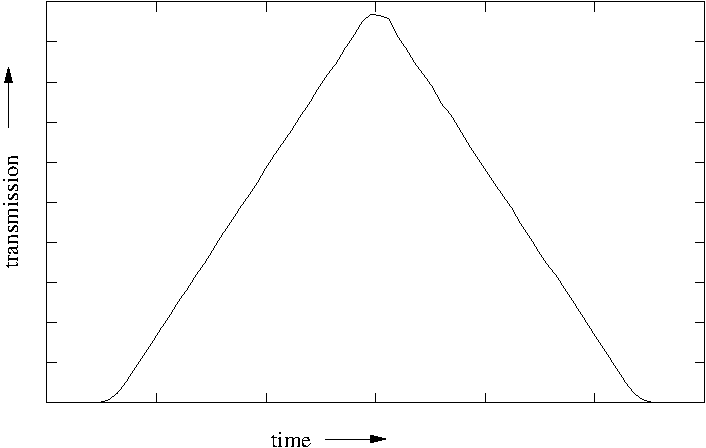
\includegraphics[width=1.0\linewidth]{figures/tracho.eps}
\caption{example transmission curve for the disc chopper\label{f:chopper2}}
\end{figure}

When simulating the chopping of a continuous beam,
most of the neutrons could easily be lost.
To improve efficiency, one can set the flag \verb+IsFirst+, which will
allow every neutron ray to pass the {\bf Chopper}, but modify the
time, $t$, to a time at which it is possible to pass.
This can also be used with TOF-instruments, which often
define the starting time of the neutrons at
the position of the first chopper.
Of course, there should be only one ``first chopper'' in
any simulation.
To simulate frame overlap from a ``first chopper'', one can specify
the number of frames to study by the parameter $n_{\rm pulse}$.

%\newpage
%\input{chopper_fermi}

\newpage
\section{V\_selector: A rotating velocity selector}
\label{vselector}
\index{Optics!Velocity selector}

\component{V\_selector}{System}{$L_0$, $L_1$, $\omega$, $r_0$, $\phi$, $N$}{}{validated, position is center of input aperture}

\begin{figure}
  \begin{center}
    \includegraphics[width=0.9\textwidth]{figures/vselector.eps}
  \end{center}
\caption{A velocity selector}
\label{f:vselector}
\end{figure}

The component {\bf V\_selector} models a rotating velocity
selector constructed from a number of collimator blades
arranged radially on an axis. Two identical slits
at a 12 o'clock position allow
neutron passage at the position of the blades.
The blades are "twisted" on the axis so that a stationary
velocity selector does not transmit any neutrons; the total
twist angle is denoted $\phi$.
By rotating the selector you allow
transmittance of neutrons around certain velocities, given by
\begin{equation}
V_0 = \omega L / \phi ,
\end{equation}
which means that the selector has turned the twist angle
$\phi$ during the neutron flight time $L/V_0$.

Neutrons having a velocity slightly smaller or larger than $V_0$
will either be transmitted or absorbed depending on the exact position
of the rotator blades when the neutron enters the selector.
Assuming this position to be unknown (and assuming infinitely
thin blades), we arrive at
\begin{equation}
T = \left\{
 \begin{array}{ll}
 1 - (N/2\pi ) |\phi-\omega L / V| &
        {\rm if}\,  -1 < (N/2\pi )(\phi -\omega L / V) < 1 \\
    0  &  {\rm otherwise}
 \end{array} \right.
\end{equation}
where $N$ is the number of collimator blades.

A horisontal divergence changes the above formula because of the
angular difference between the entry and exit points of the neutron.
The resulting transmittance resembles the one above, only with
$V$ replaced by $V_z$ and $\phi$ replaced by $(\phi +\psi )$,
where $\psi$ is the angular difference due to
the divergence. An additional vertical divergence does not change
this formula, but it may contribute to $\psi$.
(We have here ignored the very small non-linearity of $\psi$ along the
neutron path in case of both vertical and horisontal divergence).

Adding the effect of a finite blade thickness, $t$, reduces the transmission
by the overall amount
\begin{equation}
dT = (N t) / (2\pi r ) ,
\end{equation}
where $r$ is the distance from the rotation axis. We ignore the variation
of $r$ along the neutron path and use just the average value.

The input parameters for V\_selector are the slit dimensions,
\textit{width}, \textit{height} (in m),
the distance between apertures, $L_0$ (in m), the length of the
collimator blades, $L_1$ (in m), the height from rotation axix to the slit
centre, $r_0$ (in m), the rotation speed $\omega$ (in rpm)
the twist angle $\phi$ (in degrees), the blade thickness $t$ (in m),
and the number of blades, $N$.

The local coordinate system is centered at the slit centre.
The component Selector produces equivalent results.



\newpage
% Emacs settings: -*-mode: latex; TeX-master: "manual.tex"; -*-

\chapter{Monochromators}

In this class of components, we are concerned with elastic Bragg
scattering from monochromators. {\bf Monochromator\_flat} 
models a flat thin mosaic crystal with a single scattering vector
perpendicular to the surface.  
The component {\bf Monochromator\_curved} is physically similar, 
but models a singly or doubly bend monochromator crystal arrangement.

A much more general model of scattering from a single crystal is 
found in the component {\bf Single\_crystal},
which is presented under Samples, chapter~\ref{c:samples}.

% Emacs settings: -*-mode: latex; TeX-master: "manual.tex"; -*-

\section{Monochromator\_flat: An infinitely thin, flat mosaic crystal with
a single scattering vector}
\label{s:monochromator_flat}

\component{Monochromator\_flat}{System}{$z_{\rm min}$, $z_{\rm max}$, $y_{\rm min}$, $y_{\rm max}$, $\eta_{\rm h}$, $\eta_{\rm v}$, $r_0$, $Q$}{$d_{\rm m}$}{}


This component simulates an infinitely thin single
crystal with a single scattering vector perpendicular to the
surface and a mosaic spread. A typical
use for this component is to simulate a simple monochromator or analyzer.

The physical model used in the component is a rectangular piece of
material composed of a large number of small micro-crystals.
The orientation of the
micro-crystals deviates from the nominal crystal orientation so that the
probability of a given micro-crystal orientation is proportional to a
Gaussian in the angle between the given and the nominal orientation. The
width of the Gaussian is given by the mosaic spread, $\eta$, of the crystal.
$\eta$ is assumed to be large compared to the inherent Bragg width of the
scattering vector (often a few arc seconds).
The horizontal and vertical mosaicities, $\eta_{\rm h}$ and $\eta_{\rm v}$,
respectively, are allowed to be different.

The monochromator dimensions are given by the length, $z_{\rm w}$, and
the height, $y_{\rm h}$. As the parameter names indicate, the
monochromator is initially placed in the $z-y$ plane. This definition
is made to ensure that the physical monochromator angle \verb+A1+
will equal the \MCS rotation angle around the $y$-axis.

As a further simplification, the crystal is assumed to be infinitely
thin. This means that multiple scattering effects are not simulated. It
also means that the total reflectivity is used as a parameter for
the model rather than the atomic scattering cross section, implying that
the scattering efficiency does not vary with neutron wavelength.
The variance
of the lattice spacing ($\Delta d/d$) is assumed to be zero, so this
component is not suitable for simulating backscattering instruments (use
the component {\rm Single\_crystal}
in section~\ref{s:Single_crystal} for that).

When a neutron trajectory intersects the crystal, the first step in the
computation is to determine the probability of scattering. This
probability is then used in a Monte Carlo choice deciding whether to
scatter or transmit the neutron. The scattering probability is the sum
of the probabilities of first-order scattering, second-order, \ldots, up
to the highest order that permits Bragg scattering at the given neutron
wave length. However, in most cases at most one order will have a
significant scattering probability, and the computation thus considers
only the order that best matches the neutron wavelength. Bragg's law is
%
$$ n{\bf Q}_0 = 2{\bf k}_i\sin\theta $$
%
Thus, the scattering order is obtained simply as the integer multiple
$n$ of the nominal scattering vector ${\bf Q}_0$ which is closest to the
projection of $2{\bf k}_i$ onto ${\bf Q}_0$ (see
figure~\ref{f:mosaic_order}).
%  k=2PI/lambda
%  q=2k sin(theta)
%
%  2 PI n/k = d q/2k
%  q = n 4 PI/d
%
%  n 2PI/k = n 4 PI/q \sin\theta
%  1/k = 2/q\sin\theta
%  n q = 2k\sin\theta
\begin{figure}
  \begin{center}
    \psfrag{theta}[l][l]{$\theta$}
    \psfrag{ki}[r][r]{$2{\bf k}_{\rm i}$}
    \psfrag{Q0}[l][l]{${\bf Q}_0$}
    \psfrag{2Q0}[l][l]{$2{\bf Q}_0$}
    \psfrag{3Q0}[l][l]{$3{\bf Q}_0$}
    \psfrag{4Q0}[l][l]{$4{\bf Q}_0$}
    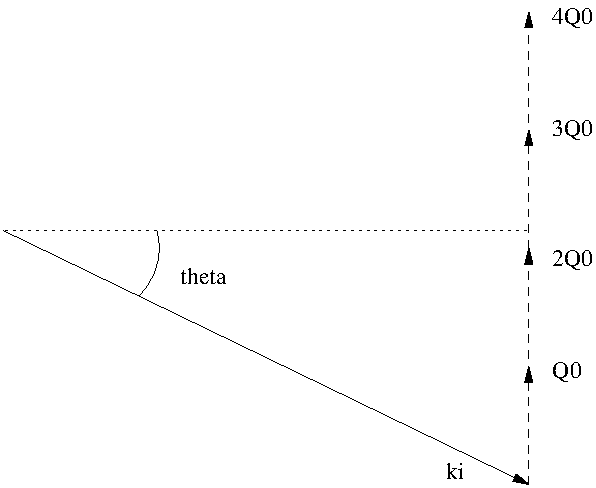
\includegraphics[width=0.5\textwidth]{figures/mosaic_order.eps}
  \end{center}
\caption{Selection of the Bragg order (``2'' in this case).}
\label{f:mosaic_order}
\end{figure}
%
Once $n$ has been determined, the Bragg angle $\theta$ can be
computed. The angle $d$ that the nominal scattering vector ${\bf Q}_0$
makes with the closest scattering vector ${\bf q}$ that admits Bragg
scattering is then used to compute the probability of reflection from
the mosaic
$$ p_{\rm reflect} = R_0 e^{-d^2/2\sigma^2}, $$
where $R_0$ is the reflectivity at the Bragg angle (see
figure~\ref{f:mosaic_angle}). The probability $p_{\rm reflect}$ is used
in a Monte Carlo choice to decide whether the neutron is transmitted or
reflected.
%
\begin{figure}
  \begin{center}
    \psfrag{th}[r][r]{$\theta$}
    \psfrag{ki}[r][r]{$2{\bf k}_{\rm i}$}
    \psfrag{kf}[l][l]{$2{\bf k}_{\rm f}$}
    \psfrag{Q0}[l][l]{${\bf Q}_0$}
    \psfrag{d}[c][c]{$d$}
    \psfrag{q}[l][l]{$\bf q$}
    \includegraphics[width=0.5\textwidth]{figures/mosaic_angle.eps}
  \end{center}
\caption{Computing the deviation $d$ from the nominal scattering direction.}
\label{f:mosaic_angle}
\end{figure}

In the case of reflection, the neutron will be scattered into the
Debye-Scherrer cone, with the probability of each point on the cone
being determined by the mosaic. The Debye-Scherrer cone can be described
by the equation
\begin{equation}
  \label{eq:mosaic_cone}
  {\bf k}_{\rm f} = {\bf k}_{\rm i}\cos2\theta +
      \sin2\theta({\bf c}\cos\varphi + {\bf b}\sin\varphi),
      \qquad\varphi\in[-\pi;\pi],
\end{equation}
where ${\bf b}$ is a vector perpendicular to ${\bf k}_{\rm i}$ and ${\bf
Q}_0$, ${\bf c}$ is perpendicular to ${\bf k}_{\rm i}$ and ${\bf b}$,
and both ${\bf b}$ and ${\bf c}$ have the same length as ${\bf k}_{\rm
  i}$ (see figure~\ref{f:mosaic_cone}). When choosing $\varphi$ (and
thereby ${\bf k}_{\rm f}$), only a small part of the full $[-\pi; \pi]$
range will have appreciable scattering probability in non-backscattering
configurations. The best statistics is thus obtained by sampling
$\varphi$ only from a suitably narrow range.

The (small) deviation angle $\sigma$ of ${\bf q}$ from the nominal
scattering vector $n{\bf Q}_0$ corresponds to a $\Delta q$ of
$$ \Delta q \approx \sigma 2k\sin\theta. $$
The angle $\varphi$ corresponds to a $\Delta k_{\rm f}$ (and hence
$\Delta q$) of
$$ \Delta q \approx \varphi k \sin(2\theta) $$
(see figure~\ref{f:mosaic_cone}).
Hence we may sample $\varphi$ from a Gaussian with standard deviation
$$ \sigma\frac{2k\sin\theta}{k\sin(2\theta)} =
\sigma\frac{2k\sin\theta}{2k\sin\theta\cos\theta} =
\frac{\sigma}{\cos\theta} $$
to get good statistics.
%
\begin{figure}
  \begin{center}
    \psfrag{th}[r][r]{$2\theta$}
    \psfrag{ki}[c][c]{$2{\bf k}_{\rm i}$}
    \psfrag{kf}[r][r]{$2{\bf k}_{\rm f}$}
    \psfrag{nQ0}[l][l]{$n{\bf Q}_0$}
    \psfrag{q}[l][l]{$\bf q$}
    \psfrag{2ksin2t}[l][l]{$2 k \sin(2 \theta)$}
    \includegraphics[width=0.5\textwidth]{figures/mosaic_cone.eps}
  \end{center}
\caption{Scattering into the part of the Debye-Scherrer cone covered by
    the mosaic.}
\label{f:mosaic_cone}
\end{figure}

What remains is to determine the neutron weight. The distribution from
which the scattering event is sampled is a Gaussian in $\varphi$ of
width $\frac{\sigma}{\cos\theta}$,
$$ f_{\rm MC}(\varphi) = \frac{1}{\sqrt{2\pi}(\sigma/\cos\theta)}
            e^{-\varphi^2/2(\sigma/\cos\theta)^2}
$$
In the physical model, the probability of the scattering event is
proportional to a Gaussian in the angle between the nominal scattering
vector ${\bf Q}_0$ and the actual scattering vector ${\bf q}$. The
normalization condition is that the integral over all $\varphi$ should
be 1. Thus the probability of the scattering event in the physical model
is
\begin{equation}
  \label{eq:mosaic_integral}
  \Pi(\varphi) = e^{\frac{-d(\varphi)^2}{2\sigma^2}} /
   \int_{-\pi}^{\pi} e^{\frac{-d(\varphi)^2}{2\sigma^2}} d\varphi
\end{equation}
where $d(\varphi)$ denotes the angle between the nominal scattering
vector and the actual scattering vector corresponding to $\varphi$.
According to equation~(\ref{probrule}), the weight adjustment $\pi_j$ is
then given by
$$ \pi_j = \Pi(\varphi) / f_{\rm MC}(\varphi). $$
In the implementation, the integral in~(\ref{eq:mosaic_integral}) is computed
using a 15-order Gaussian quadrature formula, with the integral
restricted to an interval of width $5\sigma/\cos\theta$ for the same
reasons discussed above on the sampling of $\varphi$.

The input parameters for Mosaic\_simple are \textit{zmin},
\textit{zmax}, \textit{ymin}, and \textit{ymax} to define the surface of
the crystal in the Y-Z plane; \textit{mosaic} to give the FWHM of the
mosaic spread; \textit{R0} to give the reflectivity at the Bragg angle,
and \textit{Qx}, \textit{Qy}, and \textit{Qz} to give the scattering
vector.


\newpage
% Emacs settings: -*-mode: latex; TeX-master: "manual.tex"; -*-

\section{Monochromator\_curved: An infinitely thin, curved mosaic crystal with
a single scattering vector}
\label{s:monochromator_curved}

\component{Monochromator\_curved}{System, Peter Link}{$z_{\rm w}$, $y_{\rm h}$, gap, $\eta_{\rm h}$, $\eta_{\rm v}$, $n_{\rm h}$, $n_{\rm v}$, $R_0$, $Q$, $r_{\rm h}$, $r_{\rm v}$}{$d_{\rm m}$, $\eta$, $h$, $w$, verbose, transmit, reflect}{}

\begin{figure}
  \begin{center}
    \includegraphics[width=0.9\textwidth]{figures/monochromator_curved.eps}
  \end{center}
\caption{A curved monochromator}
\label{f:monochromator_curved}
\end{figure}


This component simulates an array of infinitely thin single
crystals with a single scattering vector perpendicular to the
surface and a mosaic spread.
This component is used to simulate a singly or doubly
curved monochromator or analyzer, in reflecting geometry.

The component uses  rectangular pieces of monochromator material
as described in {\bf Monochromator\_curved}.
The important parameters are the piece height and width,
$y_{\rm h}$ and $z_{\rm w}$, respectively, the
horizontal and vertical mosaicities, $\eta_{\rm h}$ and $\eta_{\rm v}$,
respectively. The number of pieces vertically and horizontally are called
$n_{\rm v}$ and $n_{\rm h}$, respectively, and the vertical and horizontal
radii of curvature are named $r_{\rm v}$ and $r_{\rm h}$, respectively.
The scattering vector is named $Q$, and as described in
{\bf Monochromator\_flat}, multiples of $Q$ can be applied.
All single crystals are positioned in the same vertical plane, but tilted accordingly to the curvature radius.

If just one mosaicity, $\eta$, is specified, this the same for
both directions.

The constant monochromator reflectivity, $R_0$ can be replaced by
a file of tabulated reflectivities. In the same sense, the transmission
can be modeled by a tabulated file (for non reflected neutrons).

As for {\bf Monochromator\_flat}, the crystal is assumed to be infinitely
thin, and the varition in lattice spacing, ($\Delta d/d$),
is assumed to be zero. Hence, this
component is not suitable for simulating backscattering instruments or to
investigate multiple scattering effects.

The algorithm for scattering and calculation of the neutron weight for
the individual blades is described under {\bf Monochromator\_flat}.



% Emacs settings: -*-mode: latex; TeX-master: "manual.tex"; -*-

\chapter{Samples}
\index{Library!Components!samples}

This class of components models the sample of the experiment.
This is by far the most challenging part of a neutron scattering
instrument to model. However, for purpose of simulating
instrument performance, details of the samples are rather unimportant,
allowing for simple approximations. On the contrary, for full
virtual experiments it is of importance to have realistic and
detailed sample descriptions. \MCS\ contains both simple and detailed
samples, although there is still room for much more development.

We first consider incoherent scattering. The simple component {\bf Vanadium}
performs both incoherent scattering and absorption.

An important component class is elastic Bragg scattering from an ideal powder.
The components {\bf Powder1} and {\bf Powder2} model a simple powder with one or two
reflections and incoherent scattering. Finally, the {\bf PowderN} component extends the capabilities to N lines, read from a LAZY/Crystallographica data file.

Next type is Bragg scattering from single crystals.
The simplest single crystals are in fact the monochromator components
{\bf Monochromator\_flat} and {\bf Monochromator\_curved},
which were presented in the section on optics.
The monochromators are models of a thin mosaic crystal
with a single scattering vector perpendicular to the surface.
Much more advanced, the component {\bf Single\_crystal}
is a general single crystal sample (with multiple scattering) that allows
the input of an arbitrary unit cell and a list of structure factors, and
also allows anisotropic mosaic and $\Delta d/d$ lattice space variation.

Isotropoic small-angle scattering is simulated in {\bf Sans\_Spheres},
which models scattering from a collection of hard spheres. A more general
SANS sample is highly wanted. In addition, a reflectometry sample
should be developed.

Inelastic scattering from a dispersion is exemplified by
the relatively simple component {\bf Phonon}.

For a more general sample model, the {\bf Isotropic\_Sqw} component is able to simulate all kinds of isotropic materials: liquids, glasses, polymers, powders, ... Physical processes include coherent/incoherent scattering, both elastic and inelastic, with absorption and multiple scattering. Moreover, this compoennt may be used concentrically, to model a sample environment. Thus it may handle most samples except single crystals.

In general, all samples are assumed to be homogeneous. There would also be
potential in developing an inhomogeneous sample, e.g. with
spatially varying lattice constant, relevant for stress/strain scanners.
Inhomogeneously absorbing sample for tomography could also be possible.
Further, no polarization effects are yet taken into account in any
of the samples.

\begin{table}
  \begin{center}
  {\let\my=\\
    \begin{tabular}{|c|cc|cc|c|c|}
    \hline
    Sample        & \multicolumn{2}{c|}{Coherent} & \multicolumn{2}{c|}{Incoherent} &&\\
    Process       & Elastic & Inelastic & Elastic & Inelastic & Absorption & Multi. Scatt.\\
    \hline
    Phonon\_simple&         & X         &         &           & X & \\
    Isotropic\_Sqw&  X      & X         & X       & X         & X & X \\
    Powder1       &  1 line &           &         &           & X & \\
    PowderN       &  N lines&           &         &           & X & \\
    Sans\_spheres &  colloid&           &         &           & X & \\
    Single\_crystal& X      &           & X       &           & X & X \\
    V\_sample     &         &           & X       &           & X & \\
    \hline
    \end{tabular}
    \caption{Processes implemented in sample components}
    \label{t:sample-process}
  }
  \end{center}
\end{table}

\input{vanadium.tex}
\input{powder2.tex}
\input{Single_crystal.tex}
\section{Sans\_spheres: A sample of hard spheres for small-angle scattering}
\label{sans}
\index{Samples!Dilute colloid medium}
\index{Diffraction}
\index{Small angle scattering}

\component{Sans\_spheres}{(System); Lise Arleth, Veterinary University of Denmark}{$R$, $x_w$, $y_h$, $z_t$, $r$, $\sigma_a$}{$phi$, $q_{max}$, $\Delta \rho$}{}

The component {\bf Sans\_spheres} models a sample of small independent
spheres of radius $R$, which are uniformly distributed
in a rectangular volume $x_w \times y_h \times z_t$ with a volume
fraction $\phi$. The absorption cross section density for the spheres
(or is it from the solution?)
is $\sigma_a$ (in units of m$^{-1}$), specified
for neutrons at 2200 m/s. Absorption and incoherent scattering from the medium
is neglected.
The difference in scattering length density
(the contrast) between the hard spheres and the medium is called $\Delta \rho$.
$q_{\rm max}$ denotes the maximum scattered $q$-value that is probed
in the simulation.

\subsection{Small-angle scattering cross section}
The neutron intensity scattered in a solid angle $\Delta \Omega$
for a flat transmission isotropic SANS sample is given by \cite{ILLblue}:
\begin{equation}
I_s(q) = \Psi \Delta\Omega T A z_{\rm max} \frac{d\sigma_v}{d\Omega}(q) ,
\end{equation}
where $\Psi$ is the neutron flux, $T$ is the sample transmission,
$A$ is the illuminated sample area, and $z_{\rm max}$ the length of
the neutron path through the sample.

In this component, we consider only scattering from a thin solution
of monodisperse hard spheres of radius $R$, where the volume-specific
scattering cross section is given by \cite{ILLblue}
\begin{equation}
\frac{d\sigma_v}{d\Omega}(q) =
  n (\Delta\rho)^2 V^2 \left( 3\frac{\sin(qR)-qR\cos(qR)}{(qR)^3} \right)^2 .
\end{equation}
Here, $n$ is the number density of spheres, and $V$ is the
sphere volume. Their product gives the input parameter, $\phi=nV$.

\subsection{Algorithm}
All neutrons, which hit the sample volume, are scattered.
(Hence, no direct beam is simulated.)
For scattred neutrons, the following steps are taken:
\begin{enumerate}
\item Choose a value of $q$ uniformly in the interval $[0;q_{\rm max}]$.
\item Choose a polar angle, $\alpha$,
  for the {\bf q}-vector uniformly in $[0;\pi]$.
\item Scatter the neutron according to $(q,\alpha)$.
\item Calculate and apply the correct weight factor correction.
\end{enumerate}

% Emacs settings: -*-mode: latex; TeX-master: "manual.tex"; -*-


\section{Phonon\_simple: A simple phonon sample}
\label{s:phonon_simple}
\index{Samples!Isotropic acoustic phonon}
\index{Inelastic scattering}

\component{Phonon\_simple}{Kim Lefmann}{ $r_{\rm o}$, $h$, $r_{\rm foc}$, $x_{\rm target}$, $y_{\rm target}$, $z_{\rm target}$, $\sigma_{\rm abs}$, $\sigma_{\rm inc}$, $a$, $b$, $M$, $c$, $DW$, $T$}{$w_x$, $h_y$, $t_z$, $w_{\rm focus}, h_{\rm focus}$, $w_{\rm foc, angle}$, $h_{\rm foc, angle}$, target\_index}{}
This component models a simple phonon signal from a single crystal of 
one element in an {\em fcc} crystal structure.
Only one isotropic acoustic phonon branch is modeled, and the longitudinal
and transverse dispersions are identical with the velocity of sound being $c$.
Other physical parameters are the atomic mass, $M$, the lattice parameter, $a$,
the scattering length, $b$,
the Debye-Waller factor, \verb+DW+, and the temperature, $T$.

Incoherent scattering and absorption are also taken into account by the cross
sections $\sigma_{\rm abs}$ and $\sigma_{\rm inc}$.

The sample can have the form of a cylinder with height $h$ and radius
$r_0$, or a box with dimensions $w_x, h_y, t_z$. 

Phonons are emitted into a specific range of solid angles, specified 
by the location $(x_t, y_t, z_t)$ and the focusing radius, $r_0$.
Alternatively, the focusing is given by a rectangle, 
$w_{\rm focus}$ and $h_{\rm focus}$, and the focus point is given by the
indeox of a down-stream optical element, \verb+target_index+.

Multiple scattering is not included in this component. The scattering
cross section is given by the detailed calculations below.

\subsubsection{The phonon cross section} % This is taken directly from the paper %
The inelastic phonon cross section for a Bravais crystal of a pure element
is given by Ref.~\cite[ch.3~]{squires} 
\begin{eqnarray}
\frac{d^2\sigma'}{d\Omega dE_{\rm f}} &=&
  b^2 \frac{k_{\rm f}}{k_{\rm i}} \frac{(2\pi)^3}{V_0}\frac{1}{2M} \exp(-2W) \nonumber \\
&\times&
  \sum_{\tau,q,p} \frac{(\mbox{\boldmath $\kappa$} \cdot {\bf e}_{q,p})^2}
                       {\omega_{q,p}} 
  \left\langle n_{q,p} + \frac{1}{2} \mp \frac{1}{2} \right\rangle
  \delta(\omega\pm\omega_{q,p}) \delta(\kappa\pm{\bf q}-\tau) ,
\end{eqnarray}
where both annihilation and creation of one phonon is considered
(represented by the plus and minus sign in the dispersion relation,
respectively).
In the equation, 
$\exp(-2W)$ is the Debye-Waller factor, \verb+DW+ and
$V_{\rm c} = \rho_{\rm c}^{-1}$ is the volume of the unit cell.
The sum runs over the reciprocal lattice vectors, $\tau$, 
over the polarisation index, $p$,
and the $N$ allowed wave vectors {\bf q} within the Brillouin zone
(where $N$ is the number of unit cells in the crystal).
Further, ${\bf e}_{q,p}$ is the
polarization unit vectors, $\omega_{q,p}$ the phonon dispersion,
and $\langle n_{q,p} \rangle$ is the Bose factor at the given value of
$\hbar |\omega_{q,p}|/(k_{\rm B}T)$.

We have simplified this expression by assuming no polarization
dependence of the dispersion, giving 
$\sum_{p} (\mbox{\boldmath $\kappa$} \cdot {\bf e}_{q,p})^2 = \kappa^2$.
We assume that the inter-atomic interaction is nearest-neighbour-only
so that the phonon dispersion becomes: 
\begin{equation}
d_1({\bf q}) = c_1/a \sqrt(z-s_q) ,
\end{equation}
where $z=12$ is the number of nearest neighbours and 
$s_q=\sum_{\rm nn} \cos({\bf q} \cdot {\bf r}_{\rm nn})$,
where in turn ${\bf r}_{\rm nn}$ is the lattice positions of the 
nearest neighbours.

This dispersion relation may be modified with a small effort,
since it is given as a separate c-function attatched to the component.

To calculate $d\sigma/d\Omega$ we need to transform the 
{\bf q} sum into an integral over the Brillouin zone by 
$\sum_q \rightarrow N V_{\rm c} (2\pi)^{-3} \int_{\rm BZ} d^3{\bf q}$.
The $\mbox{\boldmath $\kappa$}$ sum can now be removed by
expanding the {\bf q} integral to infinity. 
All in all, the partial differential cross section reads
\begin{eqnarray}
\frac{d^2\sigma'}{d\Omega dE_{\rm f}}
  (\mbox{\boldmath $\kappa$},\omega) &=&
  b^2 \frac{k_{\rm f}}{k_{\rm i}} N \frac{1}{2M} 
  \int \frac{\hbar \kappa^2}{c_1 |{\bf q}-{\bf Q}|} 
  \left\langle n_{q}+\frac{1}{2}\mp\frac{1}{2} \right\rangle
  \delta(\omega\pm\omega_{q}) \delta(\mbox{\boldmath $\kappa$}\pm{\bf q}) 
   d^3{\bf q} \nonumber \\
 &=& b^2 \frac{k_{\rm f}}{k_{\rm i}} N 
          \frac{\hbar^2 \kappa^2}{2M c_1|{\bf q}-{\bf Q}|} 
  \left\langle n_{\kappa}+\frac12\pm\frac12 \right\rangle 
  \delta(\hbar\omega\pm d_1(\kappa)) .
\end{eqnarray}
Using the integration sketched in eq.~(\ref{eq:dcsdisp}), we reach
*** CHECK THIS!! ***
\begin{equation} \label{eq:phononcross}
\left(\frac{d\sigma'}{d\Omega}\right)_j =
b^2 \frac{k_{\rm f}^2}{k_{\rm i}} N 
\frac{\hbar^4 \kappa^2}{2Mm c_1 |{\bf q}-{\bf Q}| J(k_{{\rm f},j})} 
\left\langle n_{\kappa}+\frac12\pm\frac12 \right\rangle . 
\end{equation}
A rough order-of-magnitude consideration gives
$\frac{\hbar^2 k_{{\rm f},j}}{mJ(k_{{\rm f},j})} \approx 1$,
$\frac{k_{{\rm f},j}}{k_{{\rm f},i}}\approx 1$,
$\langle n_{\kappa}+\frac12\pm\frac12 \rangle \approx 1$,
$\frac{\hbar^2\kappa^2}{2M\hbar\omega_\kappa}
\approx \frac{m}{M}$ (for large disperison values?????).
Hence, $\left(\frac{d\sigma}{d\Omega}\right)_j \approx N b^2 \frac{m}{M}$, and
$\sigma_{\rm inel}$ becomes a fraction of $4 \pi N b^2$, as one
would expect.
The differential cross section per unit cell is found from 
(\ref{eq:phononcross}) by letting $N=1$. 

\subsubsection{The algorithm}
(*** SEE IF THIS IS WRITTEN ELSEWHERE ***)

\subsubsection{The weight transformation}
The total weight transformation becomes
\begin{equation} \label{eq:phonon_mult}
\pi_i = a_{\rm lin} \rho_c l_{\rm max} n_{\rm s} \Delta \Omega
 b^2 \frac{k_{\rm f}^2}{k_{\rm i}}
 \frac{\hbar^4 \kappa}{2Mm c_1 |{\bf q}-{\bf Q}| J(k_{{\rm f},j})} 
 \left\langle n_{\kappa}+\frac12\pm\frac12 \right\rangle ,
\end{equation}
where the Jacobian reads
\begin{equation}
J = -\frac{\hbar^2}{m} k_{\rm f} 
    - c \frac{\partial}{\partial k_{\rm f}} 
        \left| {\bf k}_{\rm i} - k_{\rm f} \hat{k}_{\rm f} \right| .
\end{equation}



\section{Isotropic\_Sqw: A general $S(q,\omega)$ coherent and incoherent scatterer}
\label{s:isotropic-sqw}
\index{Samples!Coherent and incoherent isotropic scatterer}
\index{Coherent and incoherent isotropic scatterer}
\index{Inelastic scattering}

\component{Isotropic\_Sqw}{V. Hugouvieux, E. Farhi}{Sqw$\_{coh}$, $\sigma_{coh}$, Sqw$\_{inc}$, $\sigma_{inc}, V_\rho, \sigma_{abs}, T$}{$q_{min}, q_{max}, \omega_{min}, \omega_{max}, d\phi$, order}{not fully validated}

\begin{figure}
  \begin{center}
    \includegraphics[width=0.9\textwidth]{figures/sqw.eps}
  \end{center}
\caption{An $l-^4$He sample in a cryostat, simulated with the Isotropic\_Sqw component in concentric geometry.}
\label{f:isotropic-sqw}
\end{figure}

The component assumes that the sample has the structure of a liquid. This stands for indeed normal liquids, glasses (amorphous systems), polymers, and may be extended to powders.

\subsection{A short introduction to the theory of liquids}

\begin{figure}
  \begin{center}
    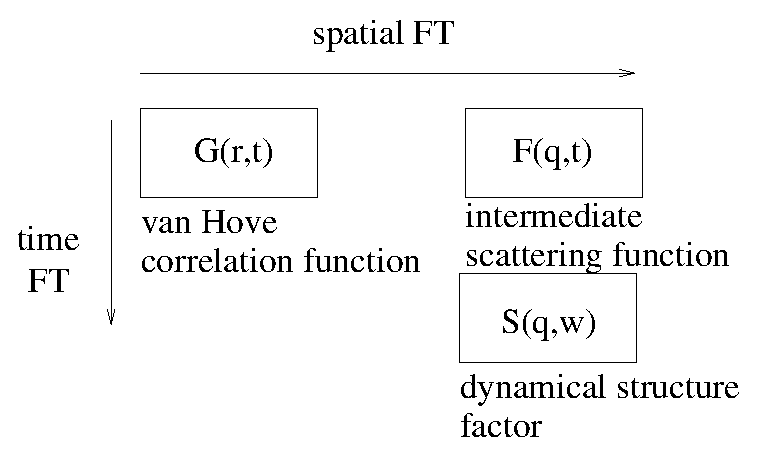
\includegraphics[width=0.9\textwidth]{figures/GFS.eps}
  \end{center}
\caption{Relations between dynamical functions using space, time, wavevector and energy variables.}
\label{f:GFS}
\end{figure}

In the case of a homogeneous and classical liquid, the \emph{van Hove correlation function}, which describes the time and space correlations in the liquid, can be written \cite{Egelstaff67,squires}:
\begin{equation} \label{eq:vanhove}
G(\vec{r},t) = \frac{1}{N} \sum_{i=1}^N \sum_{j=1}^N  \langle\delta[\vec{r} + \vec{r}_i(0) - \vec{r}_j(t)]\rangle
\end{equation}
with $\vec(r)$ and $t$ being the position and time of the atom distribution in the liquid.
Using the particule-density function $\rho(\vec(r),t)$, the function $G$ can be rewritten:
\begin{equation} \label{eq:vanhove-rho}
G(\vec{r},t) = \frac{\langle \rho(0,0) \rho(\vec{r},t)\rangle}{\rho}
\end{equation}

On the experimental point of view, one usually refers to the \emph{dynamical structure factor} $S(q,\omega)$, which is the double Fourier-transform in space and time of the van Hove correlation function $G(r,t)$:
\begin{eqnarray} \label{eq:sqw-rho}
S(q,\omega) &= \frac{1}{2\pi}\int_{-\infty}^{\infty} F(\vec{q},t) e^{-i\omega t} dt \nonumber \\
            &= \frac{1}{2\pi N} \int_{-\infty}^{\infty} \langle \hat\rho^*(\vec{q},0) \hat\rho(\vec{q},t) \rangle e^{-i\omega t} dt.
\end{eqnarray}
where $\hat\rho(\vec{q}, t)$ is the spatial Fourier transform of the density $\rho(\vec{r},t)$, and the \emph{intermediate scattering function} $F$ is the time correlation function of $\hat\rho$:
\begin{eqnarray}
F(\vec{q},t) &= \frac{1}{N} \langle \hat\rho^*(\vec{q},0)  \hat\rho(\vec{q},t) \rangle \nonumber \\
                    &= \frac{1}{N} \sum_{i=1}^N \sum_{j=1}^N \langle e^{i \vec{q}.(\vec{r}_j(t) - \vec{r}_i(0))} \rangle
\end{eqnarray}
Some easely measureable quantities in a liquid are the \emph{pair correlation function} $g(r)$ and the \emph{structure factor} $S(q)$, defined as:
\begin{eqnarray}
\rho g(\vec{r}) &= \frac{1}{N} \sum_{i=1}^N \sum_{j \neq i} \langle \delta(\vec{r}+\vec{r}_i-\vec{r}_j) \rangle \\
S(\vec{q}) &=1 + \rho \int_V [g(\vec{r})-1] e^{i\vec{q}.\vec{r}} d\vec{r} \\
           &=1 + \rho \int_{0}^{\infty} [g(r)-1] \frac{\sin(qr)}{qr} 4 \pi r^2 dr {\rm in isotropic materials}
\end{eqnarray}
Both $g(r)$ and $S(q)$ converge to unity for large $r$ and $q$ values respectively, and they are representative of the atoms spatial distribution.


Following Squires (\cite{squires}, p63), the neutron differential scattering cross section for both coherent and incoherent processes is
\begin{equation}
\frac{d^2\sigma}{d\Omega dE_f} = \frac{\sigma}{4\pi}\frac{k_f}{k_i} N S(q, \omega)
\end{equation}
with usual notations. The unit of the dynamical structure factor $S$ is an inverse energy.

\subsection{How does a neutron interact with the material ?}


\subsection{The implementation}
\subsubsection{Choosing the interaction position}
\subsubsection{Choosing the type of interaction}
\subsubsection{Choosing the $q$ and $\omega$ transfert}
%\input{LSCO.tex}


% Emacs settings: -*-mode: latex; TeX-master: "manual.tex"; -*-

\chapter{Monitors and detectors}

In real neutron experiments, detectors and monitors play quite
different roles. One wants the detectors to be as efficient as 
possible, counting all neutrons (absorbing them in the process), 
while the monitors measure the intensity of the incoming beam, and must
as such be almost transparent, interacting only with (roughly) 0.1-1\%
of the neutrons passing by. In computer simulations, it is 
of course possible to detect every neutron without 
absorbing it or disturbing any of its parameters. Hence, the two components
have very similar functions in the simulations, and we do
not distinguish between them. For simplicity, they are from here on
just called monitors, since they do not absorb neutrons.

Another important difference between computer simulations 
and real experiments is
that one may allow the monitor to be sensitive to any neutron property,
as {\em e.g.} direction, energy, and divergence, in addition to what
is found in advanced existing monitors (space and time). One may, in
fact, let the monitor have several of these properties at the same time,
as seen for example in the energy sensitive monitor in
section~\ref{s:e_monitor}.

When a monitor detects a neutron ray, 
a number counting variable is incremented: $n_i = n_{i-1}+1$
In addition, the neutron
weight $p_i$ is added to the weight counting variable:
$I_i = I_{i-1} + p_i$, 
and the second moment of the weight is
updated: $M_{2,i} = M_{2,i-1} + p_i^2$. 
As also discussed in the System Manual, after a simulation of $N$ rays
the detected intensity (in units of neutrons/sec.) is $I_N$,
while the estimated errorbar is $\sqrt{M_{2,i}^2}$.


Many different monitor components have been developed for
\MCS , but we have selected to support only the most important ones.
One example of the monitors we have omitted is the single monitor,
{\bf Monitor},
that measures just one number (with errorbars) per simulation.
This effect is mirrored by any of the 1- or 2-dimensional detectors
we support, e.g. the {\rm PSD\_monitor}. 
In case additional functionality of monitors is required,
the existing monitors can easily be modified.
However, the ultimate solution is the use of the 
``Swiss army knife'' of monitors, {\rm Monitor\_nD}, that can face
almost any simulation challenge. 

\newpage
% Emacs settings: -*-mode: latex; TeX-master: "manual.tex"; -*-

\section{TOF\_monitor: The time-of-flight monitor}
\component{TOF\_monitor}{System}{$x_{\rm min}$, $x_{\rm max}$, $y_{\rm min}$, $y_{\rm max}$, $n_{\rm chan}$, $t_0$, $t_1$, filename}{$\Delta t$}

The component {\bf TOF\_monitor} has a rectangular opening
in the $x-y$ plane, given by the $x$ and $y$ parameters,
like for {\rm Slit}. 
The neutron is propagated to the plane of the monitor
by the kernel call PROP\_Z0.
Any neutron ray that passes within the opening is counted, and
the total neutron counts are updated:

Special about {\bf TOF\_monitor} is that it is sensitive to
the time, $t$, where the neutron ray is hits the component.
Like in a real time-of-flight detector, the time dimension is
binned into small time intervals. 
Hence this monitor updates a one-dimensional array of counts.
The $n_{\rm chan}$ time intervals begin at $t_0$ and 
end at $t_1$ (or have each length $dt$ if this parameter is specified). 
As usual in time-of-flight analysis, all times are given in units of $\mu$s.

The output parameters from {\bf TOF\_monitor} are the three count numbers, 
$N, I$, and $M_2$ for the total counts in the monitor.
In addition a file is produced with a list of the same three data divided in
different TOF bins.
This file can be read and plotted by the {\rm MCplot} tool; see the
System Manual.



\newpage
% Emacs settings: -*-mode: latex; TeX-master: "manual.tex"; -*-

\section{E\_monitor: The energy-sensitive monitor} \label{s:e-monitor}
\index{Monitors!Energy monitor}
\component{E\_monitor}{System}{$x_{\rm min}$, $x_{\rm max}$, $y_{\rm min}$, $y_{\rm max}$, $n_{\rm chan}$, $E_{\rm min}$, $E_{\rm max}$, filename}{}{}

The component {\bf E\_monitor} resembles {\bf TOF\_monitor}
to a very large extent. Only this monitor is sensitive to
the neutron energy, which in binned in \textit{nchan} bins between
$E_{\rm min}$ and $E_{\rm max}$.

The output parameters from {\bf E\_monitor} are the total counts,
and a file with 1-dimensional data vs. $E$, similar to {\bf TOF\_monitor}.




\newpage
\input{l_monitor}

\newpage
% Emacs settings: -*-mode: latex; TeX-master: "manual.tex"; -*-

\section{PSD\_monitor: The PSD monitor}
\component{PSD\_monitor}{System}{$x_{\rm min}$, $x_{\rm max}$, $y_{\rm min}$, $y_{\rm max}$, $n_x$, $n_y$, filename}{}


The component {\bf PSD\_monitor} resembles other monitors, e.g. 
{\bf E\_Monitor}, and also propagates the neutron to the detector
surface in the $(x,y)$-plane, where the detector window is set
by the $x$ and $y$ input coordinates.
The PSD monitor, though, is not sensitive to the neutron energy, but
rather its position. the rectangular monitor window is divided
into $n_x \times n_y$ pixels, each of which acts like a single
counter.

The output from {\bf PSD\_monitor} is the integrated counts, $n, I, M_2$, 
as well as 
three two-dimensional arrays of counts: $n(x,y), I(x,y), M_2(x,y)$.
The arrays are written to a file and can be read e.g. by the tool
{\bf MC\_plot}, see the system manual.

{\bf Burde man ikke kunne specificere en radius, 
og s\aa\ blev den en 2D cylinder detektor??}

\newpage
\input{div_monitor}

\newpage
\input{divpos_monitor}

%\newpage
%\input{monitor_nd}
\chapter{Special-purpose components}
\index{Library!Components!misc}

The chapter deals with components that are not easily included
in any of the other chapters because of their special nature,
but which still are considered to be of significant importance
to \MCS .

One part of these components deals with splitting simulations
into two (or more) stages. For example, a guide system is often
not changed much, and a long simulation of neutron rays
``surviving'' through the guide system could be reused
for several simulations of the instrument back-end, speeding up
the simulations by (typically) one or two orders of magnitude.
The components for doing this trick is {\bf Virtual\_input} and
{\bf Virtual\_output}, which stores and reads neutron rays, respectively.

Another pair of components performs the simulation of the instrument
resolution functions. This is {\bf Res\_sample}, that is to be
placed at the sample position, and {\bf Res\_monitor}, that should
be localized at the position of the instrument detector.

\newpage
\section{Vitual\_input: Starting the second part of a split simulation}
\label{virtual_input}

\component{Virtual\_input}{System}{filename}{buffer size, repeat count, type}

The component {\bf Virtual\_input} resumes a split simulation where the 
first part has been performed by another instrument and the neutron ray
parameters have been stored by the component {\bf Virtual\_output}.

All neutron ray parameters are read from the input file, which is by default
of ``text'' type, but can also assume the binary formats 
``float'' or ``double''. The reading of neutron rays continue until the 
specified number of rays have been simulated or 
till the file has been exhausted. If desirable, the input file
can be reused a number of times, determined by the optional parameter
``repeat count''. However, care should be taken when dealing with 
absolute intensities, which are automatically correct only
when the input file has been exhausted once.

For performance reasons, it is possible to specify the size of 
the buffer to use in reading the neutron rays from file. Default 
is to buffer the whole file, but this may be fatal for very large
input files.

\section{Vitual\_output: Saving the first part of a split simulation}
\label{virtual_output}

\component{Virtual\_output}{System}{filename}{buffer size, type}

The component {\bf Virtual\_output} stores the neutron ray parameters
from a split simulation. It is then possible to let the 
next part of the simulation be performed by another instrument,
which reads the stored neutron ray
parameters by the component {\bf Virtual\_input}.

All neutron ray parameters are saved to the output file, which is by default
of ``text'' type, but can also assume the binary formats 
``float'' or ``double''. The storing of neutron rays continue until the 
specified number of simulations have been performed.

For performance reasons, it is possible to specify the size of 
the buffer to use in writing the neutron rays to file. Default 
is to buffer the whole file, but this may be fatal for very large
simulations.


\newpage
% Emacs settings: -*-mode: latex; TeX-master: "manual.tex"; -*-

\section{Res\_sample: A uniform scatterer for resolution calculation}
\label{s:res_sample}
\index{Samples!Resolution function, sample for}

\component{Res\_sample}{System, Alan Tennant}{$r_{\rm i}$, $r_{\rm o}$, $h$, $r_{\rm focus}$, $x_{\rm target}$, $y_{\rm target}$, $z_{\rm target}$, $E_0$, $\Delta E$ }{$x_w$, $y_h$, $z_t$, $x_{\rm focus}$, $y_{\rm focus}$, $a_{\rm v, focus}$, $a_{\rm h, focus}$, target index}{}

The component \textbf{Res\_sample} models an inelastic sample that
scatters completely homogeneous in position and energy,
within specified intervals. Regardless of
the state of the incoming neutron, all directions and energies for the
scattered neutron have the same probability. This is clearly
not a physical sample! Rather, the component is meant
for computation of the resolution function, but it may also be used
for test and debugging purposes. For calculations of the resolution
function, {\bf Res\_sample} should be used
together with the \textbf{Res\_monitor} component, described in
section~\ref{s:res_monitor}.

The shape of {\rm Res\_sample} is either a hollow cylinder
or a rectangular box, as specified for {\rm Vanadium}
(see section~\ref{s:v_sample}).The hollow cylinder shape is
specified with the inner and outer radius, $r_{\rm i}$ and $r_{\rm o}$,
respectively, and the height, $h$.
If these parameters are unspecified,
the shape is instead a box of dimensions $x_w$, $y_h$, and $z_t$.
See figure~\ref{f:res_sample}.\par
%
\begin{figure}[htbp]
  \begin{center}
        \psfrag{ri}[c][c]{\textit{radius\_i}}
        \psfrag{ro}[c][c]{\textit{radius\_o}}
        \psfrag{h}[c][c]{\textit{h}}
        \psfrag{bri}[c][c]{\textit{radius\_i}}
        \psfrag{bro}[c][c]{$-\textit{radius\_o}$}
        \psfrag{bh}[c][c]{\textit{h}}
        \psfrag{X}[c][c]{\textit{X}}
        \psfrag{Y}[c][c]{\textit{Y}}
        \psfrag{Z}[c][c]{\textit{Z}}
        \includegraphics[width=0.9\textwidth]{figures/res_sample.eps}
    \caption{The two possible shapes of the \textbf{Res\_sample} component.}
    \label{f:res_sample}
  \end{center}
\end{figure}
%
The component only propagates the neutrons that are scattered; neutrons
that would pass through or miss {\bf Res\_sample} are absorbed. There is no
modeling of the cross section of the sample, secondary extinction
\textit{etc.}; the scattering probability is proportional to the neutron
flight path length inside the sample, with the constant of
proportionality arbitrarily set to $1/(2|\textit{radius\_o}|)$. The
reason for this is that the resolution
function of an instrument (although including the sample size)
is independent of any sample properties such as scattering
and absorbtion cross sections.does not depend on the scattering
cross section.

The point of scattering in the sample is chosen uniformly
along the neutron flight path inside the sample, and the scattered
neutron is given a random energy and direction. The energy is selected in
the interval $[E_0-\Delta E; E_0+\Delta E]$ which hence must be
chosen large enough to cover all interesting neutrons. Similarly, the
direction is chosen in a user-specified range,
either within a sphere of radius $r_{\rm foc}$, within a rectangular
target with measures $(x_{\rm focus}, y_{\rm focus})$
or in the specified angular range. This target is positioned at the $x_{target}$, $y_{target}$, $z_{target}$ point in space, or using the target\_index for wich e.g. 1 is the further component, -1 is the previous, etc...

A special feature, used when computing resolution functions, is that the
component stores complete information about the scattering event in the
output parameter \textit{res\_struct}. The information includes initial
and final wave vectors, the coordinates of the scattering point, and the
neutron weight after the scattering event. From this information the
scattering parameters $({\bf Q}, \omega)$ can be recorded
for every scattering event and used to compute the resolution function.
For an example of using the
information in the output parameter, see the description of the
\textbf{Res\_monitor} component in section~\ref{s:res_monitor}.

\subsection{Background on resolution functions}

In an experiment, as well as in the simulation, the expected intensity
is by definition of the resolution function given by
%
$$
  I = \int R({\bf Q}, \omega) \sigma({\bf Q}, \omega) d{\bf Q}d\omega
$$
%
Here $I({\bf Q}_0, \omega_0)$ is the measured or simulated intensity in
the detector, $R$ is the resolution function for the instrument in a
given setup, $\sigma$ is the scattering cross section of the sample, and
$({\bf Q}, \omega)$ denote the scattering vector and energy transfer in
the sample. For the uniform scatterer, $\sigma({\bf Q}, \omega) = 1/V_0$
is a constant, so we have
%
$$
  I = 1/V_0 \int R({\bf Q}, \omega) d{\bf Q}d\omega
$$
%
If we instead consider only the intensity contributed by scattering with
parameters $({\bf Q}, \omega)$ that lie within a small part $\Delta\Omega$ of
the total phase space and has volume $\Delta V$,
%
$$
  I_{\Delta\Omega} = 1/V_0 \int_{\Delta\Omega} R({\bf Q}, \omega) d{\bf Q}d\omega
  = \frac{\Delta V}{V_0} R(\Delta\Omega)
$$
%
(where $R(\Delta\Omega)$ denotes the average value of $R$ over
$\Delta\Omega$), we get a good approximation of the value of $R$
provided that $\Delta\Omega$ is sufficiently small. This is useful with
the output from the simulations, since $I_{\Delta\Omega}$ is
approximated by

$$ I_{\Delta\Omega} \approx \sum_{({\bf Q_i},\omega_i) \in \Delta\Omega} p_i $$


This can be used to
histogram the resolution function or visualize it in different ways. The
3D visualization of the resolution function produced by the
\verb+mcresplot+ program for example uses this by displaying a cloud of
dots, the local density of which is proportional to the resolution
function.

The \verb+mcresplot+ program also computes the covariance and resolution
matrices. Letting $(x^1_i,x^2_i,x^3_i,x^4_i)$ denote the $({\bf
  Q_i},\omega_i)$ values obtained from the scattering events in the
simulation and $\mu^j = (\sum_i p_i x^j_i) / (\sum_i p_i)$ the mean
value of $x^j_i$, the covariance matrix is computed as
$$ {\bf C}_{jk} = \Big(\sum_i p_i (x^j_i - \mu_j) (x^k_i - \mu_k)\Big) /
   \Big(\sum_i p_i\Big) $$
This covariance matrix is given in the local coordinate system of the
sample component. The \verb+mcresplot+ program actually outputs the
covariance matrix in another coordinate system which is rotated around
the Y axis so that the projection to the X-Z plane of the average
scattering vector ${\bf Q}_{\rm avg} = (\sum_i p_i {\bf Q}_i) / (\sum_i
p_i)$ is parallel to the X axis.

The resolution matrix ${\bf M}$ is the inverse of the covariance matrix
and is also output in the rotated coordinate system by \verb+mcresplot+.
The 4-dimensional gaussian distribution, defined by
\begin{equation}
  \label{eq:gauss-res}
  f({\bf X}) = e^{-\frac{1}{2}{\bf X}^T {\bf M} {\bf X}}
\end{equation}
where ${\bf X} = ({\bf Q},\omega)$, has covariance matrix ${\bf C}$ and
thus defines the gaussian resolution function with the same covariance
as the resolution computed by the simulation.

The \verb+mcresplot+ program provides for the simultaneous visualization
of the computed and the gaussian resolution function by obtaining an
appropriate number of random points with the statistical
distribution~(\ref{eq:gauss-res}). Each point ${\bf X}$ is obtained as
follows: A vector ${\bf Y}$ is generated of four individually gaussian
distributed random numbers with mean zero and variance one. Using the
Cholesky decomposition of ${\bf C}$, ${\bf C} = {\bf L}{\bf L}^T$, we
have
$$ {\bf X} = {\bf L} {\bf Y}.$$




% Emacs settings: -*-mode: latex; TeX-master: "manual.tex"; -*-

\section{Res\_monitor: The monitor for resolution calculation}
\label{s:res_monitor}
\index{Monitors!Resolution monitor|see{Samples/Resolution function}}

\component{Res\_monitor}{(System); Alan Tennant, HMI}{$x_{\rm min}$, $x_{\rm max}$, $y_{\rm min}$, $y_{\rm max}$, filename, res\_sample, buffer size}{$x_w$, $y_h$, $z_t$, options}{}

The component {\bf Res\_monitor} is used for calculating the
resolution function of a particular instrument with detector of the
shape, size, and position as {\bf Res\_monitor}.
The shape of {\rm Res\_monitor} is by default rectangular,
but can be a box, a sphere, a disk, or a cylinder,
depending on the parameter ``options''.
The component works like a normal single detector, but
also records all scattering events and stores
them to a file that can later be read by 
the \MCS\ frontend tool \verb+mcresplot+.

For time-of-flight (TOF) instruments, {Res\_monitor} should be understood 
as giving the resolution of one time bin of the TOF-detector only; 
the bin properties being specified in the preceding {\bf TOF\_Res\_sample}.

As described in section~\ref{s:res_sample},
the {\bf Res\_monitor} should be used in connection with one of the
components {\bf Res\_sample} or {\bf TOF\_Res\_sample}, 
the name of which should be passed as an
input parameter to \textbf{Res\_monitor}. For example
\begin{verbatim}
    COMPONENT mysample = Res_sample( ... )
    ...
    COMPONENT det = Res_monitor(res_sample_comp = mysample, ...)
    ...
\end{verbatim}

The output file is in ASCII format, one line per scattering event, with
the following columns:
\begin{enumerate}
\item ${\bf k}_{\rm i}$, the three components of the initial wave vector.
\item ${\bf k}_{\rm f}$, the three components of the final wave vector.
\item ${\bf r}$, the three components of the position of the scattering
  event in the sample.
\item $p_{\rm i}$, the neutron weight just after the scattering event.
\item $p_{\rm f}$, the relative neutron weight adjustment from sample to
  detector (so the total weight in the detector is $p_{\rm i}p_{\rm f}$).
\end{enumerate}
From ${\bf k}_{\rm i}$ and ${\bf k}_{\rm f}$, we may compute ${\bf Q} =
{\bf k}_{\rm i} - {\bf k}_{\rm f}$ and $\omega 
= \hbar^2/(2 m_{\rm n})({\bf k}_{\rm i}^2 - {\bf k}_{\rm f}^2)$.
The vectors are given in the local coordinate system of the resolution
sample component. The wave vectors are in units of $\mbox{\AA}^{-1}$, the
energy transfer in meV.

The output parameters from {\bf Res\_monitor}
are the three count numbers, \textit{Nsum}, \textit{psum},
and \textit{p2sum}, and the handle \textit{file} of the output file.


\newpage
\section{Progress\_bar: Simulation progress and automatic saving}
\component{Progress\_bar}{System}{percent, flag\_save}{}{}
\label{s:progress-bar}
\index{Optics!Point in space (Arm, Optical bench)}
\index{Simulation progress bar}

This component is an Arm (see section \ref{explain:arm}) which additionally displays the simulation progress and status. The default is to work with a 10 \% step, but it may be changed using the \verb+percent+ parameter (from 0 to 100). The estimated computation time is displayed at the begining and actual simulation time is shown at the end.

Additionally, setting the \verb+flag_save+ to 1 results in a regular save of the data files during the simulation course. This means that is is possible to view the data before the end of the computation, and have also a trace of it in case of computer crash. The advancement level is stored in these temporary data files. Technically, this save is equivalent to sending regularly a USR2 signal to the running simulation.


\appendix
% Emacs settings: -*-mode: latex; TeX-master: "manual.tex"; -*-

\chapter{Kernel calls and conversion constants}
\label{c:kernelcalls}
The \MCS\ kernel contains a number of built-in functions
and conversion constants which are useful when constructing
components. Here, we present a short list of these features.

\section{Kernel calls and functions}
Here we list a number of preprogrammed macros 
which may ease the task of writing component and instrument definitions.

\subsection{Neutron propagation}
\begin{itemize}
\item {\bf ABSORB}. This macro issues an order to the overall
  \MCS\ simulator to interrupt the simulation of the current neutron
  history and to start a new one.
\item {\bf PROP\_Z0}. Propagates the neutron to the $z=0$ plane,
  by adjusting $(x,y,z)$ and $t$. If the neutron velocity 
  points away from the $z=0$ plane, the neutron is absorbed.
\item {\bf PROP\_DT}$(dt)$. Propagates the neutron through the
  time interval $dt$, adjusting $(x,y,z)$ and $t$.
\item {\bf PROP\_GRAV\_DT}$(dt,Ax,Ay,Az)$. Like {\bf PROP\_DT}, but it also
  includes gravity using the acceleration $(Ax,Ay,Az)$. In addition,
  to adjusting $(x,y,z)$ and $t$ also $(vx,vy,vz)$ is modified.
\item {\bf SCATTER}. This macro is used to denote a scattering event
  inside a component, see section~\ref{s:comp-trace}.
\end{itemize}

\subsection{Meta-language extensions}
\begin{itemize}
\item {\bf MC\_GETPAR}(). This may be used in the finally section of an
  instrument definition to reference the output parameters of a
  component. See page~\pageref{mcgetpar} for details.
\item {\bf NAME\_CURRENT\_COMP} gives the name of the current component as a string.
\item {\bf POS\_A\_CURRENT\_COMP} gives the absolute position of the 
  current component. A component of the vector is referred to as
  {\bf POS\_A\_CURRENT\_COMP.i} where $i$ is $x$, $y$ or $z$.
\item {\bf ROT\_A\_CURRENT\_COMP} and 
  {\bf ROT\_R\_CURRENT\_COMP} give the orientation
  of the current component as rotation matrices
  (absolute orientation and the orientation relative to
  the previous component, respectively). A
  component of a rotation matrice is referred to as 
  {\bf ROT\_A\_CURRENT\_COMP[m][n]}, where $m$ and
  $n$ are 0, 1, or 2.
\item {\bf POS\_A\_COMP(comp)} gives the absolute position
  of the component with the name {\em comp}. Note that
  {\em comp} is not given as a string. A component of the
  vector is referred to as {\bf POS\_A\_COMP(comp).i}
  where $i$ is $x$, $y$ or $z$.
\item {\bf ROT\_A\_COMP(comp)} and
  {\bf ROT\_R\_COMP(comp)} give the orientation of the
  component {\em comp} as rotation matrices (absolute
  orientation and the orientation relative to its
  previous component, respectively). Note that {\em comp}
  is not given as a string. A component of  a rotation
  matrice is referred to as 
  {\bf ROT\_A\_COMP(comp)[m][n]}, where $m$ and $n$ are
  0, 1, or 2. 
\item {\bf extend\_list}($n$, \&\textit{arr}, \&\textit{len},
  \textit{elemsize}). Given an array \textit{arr} with \textit{len}
  elements each of size \textit{elemsize}, make sure that the array is
  big enough to hold at least $n$ elements, by extending \textit{arr}
  and \textit{len} if necessary. Typically used when reading a list of
  numbers from a data file when the length of the file is not known in advance.
\item {\bf mcget\_ncount}(). Returns the number of neutron histories to simulate.
\end{itemize}

\subsection{Mathematical routines}
\begin{itemize}
\item {\bf NORM}$(x,y,z)$. Normalizes the vector $(x,y,z)$ to have
  length 1.
\item {\bf scalar\_prod}$(a_x,a_y,a_z,b_x,b_y,b_z)$. Returns the scalar
  product of the two vectors $(a_x,a_y,a_z)$ and $(b_x,b_y,b_z)$.
\item {\bf vecprod}$(a_x,a_y,a_z,b_x,b_y,b_z, c_x,c_y,c_z)$. Sets
  $(a_x,a_y,a_z)$ equal to the vector product $(b_x,b_y,b_z) \times (c_x,c_y,c_z)$.
\item {\bf rotate}$(x,y,z,v_x,v_y,v_z,\varphi,a_x,a_y,a_z)$. Set
  $(x,y,z)$ to the result of rotating the vector $(v_x,v_y,v_z)$
  the angle $\varphi$ (in radians) around the vector $(a_x,a_y,a_z)$.
\item {\bf normal\_vec}(\&$n_x$, \&$n_y$, \&$n_z$, $x$, $y$, $z$).
  Computes a unit vector $(n_x, n_y, n_z)$ normal to the vector
  $(x,y,z)$.
\end{itemize}

\subsection{Output from detectors}
\begin{itemize}
\item {\bf DETECTOR\_OUT\_0D}$()$. Used to output the results from a
  single detector. The name of the detector is output together
  with the simulated intensity and estimated statistical error. The
  output is produced in a format that can be read by \MCS\ front-end
  programs. See section~\ref{s:comp-finally} for details.
\item {\bf DETECTOR\_OUT\_1D}$()$. Used to output the results from a
  one-dimentional detector. See section~\ref{s:comp-finally} for details.
\item {\bf DETECTOR\_OUT\_2D}$()$. Used to output the results from a
  two-dimentional detector. See section~\ref{s:comp-finally} for details.
\end{itemize}

\subsection{Ray-geometry intersections}
\begin{itemize}
\item {\bf box\_intersect}(\&$t_1$, \&$t_2$, $x$, $y$, $z$, $v_x$, $v_y$, $v_z$,
  $d_x$, $d_y$, $d_z$). Calculates the (0, 1, or 2) intersections between
  the neutron path and a box of dimensions $d_x$, $d_y$, and $d_z$,
  centered at the origin for a neutron with the parameters
  $(x,y,z,v_x,v_y,v_z)$. The times of intersection are returned
  in the variables $t_1$ and $t_2$, with $t_1 < t_2$. In the case
  of less than two intersections, $t_1$ (and possibly $t_2$) are set to
  zero. The function returns true if the neutron intersects the box,
  false otherwise.
\item {\bf cylinder\_intersect}(\&$t_1$, \&$t_2$, $x$, $y$, $z$, $v_x$, $v_y$, $v_z$,
  $r$, $h$).  Similar to {\bf box\_intersect}, but using a cylinder of height $h$ and radius $r$,
  centered at the origin.
\item {\bf sphere\_intersect}(\&$t_1$, \&$t_2$, $x$, $y$, $z$, $v_x$, $v_y$, $v_z$,
  $r$). Similar to {\bf box\_intersect}, but using a sphere
  of radius $r$. 
\end{itemize}

\subsection{Random numbers}
\begin{itemize}
\item {\bf rand01}(). Returns a random number distributed uniformly between 0 and 1.
\item {\bf randnorm}(). Returns a random number from a normal
  distribution centered around 0 and with $\sigma=1$. The algorithm used to
  get the normal distribution is explained in~\cite{num_rep}, chapter~7.
\item {\bf randpm1}(). Returns a random number distributed uniformly between -1 and 1.
\item {\bf randvec\_target\_sphere}(\&$v_x$, \&$v_y$, \&$v_z$, \&$d\Omega$,
  aim$_x$, aim$_y$, aim$_z$, $r_f$).
  Generates a random vector $(v_x, v_y, v_z)$, of the same
  length as (aim$_x$, aim$_y$, aim$_z$),
  which is targeted at a sphere centered at (aim$_x$, aim$_y$, aim$_z$)
  with radius $r_f$. All directions that intersect the sphere are chosen
  with equal probability. The solid angle of the sphere as seen from the
  position of the neutron is returned in $d\Omega$.
\end{itemize}

\section{Constants for unit conversion etc.}
The following predefined constants are useful for conversion
between units
\def\textvb{\textbf}
\begin{center}
\begin{tabular}{|l|c|p{0.29\textwidth}|p{0.252\textwidth}|}
\hline
Name & Value & Conversion from & Conversion to \\ \hline
\textvb{DEG2RAD} & $2 \pi / 360$ & Degrees & radians \\
\textvb{RAD2DEG} & $360 / (2 \pi)$ & Radians & degrees \\
\textvb{MIN2RAD} & $2 \pi / (360 \cdot 60)$ 
  & Minutes of arc & radians \\
\textvb{RAD2MIN} & $(360\cdot 60) / (2 \pi)$ 
  & Radians & minutes of arc \\
\textvb{V2K} & $10^{10} \cdot m_{\rm N}/\hbar$ 
  & Velocity (m/s) & {\bf k}-vector (\AA$^{-1}$) \\ 
\textvb{K2V} & $10^{-10} \cdot \hbar / m_{\rm N}$ 
  & {\bf k}-vector (\AA$^{-1}$) & Velocity (m/s) \\
\textvb{VS2E} & $m_{\rm N} / (2 e)$
  & Velocity squared (m$^2$ s$^{-2}$) & Neutron energy (meV) \\
\textvb{SE2V} & $\sqrt{2 e/m_{\rm N}}$ 
  & Square root of neutron energy (meV$^{1/2}$) & Velocity (m/s) \\
\textvb{FWHM2RMS} & $1/\sqrt{8\log(2)}$ 
  & Full width half maximum & Root mean square (standard deviation) \\
\textvb{RMS2FWHM} & $\sqrt{8\log(2)}$ 
  & Root mean square (standard deviation) & Full width half maximum \\
\hline
\end{tabular}
\end{center}

Further, we have defined the constants \textvb{PI}$=\pi$ and \textvb{HBAR}$=\hbar$.
 % as in manual
%% Emacs settings: -*-mode: latex; TeX-master: "manual.tex"; -*-

\chapter{\MCS\ source code for the component library}
\label{compcode}

\section*{List of component input and output parameters}

Before listing the source code for the components, we
bring a list of the components with their input and output parameters.

\begin{center}
\begin{tabular}{|ll|}
\hline
Source\_flat & \textbf{Input:} (radius, dist, xw, yh, E0, dE) \\
 & \textbf{Output:} (hdiv, vdiv, p\_in) \\
\hline
Source\_flat\_lambda & \textbf{Input:} (radius, dist, xw, yh, lambda\_0, d\_lambda) \\
 & \textbf{Output:} (hdiv, vdiv, p\_in) \\
\hline
Source\_flux\_lambda & \textbf{Input:} (radius, dist, xw, yh, lambda\_0,
    d\_lambda, flux) \\
 & \textbf{Output:} (hdiv, vdiv, p\_in) \\
\hline
Source\_div & \textbf{Input:} (width, height, hdiv, vdiv, E0, dE) \\
\hline
Moderator & \textbf{Input:} (radius, E0, E1, dist, xw, yh, t0, Ec, gam) \\
\hline
Source\_adapt & \textbf{Input:} (xmin, xmax, ymin, ymax, dist, xw, yh, E0, dE, flux) \\
     & \phantom{\textbf{Input:}\ }(n\_E, N\_xpos, N\_xdiv, alpha, beta, filename) \\
\hline
Arm & \textbf{Input:} () \\
\hline
Slit & \textbf{Input:} (xmin, xmax, ymin, ymax) \\
\hline
Circular\_slit & \textbf{Input:} (radius) \\
\hline
Beamstop\_rectangular & \textbf{Input:} (xmin, xmax, ymin, ymax) \\
\hline
Beamstop\_circular & \textbf{Input:} (radius) \\
\hline
Soller & \textbf{Input:} (xmin, xmax, ymin, ymax, len, divergence) \\
\hline
Filter & \textbf{Input:} (xmin, xmax, ymin, ymax, len, T0, T1, Emin, Emax) \\
\hline
Mirror & \textbf{Input:} (xlength, yheight, R0, Qc, alpha, m, W) \\
\hline
Guide & \textbf{Input:} (w1, h1, w2, h2, l, R0, Qc, alpha, m, W) \\
\hline
Channeled\_Guide & \textbf{Input:} (w1, h1, w2, h2, l, d, k) \\
                 & \phantom{\textbf{Input:}\ }(R0, Qcx, Qcy, alphax, alphay, mx, my, W) \\
\hline
\end{tabular}
\end{center}
\vfill
\begin{center}
\begin{tabular}{|ll|}
\hline
V\_selector & \textbf{Input:} (width, height, l0, r0, phi, l1, tb, rot, nb) \\
\hline
Chopper & \textbf{Input:} (w, R, f, n, pha) \\
 & \textbf{Output:} (Tg, To) \\
\hline
First\_Chopper & \textbf{Input:} (w, R, f, n, pha, a) \\
 & \textbf{Output:} (Tg, To) \\
\hline
Monitor & \textbf{Input:} (xmin, xmax, ymin, ymax) \\
 & \textbf{Output:} (Nsum, psum, p2sum) \\
\hline
Monitor\_4PI & \textbf{Output:} (Nsum, psum, p2sum) \\
\hline
PSD\_monitor & \textbf{Input:} (xmin, xmax, ymin, ymax, nx, ny, filename) \\
 & \textbf{Output:} (PSD\_N, PSD\_p, PSD\_p2) \\
\hline
PSD\_monitor\_4PI & \textbf{Input:} (radius, nx, ny, filename) \\
 & \textbf{Output:} (PSD\_N, PSD\_p, PSD\_p2) \\
\hline
PSD\_monitor\_4PI\_log & \textbf{Input:} (radius, nx, ny, filename) \\
 & \textbf{Output:} (PSD\_N, PSD\_p, PSD\_p2) \\
\hline
TOF\_monitor & \textbf{Input:} (xmin, xmax, ymin, ymax, nchan, dt, filename) \\
 & \textbf{Output:} (TOF\_N, TOF\_p, TOF\_p2) \\
\hline
E\_monitor & \textbf{Input:} (xmin, xmax, ymin, ymax, Emin, Emax, nchan, filename) \\
 & \textbf{Output:} (E\_N, E\_p, E\_p2) \\
\hline
L\_monitor & \textbf{Input:} (xmin, xmax, ymin, ymax, Lmin, Lmax, nchan, filename) \\
 & \textbf{Output:} (L\_N, L\_p, L\_p2) \\
\hline
Divergence\_monitor & \textbf{Input:} (xmin, xmax, ymin, ymax, nh, nv) \\
           & \phantom{\textbf{Input:}\ }(h\_maxdiv, v\_maxdiv, filename) \\
 & \textbf{Output:} (Div\_N, Div\_p, Div\_p2) \\
\hline
DivPos\_monitor & \textbf{Input:} (xmin, xmax, ymin, ymax, 
                       npos, ndiv, maxdiv, filename) \\
 & \textbf{Output:} (Div\_N, Div\_p, Div\_p2) \\
\hline
DivLambda\_monitor & \textbf{Input:} (xmin, xmax, ymin, ymax, nlam, ndiv, maxdiv) \\
          & \phantom{\textbf{Input:}\ }(lambda\_0, lambda\_1, filename) \\
 & \textbf{Output:} (Div\_N, Div\_p, Div\_p2) \\
\hline
Res\_monitor & \textbf{Input:} (xmin, xmax, ymin, ymax, filename, res\_sample\_comp) \\
 & \textbf{Output:} (Nsum, psum, p2sum, file) \\
\hline
Adapt\_check & \textbf{Input:} (source\_comp) \\
\hline
Mosaic\_simple & \textbf{Input:} (zmin, zmax, ymin, ymax, mosaic, R0, Qx, Qy, Qz) \\
\hline
Mosaic\_anisotropic & \textbf{Input:} (zmin, zmax, ymin, ymax, mosaich, mosaicv, r0, Q) \\
\hline
Single\_crystal & \textbf{Input:} (xwidth, yheight, zthick, delta\_d\_d, mosaic) \\
 & \phantom{\textbf{Input:}\ }(ax, ay, az, bx, by, bz, cx, cy, cz, reflections) \\
\hline
V\_sample & \textbf{Input:} (radius\_i,radius\_o,h,pack,focus\_r) \\
 & \phantom{\textbf{Input:}\ }(target\_x, target\_y, target\_z) \\
\hline
Powder1 & \textbf{Input:} (d\_phi0, radius, h, pack, Vc, sigma\_a, j, q, F2, DW) \\
 & \phantom{\textbf{Input:}\ }(target\_x, target\_y, target\_z) \\
 & \textbf{Output:} (my\_s\_v2, my\_a\_v, q\_v) \\
\hline
Res\_sample & \textbf{Input:} (radius\_i, radius\_o, h, focus\_r, E0, dE) \\
 & \phantom{\textbf{Input:}\ }(target\_x, target\_y, target\_z) \\
 & \textbf{Output:} (res\_struct) \\
\hline
\end{tabular}
\end{center}

\newpage

\section{Source components}

\subsection{Source\_flat}
\smallverbatimfile{../components/Source_flat.comp}
\newpage

\addtocounter{subsection}{1}    % Skip Source_flat_lambda

\subsection{Source\_flux\_lambda}
\smallverbatimfile{../components/Source_flux_lambda.comp}
\newpage

\subsection{Source\_div}
\smallverbatimfile{../components/Source_div.comp}
\newpage

\subsection{Moderator}
\smallverbatimfile{../components/Moderator.comp}
\newpage

\subsection{Source\_adapt}
\smallverbatimfile{../components/Source_adapt.comp}
\newpage

\addtocounter{subsection}{1}    % Skip Source_optimizer

\section{Simple components}

\subsection{Arm}
\label{code:arm}
\smallverbatimfile{../components/Arm.comp}
\newpage

\subsection{Slit}
\smallverbatimfile{../components/Slit.comp}
\newpage

\addtocounter{subsection}{1}    % Skip Circular_slit
%\subsection{Circular\_slit}
%\smallverbatimfile{../components/Circular_slit.comp}
%\newpage

\addtocounter{subsection}{1}    % Skip Beamstop_rectangular
\addtocounter{subsection}{1}    % Skip Beamstop_circular

\subsection{Soller}
\smallverbatimfile{../components/Soller.comp}
\newpage

\subsection{Filter}
\smallverbatimfile{../components/Filter.comp}
\newpage

\section{Beam optical components}
\addtocounter{subsection}{1}    % Skip mirror reflectivity

\addtocounter{subsection}{1}    % Skip Mirror
%\subsection{Mirror}
%\smallverbatimfile{../components/Mirror.comp}
%\newpage

\subsection{Guide}
\smallverbatimfile{../components/Guide.comp}
\newpage

\subsection{Channeled\_Guide}
\smallverbatimfile{../components/Channeled_guide.comp}
\newpage

\section{Chopper-like components}
\subsection{V\_selector.comp}
\smallverbatimfile{../components/V_selector.comp}
\newpage

\subsection{Chopper.comp}
\smallverbatimfile{../components/Chopper.comp}
\newpage

\addtocounter{subsection}{1}    % Skip First_Chopper
%\subsection{First\_Chopper.comp}
%\smallverbatimfile{../components/First_Chopper.comp}
%\newpage

\section{Detectors and monitors}
\subsection{Monitor}
\smallverbatimfile{../components/Monitor.comp}
\newpage

\addtocounter{subsection}{1}    % Skip Monitor_4PI
%\subsection{Monitor\_4PI}
%\smallverbatimfile{../components/Monitor_4PI.comp}
%\newpage

\subsection{PSD\_monitor}
\label{app:psd_monitor}
\smallverbatimfile{../components/PSD_monitor.comp}
\newpage

\subsection{PSD\_monitor\_4PI}
\smallverbatimfile{../components/PSD_monitor_4PI.comp}
\newpage

\addtocounter{subsection}{1}    % Skip PSD_monitor_4PI_log

\subsection{TOF\_monitor}
\smallverbatimfile{../components/TOF_monitor.comp}
\newpage

\subsection{E\_monitor}
\smallverbatimfile{../components/E_monitor.comp}
\newpage

\addtocounter{subsection}{1}    % Skip L_monitor
\addtocounter{subsection}{1}    % Skip Divergence_monitor
%\subsection{Divergence\_monitor}
%\smallverbatimfile{../components/Divergence_monitor.comp}
%\newpage
\addtocounter{subsection}{1}    % Skip DivPos_monitor
\addtocounter{subsection}{1}    % Skip DivLambda_monitor
\addtocounter{subsection}{1}    % Skip Monitor_nD

\subsection{Res\_monitor}
\smallverbatimfile{../components/Res_monitor.comp}
\newpage

\subsection{Adapt\_check}
\smallverbatimfile{../components/Adapt_check.comp}
\newpage

\addtocounter{subsection}{1}    % Skip Monitor_optimizer

\section{Crystals}
\subsection{Mosaic\_simple}
\smallverbatimfile{../components/Mosaic_simple.comp}
\newpage

\addtocounter{subsection}{1}    % Skip Mosaic_anisotropic
%\subsection{Mosaic\_anisotropic}
%\smallverbatimfile{../components/Mosaic_anisotropic.comp}
%\newpage

\subsection{Single\_crystal}
\smallverbatimfile{../components/Single_crystal.comp}
\newpage

\addtocounter{subsection}{1}    % Skip Monochromator
%\subsection{Monochromator}
%\smallverbatimfile{../components/Monochromator.comp}
%\newpage

\section{Powder-like samples}
\addtocounter{subsection}{1}    % Skip intro section
\subsection{V\_sample}
\label{c:v-sample}
\smallverbatimfile{../components/V_sample.comp}
\newpage

\subsection{Powder1}
\label{c:powder1}
\smallverbatimfile{../components/Powder1.comp}
\newpage

\section{Inelastic samples}
\subsection{Res\_sample}
\label{c:res-sample}
\smallverbatimfile{../components/Res_sample.comp}
\newpage
   % removed: too heavy !!
%\chapter{\MCS\ instrument definitions}
\label{instcode}

In this appendix is listed the source code for the instrument
definitions presented in section~\ref{s:instrument}.


\section{Code for the instrument \texttt{vanadium\_example.instr}}
\label{a:vanadium_example.instr}
\smallverbatimfile{../examples/vanadium_example.instr}
\newpage


\section{Code for the instrument \texttt{linup-7.instr}}
\smallverbatimfile{../examples/linup-7.instr}
\newpage


\section{Code for the instrument \texttt{prisma2}}
\smallverbatimfile{../examples/prisma2.instr}
\newpage


%% Emacs settings: -*-mode: latex; TeX-master: "manual.tex"; -*-

\chapter{Test results}
\label{testresults}

In this Appendix, we present a few illustrative
results from the three instruments presented in 
section \ref{s:instrument}. A more thorough presentation
may be found on the \MCS\ home page \cite{mcstas_webpage}.

\section{Scattering from the V-sample test instrument}
\label{s:vanadium-result}

In figure \ref{f:V-results}, we present the radial distribution 
of the scatting from an evenly illuminated V-sample,
as seen by a spherical PSD.
It is interesting to note that the variation in the
scattering intensity is as large as 10\%. This is an effect
of attenuation of the beam in the cylindrical sample.

\begin{figure}
  \begin{center}
    \includegraphics[width=0.6\textwidth]{vanadium-surf-2.eps}
  \end{center}
\caption{Scattering from a V-sample, measured by a spherical
  PSD. The sphere has been transformed onto a plane and the intensity is
  plotted as the third dimension. A colour version of this picture is
  found on the title page of this manual.}
\label{f:V-results}
\end{figure}

\section{Simulated and measured resolution of TAS1}
\label{data:TAS1}

In order to test the \MCS\ package on a qualitative level,
we have performed a very detailed simulation of the conventional
triple axis spectrometer TAS1, Ris\o . The measurement series
constitutes a complete alignment of the spectrometer,
using the direct beam and scattering from V and Al$_2$O$_3$
samples at an incoming energy of 20.0~meV, using the second order
scattering from the monochromator. 
In the instrument definitions, we have used all available
information about the spectrometer. However, the
mosaicities of the monochromator and analyser are set
to 45' in stead of the quoted 30', since we from our
analysis believe this to be much closer to the truth.

In these simulations, we have tried to reproduce
every alignment scan with respect to position and width
of the peaks, whereas we have not tried to compare
absolute intensities. Below, we show a few comparisons 
of the simulations and the measurements. 

Figure \ref{f:2t_direct} shows a scan of 
$2\theta_s$ on the collimated direct beam in two-axis mode.
A 1 mm slit is placed on the sample position.
Both the measured width and non-Gaussian peak shape
are well reproduced by the \MCS\ simulations.

\begin{figure}
  \begin{center}
    \includegraphics[width=0.6\textwidth]{tas1-2T.eps}
  \end{center}
\caption{Scans of $2\theta_s$ in the direct beam with 1 mm slit on the
  sample position.
"$\times$": measurements, "o": simulations  
Collimations: open-30'-open-open.}
\label{f:2t_direct}
\end{figure}

In contrast, a simulated $2\theta_a$ scan in triple-axis 
mode on a V-sample showed a surprising offset from zero, see
Figure \ref{f:v_2ta_offset}. However, a simulation with a PSD
on the sample position showed that the beam center was 1.5~mm
off from the center of the sample, and this was important
since the beam was no wider than the sample itself.
A subsequent centering of the beam resulted in a nice
agreement between simulation and measurements. 
For a comparison on a slightly different instrument
(analyser-detector collimator inserted), 
see Figure~\ref{f:v_2ta_zero}.

\begin{figure}
  \begin{center}
    \includegraphics[width=0.6\textwidth]{vanadium-plot-1.eps}
  \end{center}
\caption{First simulated $2\theta_a$ scan on a vanadium sample.
Collimations: open-30'-28'-open.}
\label{f:v_2ta_offset}
\end{figure}

\begin{figure}
  \begin{center}
    \includegraphics[width=0.6\textwidth]{vanadium-plot-2.eps}
  \end{center}
\caption{Corrected $2\theta_a$ scan on a V-sample.
Collimations: open-30'-28'-67'.
"$\times$": measurements, "o": simulations.}
\label{f:v_2ta_zero}
\end{figure}

The result of a $2\theta_s$ scan on an Al$_2$O$_3$
powder sample in two-axis mode is shown in Figure \ref{f:al2o3}.
Both for the scan in focusing mode (+ $-$ +)
and for the one in defocusing mode (+ + +) (not shown),
the agreement between simulation and experiment is excellent.

\begin{figure}
  \begin{center}
    \includegraphics[width=0.6\textwidth]{al2o3-focus.eps}
  \end{center}
\caption{$2\theta_s$ scans on Al$_2$O$_3$ in two-axis, focusing mode.
Collimations: open-30'-28'-67'.
"$\times$": measurements, "o": simulations.  
A constant background is added to the simulated data.}
\label{f:al2o3}
\end{figure}

As a final result, we present a scan of the energy
transfer $E_a = \hbar \omega$ on a V-sample.
The data are shown in Figure \ref{f:v_ea}.

\begin{figure}
  \begin{center}
    \includegraphics[width=0.6\textwidth]{ea-scan.eps}
  \end{center}
\caption{Scans of the analyser energy on a V-sample.
Collimations: open-30'-28'-67'.
"$\times$": measurements, "o": simulations.}
\label{f:v_ea}
\end{figure}


\section{Simple spectra from the PRISMA instrument}
\label{data:PRISMA}

A plot from the detector in the PRISMA simulation is shown in Figure
\ref{f:PRISMAdata}. These results were obtained with each analyser blade
rotated one degree relative to the previous one. The separation of the
spectra of the different analyser blades is caused by different energy
of scattered neutrons and different flight path length from source to
detector.  We have not performed any quantitative analysis of the data at this
time.

\begin{figure}
  \begin{center}
    \includegraphics[width=0.6\textwidth]{prisma2-a.eps}
  \end{center}
\caption{Test result from PRISMA instrument using ``coloured
  neutrons''. Each graph shows the neutrons scattered from one analyser blade.}
\label{f:PRISMAdata}
\end{figure}

       % contained instr_examples
\include{random}
\include{terms}       % as in manual

\addcontentsline{toc}{chapter}{\protect\numberline{}{Bibliography}}
\bibliography{mcstas}
\bibliographystyle{jacs}

\addcontentsline{toc}{chapter}{\protect\numberline{}{Index and keywords}}
\printindex
\include{datablad_comp}

\end{document}
